%Dokumentenklasse "scrbook" - Erweitert um den Verweis auf die Verzeichnisse und Texteigenschaften
\documentclass[chapterprefix=false, 12pt, a4paper, oneside, parskip=half, listof=totoc, bibliography=totoc, numbers=noendperiod]{scrbook}

% Ränder (Standard bottom ca. 52mm anbzüglich von ca. 4mm für die nach oben rechts gewanderte Seitenzahl)
%Anpassung der Seitenränder
\usepackage[bottom=48mm,left=25mm,right=25mm]{geometry}

% Ränder bei Bedarf zeigen
%\usepackage{showframe}

%Tweaks für scrbook
%\usepackage{scrhack}

%Ermöglicht Verknüpfungen innerhalb des Dokumentes (e.g. for PDF), Links werden durch "hidelink" nicht explizit hervorgehoben
\usepackage[hidelinks,german]{hyperref}
\def\UrlBreaks{\do\/\do-}

%Erlaubt unteranderem Umbrücke captions
\usepackage{caption}
\usepackage{blindtext}

%Stichwortverzeichnis
\usepackage{imakeidx}
\usepackage{subcaption}

\usepackage{lipsum}

%Kompakte Listen
\usepackage{paralist}

%Zitate besser formatieren und darstellen
\usepackage{epigraph}

%Glossar, Stichworverzeichnis
\usepackage[toc, acronym]{glossaries} % Akronyme werden als eigene Liste aufgeführt

%Anpassung von Kopf- und Fußzeile
%beinflusst die erste Seite des Kapitels
\usepackage[automark,headsepline]{scrlayer-scrpage}
\automark{chapter}
\ihead{\leftmark}
\chead{}
\ohead{\thepage}
\ifoot*{}
\cfoot[\thepage]{}
\cfoot*{}
\ofoot*{}
\pagestyle{scrheadings}

\usepackage{multicol}

\renewcaptionname{ngerman}{\contentsname}{Inhalt}
\renewcaptionname{ngerman}{\listfigurename}{Abbildungen}
\renewcaptionname{ngerman}{\listtablename}{Tabellen}
\renewcaptionname{ngerman}{\figurename}{Abb.}
\renewcaptionname{ngerman}{\tablename}{Tab.}

%Auskommentieren für die Verkleinerung des vertikalen Abstandes eines neuen Kapitels
%\renewcommand*{\chapterheadstartvskip}{\vspace*{.25\baselineskip}}

%Zeilenabstand 1,5
\usepackage[onehalfspacing]{setspace}

%Verbesserte Darstellung der Buchstaben zueinander
\usepackage[stretch=10]{microtype}

%Deutsche Bezeichnungen für angezeigte Namen (z.B. Innhaltsverzeichnis etc.)
\usepackage[ngerman]{babel}

%Unterstützung von Umlauten und anderen Sonderzeichen (UTF-8)
\usepackage{lmodern}
\usepackage[utf8]{inputenc}
\usepackage[T1]{fontenc}

%Einfachere Zitate
\usepackage{epigraph}

%Verwendung von Akronymen
\usepackage[printonlyused]{acronym}

%Unterstützung der H positionierung (keine automatische Verschiebung eingefügter Elemente)
\usepackage{float} 

%Erlaubt Umbrüche innerhalb von Tabellen
\usepackage{tabularx}

%Erlaubt Seitenumbrüche mit Tabellen
\usepackage{longtable}

%Erlaubt die Darstellung von Sourcecode mit Highlighting
\usepackage{listings}

%Definierung eigener Farben bei nutzung eines selbst vergebene Namens
\usepackage[table,xcdraw]{xcolor}
\usepackage{color}
\usepackage{tikzpagenodes}

\usepackage[all]{tcolorbox}

%Vektorgrafiken
\usepackage{tikz}

%Grafiken (wie jpg, png, etc.)
\usepackage{graphicx}
\newcommand*{\quelle}[1]{\par\raggedleft\footnotesize Quelle:~#1}

%Grafiken von Text umlaufen lassen
\usepackage{wrapfig}

%Einbindung und Verwaltung von Literaturverzeichnissen
\usepackage{csquotes} %wird von biber benötigt
\usepackage[style=numeric-comp, backend=biber, bibencoding=ascii]{biblatex}
\ExecuteBibliographyOptions{sorting=nty} % Standard
\ExecuteBibliographyOptions{%
  isbn=false, url=false, doi=false, eprint=false,%
}%
\ExecuteBibliographyOptions{%
  firstinits=true,
}%

%\addbibresource{references/references.bib}
\addbibresource{references/literaturN.bib}

%-------------------------------Zusätzliche Anpassungen und Modifikationen--------------------------------------------%

%Anpassung der Überschriften
\addtokomafont{disposition}{\rmfamily}

%Pluszeichen in der Referenc beim zitieren ausblenden
\renewcommand*{\labelalphaothers}{}

%Anpassungen für das Abkürzungsverzeichnis
%\newglossarystyle{dottedlocations}{%
%	\glossarystyle{list}%
%	\renewcommand*{\glossaryentryfield}[5]{%
%		\item[\glsentryitem{##1}\glstarget{##1}{##2}] \emph{##3}%
%		\unskip\leaders\hbox to 2.9mm{\hss.}\hfill##5}%
%	\renewcommand*{\glsgroupskip}{}%
%}

\setcounter{secnumdepth}{4}
\setcounter{tocdepth}{4}

%include the usecases package
\usepackage{usecases}

\usepackage{color}

\usepackage{tcolorbox}
%\tcbuselibrary{listings,skins}        %%% skins needed for shadow

\definecolor{lbcolor}{rgb}{0.1,0.1,0.1}
\definecolor{bg}{rgb}{0.85,0.85,0.85}

\usepackage{etoolbox}
%
%\pretocmd{\chapter}{\addtocontents{mybox}{\addvspace{5pt}}}{}{}
%\makeatletter
%\renewcommand*{\@chapterlistsgap}{0\p@}
%\renewcommand*\l@tcolorbox{\@dottedtocline{1}{1.5em}{3em}}
%\makeatother

%\makeatletter
%\renewcommand*{\@chapterlistsgap}{0\p@}
%\makeatother

\makeatletter
\patchcmd{\@chapter}
  {\chaptermark{#1}}% search
  {\chaptermark{#1}\addtocontents{mybox}{\protect\addvspace{10\p@}}}% replace
  {}{}
  \renewcommand*\l@tcolorbox{\@dottedtocline{1}{1.5em}{2.3em}}
\makeatother

\newminted[myjson]{js}{tabsize=2,fontsize=\footnotesize}
\newminted[myxml]{xml}{tabsize=2,fontsize=\footnotesize}
\newminted[myshell]{shell-session}{tabsize=2,fontsize=\footnotesize}
\newminted[mycode]{text}{tabsize=2,fontsize=\footnotesize}
\newminted[myJava]{java}{tabsize=2,fontsize=\footnotesize, linenos, numbersep=3mm}
\newminted[myJS]{javascript}{tabsize=2,fontsize=\footnotesize}

% Box for Shell
\newtcolorbox[auto counter,number within=chapter,
  list inside=mybox]{mintedboxShell}[2][]{%
  title={Listing \thetcbcounter: #2},
  list entry={\protect\numberline{\thetcbcounter}#2},
  enhanced,
  left=6mm,
  overlay={\begin{tcbclipinterior}\fill[black!5!white] (frame.south west)
            rectangle ([xshift=6mm]frame.north west);\end{tcbclipinterior}},
  colframe=black!50!black,
  colback=black!5!white,
  drop fuzzy shadow,#1}
  
\newenvironment{listingsboxShell}[3][]
 {%
   \def\listingsboxenvironment{#2}%save the environments
   \VerbatimEnvironment%
   \begin{mintedboxShell}[#1]{#3}%
     \begin{\listingsboxenvironment}}%
 {%
  \end{\listingsboxenvironment}%
  \end{mintedboxShell}%
}

% Box for Java
\newtcolorbox[auto counter,number within=chapter,
  list inside=mybox]{mintedboxJava}[2][]{%
  title={Listing \thetcbcounter: #2},
  list entry={\protect\numberline{\thetcbcounter}#2},
  enhanced,
  left=6mm,
  overlay={\begin{tcbclipinterior}\fill[red!5!white] (frame.south west)
            rectangle ([xshift=6mm]frame.north west);\end{tcbclipinterior}},
  colframe=red!75!black,
  colback=red!5!white,
  drop fuzzy shadow,#1}

\newenvironment{listingsboxJava}[3][]
 {%
   \def\listingsboxenvironment{#2}%save the environments
   \VerbatimEnvironment%
   \begin{mintedboxJava}[#1]{#3}%
     \begin{\listingsboxenvironment}}%
 {%
  \end{\listingsboxenvironment}%
  \end{mintedboxJava}%
}

% Box for JavaScript
\newtcolorbox[auto counter,number within=chapter,
  list inside=mybox]{mintedboxJavaScript}[2][]{%
  title={Listing \thetcbcounter: #2},
  list entry={\protect\numberline{\thetcbcounter}#2},
  enhanced,
  left=6mm,
  overlay={\begin{tcbclipinterior}\fill[green!5!white] (frame.south west)
            rectangle ([xshift=6mm]frame.north west);\end{tcbclipinterior}},
  colframe=green!75!black,
  colback=green!5!white,
  drop fuzzy shadow,#1}

\newenvironment{listingsboxJavaScript}[3][]
 {%
   \def\listingsboxenvironment{#2}%save the environments
   \VerbatimEnvironment%
   \begin{mintedboxJavaScript}[#1]{#3}%
     \begin{\listingsboxenvironment}}%
 {%
  \end{\listingsboxenvironment}%
  \end{mintedboxJavaScript}%
}

\makeatletter

\newcommand*{\gradeType}[1]{\gdef\@gradeType{#1}}
\newcommand*{\firstExaminer}[1]{\gdef\@firstExaminer{#1}}
\newcommand*{\secondExaminer}[1]{\gdef\@secondExaminer{#1}}
\newcommand*{\matrikelnr}[1]{\gdef\@matrikelnr{#1}}
\newcommand*{\submitDate}[1]{\gdef\@submitDate{#1}}
\newcommand*{\handlingPeriod}[1]{\gdef\@handlingPeriod{#1}}
\newcommand*{\address}[1]{\gdef\@address{#1}}
\newcommand*{\thema}[1]{\gdef\@thema{#1}}
\newcommand*{\themaPartTwo}[1]{\gdef\@themaPartTwo{#1}}
\newcommand{\themaT}{Architektur für skalierbare Webanwendungen}
\newcommand{\Cap}{\textbf{C}onsistency (Konsistenz)}
\newcommand{\cAp}{\textbf{A}vailability (Hochverfügbarkeit)}
\newcommand{\caP}{\textbf{P}artition Tolerance (Partitionstoleranz)}
\newcommand{\CA}{\textbf{C}onsistency (Konsistenz) und \textbf{A}vailability (Hochverfügbarkeit)}
\newcommand{\CP}{\textbf{C}onsistency (Konsistenz) und \textbf{P}artition Tolerance (Partitionstoleranz)}
\newcommand{\AP}{\textbf{A}vailability (Hochverfügbarkeit) und \textbf{P}artition Tolerance (Partitionstoleranz)}
\newcommand{\acid}{\textbf{ACID-}Prinzip}
\newcommand{\Acid}{\textbf{A}tomicity (Atomarität)}
\newcommand{\aCid}{\textbf{C}onsistency (Konsistenz)}
\newcommand{\acId}{\textbf{I}solation (Isolation)}
\newcommand{\aciD}{\textbf{D}urability (Dauerhaftigkeit)}
\newcommand{\BAse}{\textbf{B}asically \textbf{A}vailable}
\newcommand{\baSe}{\textbf{S}oft State}
\newcommand{\basE}{\textbf{E}ventually Consistent}

\renewcommand*{\maketitle}{
	\begin{titlepage}
		\newgeometry{left=2.5cm,right=2.5cm,top=4.0cm,bottom=2.5cm}
		\begin{center}
		
\includegraphics[width=0.8\textwidth]{resources/HMLogoFK07.png}
			\vfill
		%\vskip 0.5cm
			{\Large \@thema}
			\vskip 0.3cm
			{\Large \@themaPartTwo}
			\vskip 0.5cm
			{\large \bfseries Bachelor-Thesis\par}
			\vskip 0.5cm
			{\large zur Erlangung des akademischen Grades}
			\vskip 0.5cm
			{\large \textit{\bfseries \@gradeType}}
			\vskip 0.5cm
			{\large im Studiengang Wirtschaftsinformatik}
			\vskip 0.0cm
			{\large an der}
			\vskip 0.0cm
			{\large Hochschule für angewandte Wissenschaften München\\Fakultät für Informatik und Mathematik}
			\vfill
			\begin{center}
				\begin{tabular}[t]{lr}
					\textsc{Betreuer:} &\@firstExaminer\\
					\textsc{Vorgelegt von:} &\@author\\
					&\@address\\
					\textsc{Matrikelnummer:} & \@matrikelnr\\
					\textsc{Bearbeitungszeit:} & \@handlingPeriod\\
					\textsc{Eingereicht am:} & \@submitDate\\
				\end{tabular}
			\end{center}
		\end{center}
		\restoregeometry
	\end{titlepage}
}
\makeatother
\gradeType{Bachelor of Science (B.Sc.)}

%%Used by all titles
\thema{\textsc{Architektur}}
\themaPartTwo{\textsc{für skalierbare Webanwendungen}}
\author{Vladislav Faerman}
\address{Waldstr. 7, 82024 Taufkirchen}
\matrikelnr{02929612}
%\handlingPeriod{10.01.2017 bis 25.02.2017}
\handlingPeriod{3 Monate}
\submitDate{24. April 2017}
\firstExaminer{Prof. Dr. Oliver Braun}
%%End Titles

\makeindex[title=Stichwortverzeichnis, options=-s indexstyle.ist, intoc]
\indexsetup{level=\chapter*,toclevel=chapter}

\begin{document}
%\input{chapter/ToDo} \clearpage

\pagenumbering{alph}
\maketitle

\pagenumbering{Roman}

%\addchap{Eigenständigkeitserklärung}
%\addchap{Eidesstattliche Erklärung}
\chapter*{Eidesstattliche Erklärung}

 
Hiermit versichere ich, dass ich die vorliegende Arbeit '\themaT' selbstständig und keine anderen als die angegebenen Quellen und Hilfsmittel benutzt habe. Alle Stellen, die wörtlich oder sinngemäß aus Veröffentlichungen entnommen sind, habe ich als solche kenntlich gemacht. Diese Arbeit ist bislang keiner anderen Prüfungsbehörde vorgelegt worden und auch nicht veröffentlicht worden.
\\\\München, 24. April 2017

\vskip 1.5cm

\underline{~~~~~~~~~~~~~~~~~~~~~~~~}\\
Vladislav Faerman\\
%\chapter*{Danksagung}

Lieber Bruder, liebe Eltern, lieber Familie, lieber Prof. Dr. Braun,

mit dieser Bachelorarbeit neigt sich meine Studienzeit an der Hochschule München dem Ende zu. Während meiner Studienzeit habe ich blabla.......

Mein größter Dank gilt meinen Eltern, meinem älteren Bruder und meiner Familie, die mich stets unterstützt haben.

Die Zusammenarbeit mit meinem älteren Bruder Evgeniy Faerman war von großer Hilfsbereitschaft geprägt und möchte ich nicht unerwähnt lassen. Ich bedanke mich auch hanz herzlich bei dir. Du hast mir nicht nur der Korrektur dieser Arbeit Herausragendes geleistet. Ohne dich wäre diese Arbeit nicht in dieser Form zustande gekommen.

Bei meinem Professor Dr. Oliver Braun möchte ich mich auch recht herzlich bedanken, der es mir ermöglicht hat, meine Abschlussarbeit bei ihm zu Ende zu bringen. Ich bedanke mich für die Betreuung und Begutachtung der Bachelorarbeit.

\vskip 1.5cm

\underline{~~~~~~~~~~~~~~~~~~~~~~~~}\\
Vladislav Faerman\\

  \clearpage
%\chapter*{Vorwort}
\blindtext \clearpage
\tableofcontents \newpage
\pagenumbering{arabic}
%\chapter{Einleitung}
\chapter{\colorbox{green}{Einleitung}}

Internetnutzer erwarten heutzutage von den Webanwendungen, dass diese kurze Ladezeiten, flüssige selbsterklärende Bedienung und ständige Verfügbarkeit aufweisen. Viele Webanwendungen sind nicht in der Lage, mit rasant steigender Anzahl von Anfragen und großen Datenmengen effizient umzugehen.

Dies ist für erfolgreiche Projekte, die rapide populär werden und ein exponentielles Anwenderwachstum erleben, ein ernsthaftes Problem. Um von dem Projekterfolg profitieren zu können und diesen auszubauen, ist es überlebenswichtig, den Wachstumsanforderungen gerecht zu werden. Die Hardware stellt gegenwärtig kein großes Problem mehr dar: Die Cloud-Services wie z. B. \textit{Amazon} oder \textit{Microsoft Azure} ermöglichen den Zugang zu den fast unbegrenzten Hardwareressourcen. Die Herausforderung für Entwickler besteht darin, die Webanwendung so zu bauen, dass diese von dem Hardwareangebot Gebrauch machen kann. Die Wartungs- und Erweiterungsfähigkeit sind zwei weiteren wichtigen Punkte, die für den Erfolg unabdingbar sind. Um die Internetnutzer beizubehalten, sollen die neuen Features schnell implementiert und ausgerollt werden können, auch wenn das Projekt größer wird.

%\section{Motivation und Ziel der Arbeit}
\section{\colorbox{green}{Motivation und Ziel der Arbeit}}

Das Ziel dieser Arbeit ist, eine solche Architektur für Webanwendungen vorzustellen, die die Entwicklung von skalierbaren, wartungs- und erweiterungsfähigen Webanwendungen ermöglicht. Es wird des Weiteren ein Software-  und Frameworkstack vorgeschlagen, der diese Architektur abdeckt. Die vorgeschlagenen Software/Frameworks sind unter freien Lizenzen verfügbar.

Um die Realisierbarkeit und das Zusammenspiel aller Komponenten zu untersuchen, wird ein Prototyp implementiert und eigene Erfahrungen aus dem Entwicklungsprozess berichtet. Für den Prototyp wird der webbasierte Foto-Verwaltungs-Service gewählt. Diese Anwendung zeichnet sich dadurch aus, dass jeder Internetnutzer eigene Daten unabhängig von den anderen Nutzern verwalten kann, was bei vielen Webanwendungen der Fall ist. Anderenfalls sollen nicht nur triviale Textdaten verwaltet werden, sondern auch mehrere Dateien.
%\section{Aufbau der Arbeit}
%Erst Grundlagen/Konzepte, die relevant sind, um eine skalierbare und wartbare Webapplikation implementieren zu können.

%\section{Codeimplementierung}

%Der sämtliche Source Code liegt in dem folgenden GitHub Repository:

%\url{https://github.com/vlxxxfa/vlxxxfa.github.io} \clearpage
\chapter{Theorie}
\section{Skalierbarkeit und Wartbarkeit}
%\section{\colorbox{green}{Skalierbarkeit und Wartbarkeit}}

In diesem Kapitel wird der Begriff \textit{Skalierbarkeit} erklärt sowie die notwendigen Kompromisse erläutert, die bei der Entwicklung einer verteilten skalierbaren Anwendung eingegangen werden müssen. Das \textbf{CAP-}Theorem beschreibt die Grenzen eines verteilen Systems und \textbf{BASE} fasst größtmögliche Anforderungen an ein verteiltes System zusammen. Danach werden die \textit{Best Practices} und \textit{Patterns} beschrieben, deren Einhaltung die Entwicklung einer modulären Webanwendung mit austauschbaren Komponenten ermöglicht. 

%\subsection{\colorbox{green}{Skalierbarkeit}}\label{scale}
\subsection{Skalierbarkeit}\label{scale}
Der Begriff \textit{Skalierbarkeit} beschreibt die Fähigkeit eines Systems, aufgrund der wachsenden Anforderungen, entweder die Leistung der vorhandenen Ressourcen zu verbessern oder zusätzlich die neuen Ressourcen hinzufügen. %Das System, bei dem die neuen Ressourcen hinzugefügt werden, nennt man \textit{verteilte Systeme}.

Bei der Skalierung sind zwei Arten zu unterscheiden, eine \textit{vertikale} und eine \textit{horizontale Skalierung}, die demnächst näher erläutert wird.

\subsubsection{Vertikale Skalierbarkeit}
%\subsubsection{\colorbox{green}{Vertikale Skalierbarkeit}}

Die \textit{vertikale Skalierbarkeit (scale-up)} strebt eine qualitative Steigerung der Leistungsfähigkeit an, bei der die bereits eingesetzten Ressourcen, beispielsweise durch die Speichererweiterung oder CPU-Steigerung, verbessert werden.

Die vertikale Skalierbarkeit hat den Vorteil, dass die Daten nicht verteilt werden müssen. Die Nebenläufigkeit kann mit \textit{Threads} realisiert werden. Jedoch hat die vertikale Skalierbarkeit ihre Grenzen - ein Rechner kann nicht endlos vergrößert werden. 

\subsubsection{Horizontale Skalierbarkeit}
%\subsubsection{\colorbox{green}{Horizontale Skalierbarkeit}}

Im Gegensatz zur vertikalen Skalierung wird bei der \textit{horizontalen Skalierbarkeit (scale-out)} die Last auf zusätzliche Rechner verteilt. Die Anwendung wird auf einem verteilten System (Cluster) ausgeführt. In dem verteilten System können mehrere weniger leistungsfähige, nicht so teuere Rechner eingesetzt werden. Die Daten müssen auf die Knoten im Cluster verteilt werden und bei manchen Anwendungen ist die Synchronisation der Zwischenergebnissen notwendig. Dabei entstehen zusätzliche Kommunikationskosten, weil die Kommunikation per Netzwerk viel teuerer ist als Lesen vom Arbeitsspeicher. Deswegen wäre es falsch, die zusammengesetzte Leistung eines Clusters mit Leistung eines leistungsstarken Rechners zu vergleichen. Jedoch kommt es immer auf die Anwendung an, wie viel davon überhaupt parallelisierbar und wie viel Synchronisation notwendig ist. Ein Cluster kann sehr groß werden und wenn auch jeder zusätzlicher Core in dem Cluster nicht so viel bringt im Vergleich zu dem, was ein zusätzlicher Core in einer Applikation auf einem Rechner bringen würde, dadurch dass es im Cluster viel Ressourcen verfügbar sind, können die Applikationen besser skalieren.

%Im Gegensatz zur vertikalen Skalierung verteilt die \textit{horizontale Skalierbarkeit (scale-out)} die Daten auf verschiedenen Knoten im großen Cluster, wobei die quantitative Steigerung der Leistungsfähigkeit angestrebt wird. Somit können mehrere weniger leistungsfähige, nicht so teuere Rechner eingesetzt werden.
Allerdings unterscheidet sich die Entwicklung eines verteilten Systems von den klassischen Anwendungen, die auf einer Maschine laufen, da die Daten in dem Cluster verteilt sind. Die \textit{Trade-offs} einer verteilten Anwendung wurden bereits in der CAP-Theorem formalisiert.

%\subsubsection{ACID-Prinzip}\label{acid}
\subsubsection{\colorbox{red}{ACID-Prinzip}}\label{acid}

Des Weiteren sind sinnvolle Regeln zum effektiven und effizienten Umgang mit Transaktionen unvermeidbar. Solche Regeln sind in einem \acid\ definiert.

\textbf{ACID} steht für \Acid, \aCid, \acId\ und \aciD\ und beschreibt somit die Eigenschaften eines Datenbankmanagementsystems zur Sicherung der Datenkonsistenz bei Transaktionen.
\begin{itemize}

\item \Acid: Die \textit{Atomarität} einer Transaktion bedeutet, dass sie entweder ganz oder gar nicht ausgeführt wird. Falls eine Transaktion abgebrochen wird, werden alle im Laufe der Transaktion schon durchgeführte Änderungen rückgängig gemacht, um Konflikte mit der Ausführung neuer Transaktionen zu vermeiden.%was eigentlich zu einer sicheren Fehlerisolierung führt.
\item \aCid: Die \textit{Konsistenz} besagt, dass vor und auch nach dem Ablauf einer Transaktion die Integrität und Plausibilität der Datenbestände gewährleistet werden. Die Integrität der Datenbank ist es möglich, beispielsweise mit Integritätsbedingungen\footnote{Unter Integritätsbedingungen (Zusicherungen, Assertions) sind Bedingungen zu verstehen, die die Korrektheit der gespeicherten Daten sichern. Diese werden in SQL zum Beispiel mithilfe von CONSTRAINTS formuliert. Folgende CONSTRAINTS sind möglich: NULL, NOT NULL, PRIMARY KEY, FOREIGN KEY etc.} zu gewährleisten. 
%Diese werden bis zur abgeschlossenen Transaktion in einem konsistenten Zustand gehalten und werden bei der Transaktion in einen anderen konsistenten Zustand überführt.
\item \acId: Die \textit{Isolation} dient zu Kapselung von Transaktionen, um unerwünschte Nebenwirkungen vermeiden zu können. Die Transaktionen müssen unabhängig voneinander ablaufen.
\item \aciD: Die \textit{Dauerhaftigkeit} gewährleistet nach einer erfolgreichen Transaktion die Persistenz aller Datenänderungen. Im Falle eines Systemfehlers oder Neustarts müssen die Daten nichtsdestotrotz zur Verfügung stehen, dass sie in einer Datenbank dauerhaft gesichert sein müssen.
%dauerhaft in der Datenbank zu erhalten.
%Genauer gesagt, die Daten müssen dauerhaft auf einem Datenträger gesichert sein
\end{itemize}

\subsubsection{Das CAP-Theorem}\label{cap}
%\subsubsection{\colorbox{green}{Das CAP-Theorem}}\label{cap}

Im Jahr 2000 präsentierte Eric A. Brewer das \textbf{CAP}-Theorem - ein Ergebnis seiner Forschungen zu verteilten Systemen. Das Ergebnis zeigte, dass bei den verteilten Systemen alle drei folgenden Anforderungen wie \Cap, \cAp\ und \caP\ gleichzeitig nicht zu erfüllen sind.
%\colorbox{yellow}{Im Jahr 2000} hielt Brewer\footnote{Eric A. Brewer ist ein Informatik-Professor an der University of California, Berkeley und einer der Erfinder der Suchmaschine Inktomi} die Keynote auf dem ACM Symposium on Principles of Distributed Computing (PODC)\footnote{PODC2000: \url{http://www.podc.org/podc2000/}, zugegriffen am 02.01.2017}, einer Konferenz über die Grundlagen der Datenverarbeitung in verteilten Systemen\footnote{In einem verteilten System im Bereich Datenverarbeitung werden gespeicherte Daten mehrfach über mindestens zwei verschiedene Server repliziert und miteinander synchronisiert, um die Verfügbarkeit der Daten zu erhöhen und die Zugriffszeiten der User zu verringern.} (Principles of Distributed Computing).  In seiner Keynote stellte Brewer sein \textbf{CAP}-Theorem vor, ein Ergebnis seiner Forschungen zu verteilten Systemen an der University of California \cite[S. 13]{Kurowski.2012}. Brewer's Theorem wurde im Jahr 2002 von Seth Gilbert und Nancy Lynch formal bewiesen.
\begin{figure}[H]
\centering
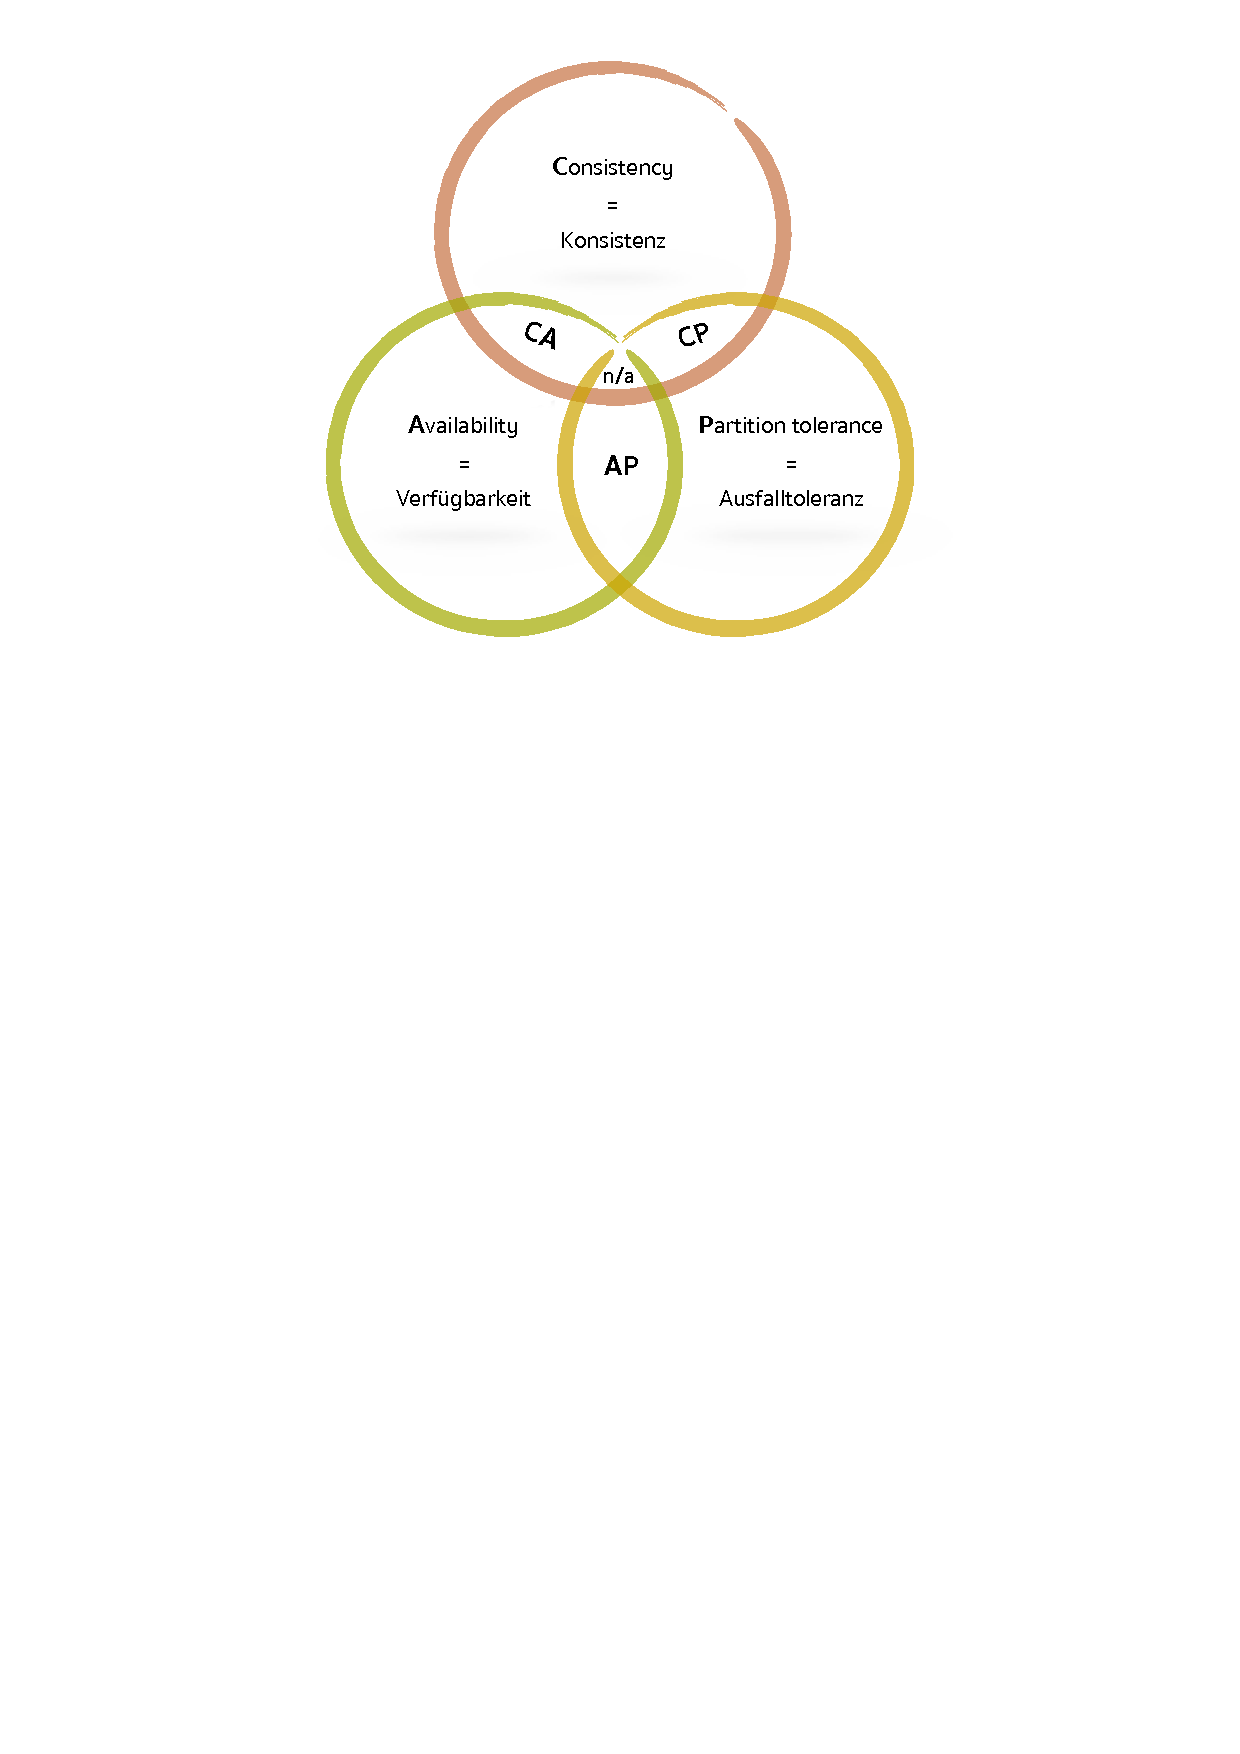
\includegraphics[trim = 0mm 189mm 0mm 9mm, clip, width=1.0\textwidth]{resources/myPictureForCAP}
\caption[\textbf{CAP}-Theorem]{Anforderungen an verteilte Systeme gemäß dem \textbf{CAP}-Theorem}
\label{img:cap}
\end{figure}

Das Akronym \textbf{CAP} steht für die englischsprachigen Begriffe  \Cap, \cAp\ und \caP. Diese sind mögliche Anforderungen an eine verteilte Anwendung.
\begin{itemize}
\item \Cap: Diese Anforderung ist erfüllt, wenn nach Abschluss einer atomaren\footnote{Eine atomare Transaktion bedeutet, dass sie entweder ganz oder gar nicht ausgeführt wird. Falls eine atomare Transaktion abgebrochen wird, werden alle im Laufe der Transaktion bereits durchgeführte Änderungen rückgängig gemacht.} Transaktion (oder Interaktion mit dem System) nicht nur die manipulierenden Datensätze, sondern auch alle replizierenden Knoten in einem großen Cluster über die gleichen Daten verfügen. Wenn ein Wert auf einem Knoten geändert wird und die Interaktion mit dem System abgeschlossen wird, muss der aktualisierte Wert von anderen Knoten zurückgeliefert werden können. Dies hat zur Folge, dass ein System erst dann die Interaktion abschließen darf, wenn sichergestellt ist, dass die Änderungen auf alle Datenkopien angewendet wurden. Für die verteilten Systeme, die Daten replizieren, resultiert es in langen Antwortzeiten für die Schreiboperationen.

\item \cAp: Die \textit{Hochverfügbarkeit} ist eine weitere Anforderung, die besagt, dass immer alle gesendeten Anfragen durch User an das System mit einer akzeptablen Reaktionszeit beantwortet werden müssen.

\item \caP: Die \textit{Partitions- oder Ausfalltoleranz} bedeutet, dass der Ausfall eines Knoten bzw. eines Servers aus einem Cluster das verteilte System nicht beeinträchtigt und es weiterhin fehlerfrei funktioniert. Falls einzelne Knoten in so einem System ausfallen, wird deren Ausfall mit den verbleibenden Knoten aus dem Cluster kompensiert, um die Funktionsfähigkeit des Gesamtsystems aufrecht zu halten.

\end{itemize}

Die graphische Darstellung für das Brewer's \textbf{CAP}-Theorem ist aus der Abbildung \ref{img:cap} zu entnehmen. Wie die Abbildung \ref{img:cap} erkennen lässt, können in einem verteilten System gleichzeitig und vollständig nur zwei von drei Anforderungen  \Cap, \cAp, \caP\ erfüllt werden. Konkret aus der Praxis bedeutet das, dass es für eine hohe Verfügbarkeit und Partitions- oder Ausfalltoleranz notwendig ist, die Anforderungen an die Konsistenz zu lockern \cite[S. 31]{Edlich.2011}.

Die Anforderungen in Paaren klassifizieren gemäß dem \textbf{CAP}-Theorem bestimmte Datenbanktechnologien. Für jede Webanwendung muss daher individuell entschieden werden, ob sie als ein \textbf{CA-}, \textbf{CP-} oder \textbf{AP-}System zu realisieren ist.
\begin{itemize}
\item \textbf{CA} (\textbf{C}onsistency und \textbf{A}vailability): Die klassischen relationalen Datenbankmanagementsysteme (RDBMS) wie Oracle, DB2 etc. fallen in \textbf{CA}-Kategorie, die vor allem auf  \Cap\ und \cAp\ aller Knoten in einem Cluster hinzielen. Hierbei werden die Daten nach dem \textbf{ACID}-Prinzip verwaltet. Die relationalen Datenbanken sind für Ein-Server-Hardware konzipiert und vertikal skalierbar. Das bedeutet, dass solche Systeme mit hochverfügbaren Servern betrieben werden und \caP\  nicht unbedingt in Frage kommt.

%\begin{itemize}
%\item keine Partitionstoleranz
%\item (Relationale) Datenbank ermöglicht verteilte Transaktionen zur Konsistenzwahrung
%\item Voraussetzung: funktionierendes Netzwerk (kein Nachrichtenverlust)
%\item URL: \url{http://dbs.uni-leipzig.de/file/NoSQL_SS14_01_Intro.pdf}
%\end{itemize}

\item \textbf{CP} (\textbf{C}onsistency und \textbf{P}artition tolerance): Ein gutes Beispiel für die Webanwendungen, die zu der \textbf{CP-}Kategorie zuzuordnen sind, sind Banking-Anwendungen. Für solche Anwendungen ist es wichtig, dass die Transaktionen zuverlässig durchgeführt werden und der mögliche Ausfall eines Knotens verschmerzt werden kann. 
%
%\begin{itemize}
%\item keine Verfügbarkeit
%\item im Falle von Netzwerkpartitionierung werden Transaktionen blockiert
%\item Vermeidung möglicher Konflikte bei Merge, dadurch Sicherstellung der Konsistenz
%\item URL: \url{http://dbs.uni-leipzig.de/file/NoSQL_SS14_01_Intro.pdf}
%\end{itemize}

\item \textbf{AP} (\textbf{A}vailability und \textbf{P}artition tolerance): Für die Anwendungen, die in die \textbf{AP-}Kategorie fallen, rückt die Anforderung \Cap\ in den Hintergrund. Beispiele für solche Anwendungen sind die Social-Media-Sites wie Twitter oder Facebook, da die Hauptidee der Anwendung nicht verfällt, wenn zum gleichen Zeitpunkt die replizierten Knoten nicht die gleiche Datenstruktur aufweisen. 
\end{itemize}
%
%\begin{itemize}
%\item keine Konsistenz
%\item Writes stets möglich auch wenn keine Kommunikation mit anderen Knoten möglich
%(z.B. Synchronisation)
%\item Notwendigkeit der Auflösung inkonsistenter Daten, d.h. verschiedene Versionen des
%selben Datums an verschiedenen Knoten
%\item URL: \url{http://dbs.uni-leipzig.de/file/NoSQL_SS14_01_Intro.pdf}
%\end{itemize}

\subsubsection{Das BASE-Prinzip}\label{base}
%\subsubsection{\colorbox{green}{Das BASE-Prinzip}}\label{base}

\textbf{BASE} steht für \BAse, \baSe, \basE\ und beschreibt eine Alternative zu den strengen \textbf{ACID}-Kriterien.
Bei den Systemen, die nach dem \textbf{BASE}-Prinzip gestaltet sind, wird bewusst in Kauf genommen, dass die Daten nach Schreiboperationen eine absehbare Zeit inkonsistent sein können.

Bei solchen Systemen ist viel mehr die permanente Verfügbarkeit des Systems für die Clients wichtig, als die Möglichkeit, die gleichen Daten zu dem sofortigen Zeitpunkt zu sehen. Nach Ablauf einer gewissen Zeit muss das System den inkonsistenten Zustand der Daten wieder in einen konsistenten Zustand bringen, so dass alle Clients die gleichen Daten sehen können\footnote{Das BASE-Prinzip, \url{https://blog.codecentric.de/2011/08/grundlagen-cloud-computing-cap-theorem/}, zugegriffen am 05. Februar 2017}.

\begin{itemize}
\item \BAse\ bedeutet, dass ein System immer verfügbar ist und eine Antwort immer zurückkommt. Die gelieferten Daten müssen nicht konsistent sein. Es können inzwischen Updates geben, die zwar den Datenstand geändert haben, allerdings mit dem Knoten, der geantwortet hat, noch nicht synchronisiert wurden.

\item \baSe\ kennzeichnet, dass der Datenzustand nicht unbedingt alle Updates abbildet, die bisher eingegangen sind. Es können Updates geben, die noch nicht überall angewendet wurden.

\item \basE\ besagt, dass sich das System in einem konsistenten Zustand befindet, wenn alle eingegangenen Update-Operationen auf den Daten überall angewendet wurden und keine neuen Daten zwischenzeitlich eingegangen sind.\footnote{ACID vs. BASE, \url{http://www.dataversity.net/acid-vs-base-the-shifting-ph-of-database-transaction-processing/}, zugegriffen am 14. Februar 2017}
\end{itemize}

\subsection{Wartbarkeit}\label{maintenance}
%\subsection{\colorbox{green}{Wartbarkeit}}\label{maintenance}

Um die Wartungs- und Erweiterungsfähigkeiten von der Software zu gewährleisten, sollen die grundlegenden Designprinzipien eingehalten werden.

\subsubsection{Die SOLID-Prinzipien}\label{solid}
%\subsubsection{\colorbox{green}{Die SOLID-Prinzipien}}\label{solid}

Das von Martin Fowler geprägtes Akronym \textbf{SOLID}\footnote{SOLID, \url{https://web.archive.org/web/20150906155800/http://www.objectmentor.com/resources/articles/Principles_and_Patterns.pdf}, zugegriffen am 03.02.2017} steht für fünf Prinzipien des objektorientierten Designs. Bei korrekter Anwendung dieser Prinzipien erfolgt eine höhere Wartbarkeit am Softwareprodukt. Die Software, die mit der Einhaltung von \textbf{SOLID} Regeln entwickelt wird, besteht aus vielen kleinen Modulen. Jedes Modul übernimmt bei der Entwicklung eine klare Funktion und die Interaktion zwischen diesen Modulen erfolgt über die explizit definierten Schnittstellen.

Im Einzelnen beschreibt \textbf{SOLID} folgende Regeln:

\begin{itemize}

\item \textit{\textbf{S}ingle responsibility principle} - Eine Klasse (oder Modul) soll nur eine bestimmte Funktion abdecken und eine Funktion soll von einer Klasse implementiert werden. Martin Fowler nach, kann es für die Änderung einer Klasse nur einen Grund geben. Im Kontext der Prototypanwendung könnte der Backend-Teil beispielsweise zwei Funktionen haben, die Bearbeitung von Frontend-Anfragen und Verwaltung der Daten in der Datenbank. Demnach wäre das Design schlecht, wenn eine Klasse beide diese Funktionalitäten implementieren würde. In diesem Fall gäbe es mehrere Gründe für die Änderung dieser Klasse - z. B. eine Änderung in Kommunikation mit Frontend oder in der Datenhaltung.

\item \textit{\textbf{O}pen/closed principle} - Die Klassen/Module sollen für die Erweiterung offen sein, die bestehenden Klassen sollen jedoch nicht geändert werden. Die Idee, die dahinter steht, kann folgendermaßen zusammengefasst werden. Sofern die neuen Funktionalitäten eingeführt werden, darf der bestehende Code nur minimal geändert werden. Beispielsweise wurden die Daten der Foto-Verwaltungs-Anwendung bisher in der relationalen Datenbank abgelegt und zusätzlich soll die Datenhaltung in der NoSQL-Datenbank implementiert werden. Die NoSQL-Datenhaltung soll in eigenem Modul implementiert werden, dadurch darf die Codebasis für die Interaktion mit relationaler Datenbank nicht geändert werden. 

\item \textit{\textbf{L}iskov substitution principle} - Die Subklassen dürfen das Verhalten der Elternklassen nicht ändern. Der Code, der auf bestehenden Funktionen der Elternklassen aufgebaut ist, muss auch mit Subklassen fehlerfrei funktionieren.

Wenn z. B. die Foto-Verwaltungs-Anwendung erweitert wird und z. B. die Videos verwaltet werden sollen, wäre es falsch, die Klasse \textit{`Video`} aus der Klasse \textit{`Foto`} abzuleiten, weil Videos andere Eigenschaften als Bilder haben.

\item \textit{\textbf{I}nterface-segregation principle} - Die Interfaces sollen so klein wie möglich sein und nur einzelne Funktionen abdecken.

\item \textit{\textbf{D}ependency inversion principle} - Die Abhängigkeiten zwischen Modulen sollen über Abstraktionen \textit{(Interfaces)} gekoppelt werden. Ein Modul soll eine direkte Abhängigkeit zu den anderen Modulen vermeiden, die Abhängigkeiten werden zu den Interfaces definiert. Demzufolge können die Module die Interfaces implementieren und ohne großen Aufwand ausgetauscht werden. 

Für die Module sind nur die Interfaces sichtbar, die zu implementieren sind. Es können keine Annahmen getroffen werden, welche Teile der Anwendung diese Module verwenden werden. Sie sollen überall einsetzbar sein, wo sie ihre Funktion, die in dem Interface definiert ist, erfüllen können. Als Beispiel wird erneut Backend der Foto-Verwaltungs-Anwendung genommen und die Interaktion zwischen dem \textit{Service}-Modul betrachtet, das mit Frontend interagiert und dem Modul, das Daten in der relationalen Datenbank verwaltet. Anstatt eine Referenz zu diesem spezifischen Datenbankmodul zu deklarieren, wird eine Referenz zu einem Interface deklariert, das die Datenhaltungskomponente beschreibt. Aus der Sicht des \textit{Service}-Moduls gibt es eine Menge von notwendigen Operationen zum Speichern oder zum Abrufen der Daten. Diese Operationen sind unabhängig von der Art der Daten ähnlich aufgebaut und deswegen werden sie in einem \textit{Interface} zusammengefasst. Das \textit{Service}-Modul deklariert eine Abhängigkeit zu diesem \textit{Interface}. Dieses \textit{Interface} kann von verschiedenen Datehaltungskomponenten implementiert werden.

\end{itemize}

\subsubsection{Dependency Injection (DI)}\label{di}
%\subsubsection{\colorbox{green}{Dependency Injection (DI)}}\label{di}

\textit{Dependency Injection} ist der nächste Schritt nach \textit{Dependency Inversion}. Das \textit{Dependency Injection Pattern} basiert auf dem \textit{Inversion of Control Konzept}. Das bedeutet, dass sich die verwendeten Klassen nicht mehr selbst um Ablauf und Abhängigkeiten kümmern, sondern diese werden an eine externe Komponente ausgelagert. Die Klasse gibt vermeintlich die Kontrolle ab und lässt sich von außen steuern. Konkret bedeutet es, dass die Klassen nur die Abhängigkeiten zu den Interfaces deklarieren müssen und die konkrete Implementierung zur Laufzeit eingefügt (injected) wird. 

Die genauere Zusammensetzung einer Anwendung wird deklarativ definiert, sodass verschiedene Konfigurationen existieren können.

Die Einhaltung des \textit{Dependency Inversion} Prinzips zusammen mit der Anwendung des \di\ Patterns ermöglicht den Entwicklern, den Arbeitsaufwand für die Entwicklung großer Anwendungen stark zu reduzieren.
Es wird eine \textbf{lose Kopplung} der Anwendungskomponenten erreicht, die dem Entwickler die Konzentration auf die Entwicklung einzelner Komponenten unabhängig voneinander ermöglicht. Die Unabhängigkeit der Programmteile erleichtert dem Entwickler nicht nur die Anwendungskomponenten unabhängig voneinander zu entwicklen, sondern auch diese leichter zu testen. 

\subsubsection{Dependency Injection und Mock-Objekte}
%\subsubsection{\colorbox{green}{Dependency Injection und Mock-Objekte}}\label{di}

Enge Kopplung von Abhängigkeiten erschwert nicht nur die Erweiterung oder Änderung von Codebasis, sondern auch die Testbarkeit. Beispielsweise sollten die Komponenten unabhängig von den anderen Komponenten mit \textit{UnitTests} getestet werden. Dafür werden die Abhängigkeiten zu anderen Komponenten simuliert. Falls die zu testende Methode die Daten aus der Datenbank für die Berechnung benötigt, kann die Datenbankverbindung simuliert und die Testdaten zurückgegeben werden. Solche Klassen, die die Abhängigkeiten simulieren, nennt man \textbf{Mock-Klassen}.

Die lose Kopplung des \textit{DI} Patterns ermöglicht die Verwendung von Mock-Objekten. Die entsprechenden Abhängigkeiten werden zur Laufzeit von Tests von dem entsprechenden Framework injiziert, sodass seitens des Entwicklers keine weiteren Schritte notwendig sind.

\subsubsection{MVC-Pattern}\label{mvc}
%\subsubsection{\colorbox{green}{MVC-Pattern}}\label{mvc}

\textbf{MVC}\footnote{Objektorientierte Programmierung, \url{http://openbook.rheinwerk-verlag.de/oop/oop_kapitel_08_002.htm}, zugegriffen am 20. Januar 2017} ist ein Prinzip der modernen Programmierung und ist nach wie vor das wichtigste und verbreitetste Muster für die Architektur von GUI-Anwendungen. Solche Architektur kommt fast bei allen GUI-Frameworks zum Einsatz.

Das Ziel des \textbf{MVC}-Musters ist, die Geschäftslogik einer Anwendung von der Benutzerschnittstelle abzutrennen, so dass ein Entwickler einen Bereich bequem verändern kann und der Rest der Anwendung dadurch nicht beeinflusst wird. Es soll einen flexiblen Programmierentwurf geben, der eine spätere Änderung oder Erweiterung erleichtert und eine Wiederverwendbarkeit und Austauschbarkeit einzelner Komponenten ermöglicht.

\paragraph{Workflow}
%\paragraph{\colorbox{green}{Workflow}}

Der Workflow-Prozess \textbf{(Abb. \ref{img:mvc})} stellt eine vollständige Beschreibung aller Aktivitäten, der den Einsatz des \textbf{MVC}-Patterns voraussetzt. Die Abbildung \ref{img:mvc} stellt einen groben Workflow des \textbf{MVC}-Patterns anhand einer Beispielinteraktion und ihres Ergebnisses dar.
\begin{figure}[H]
\centering
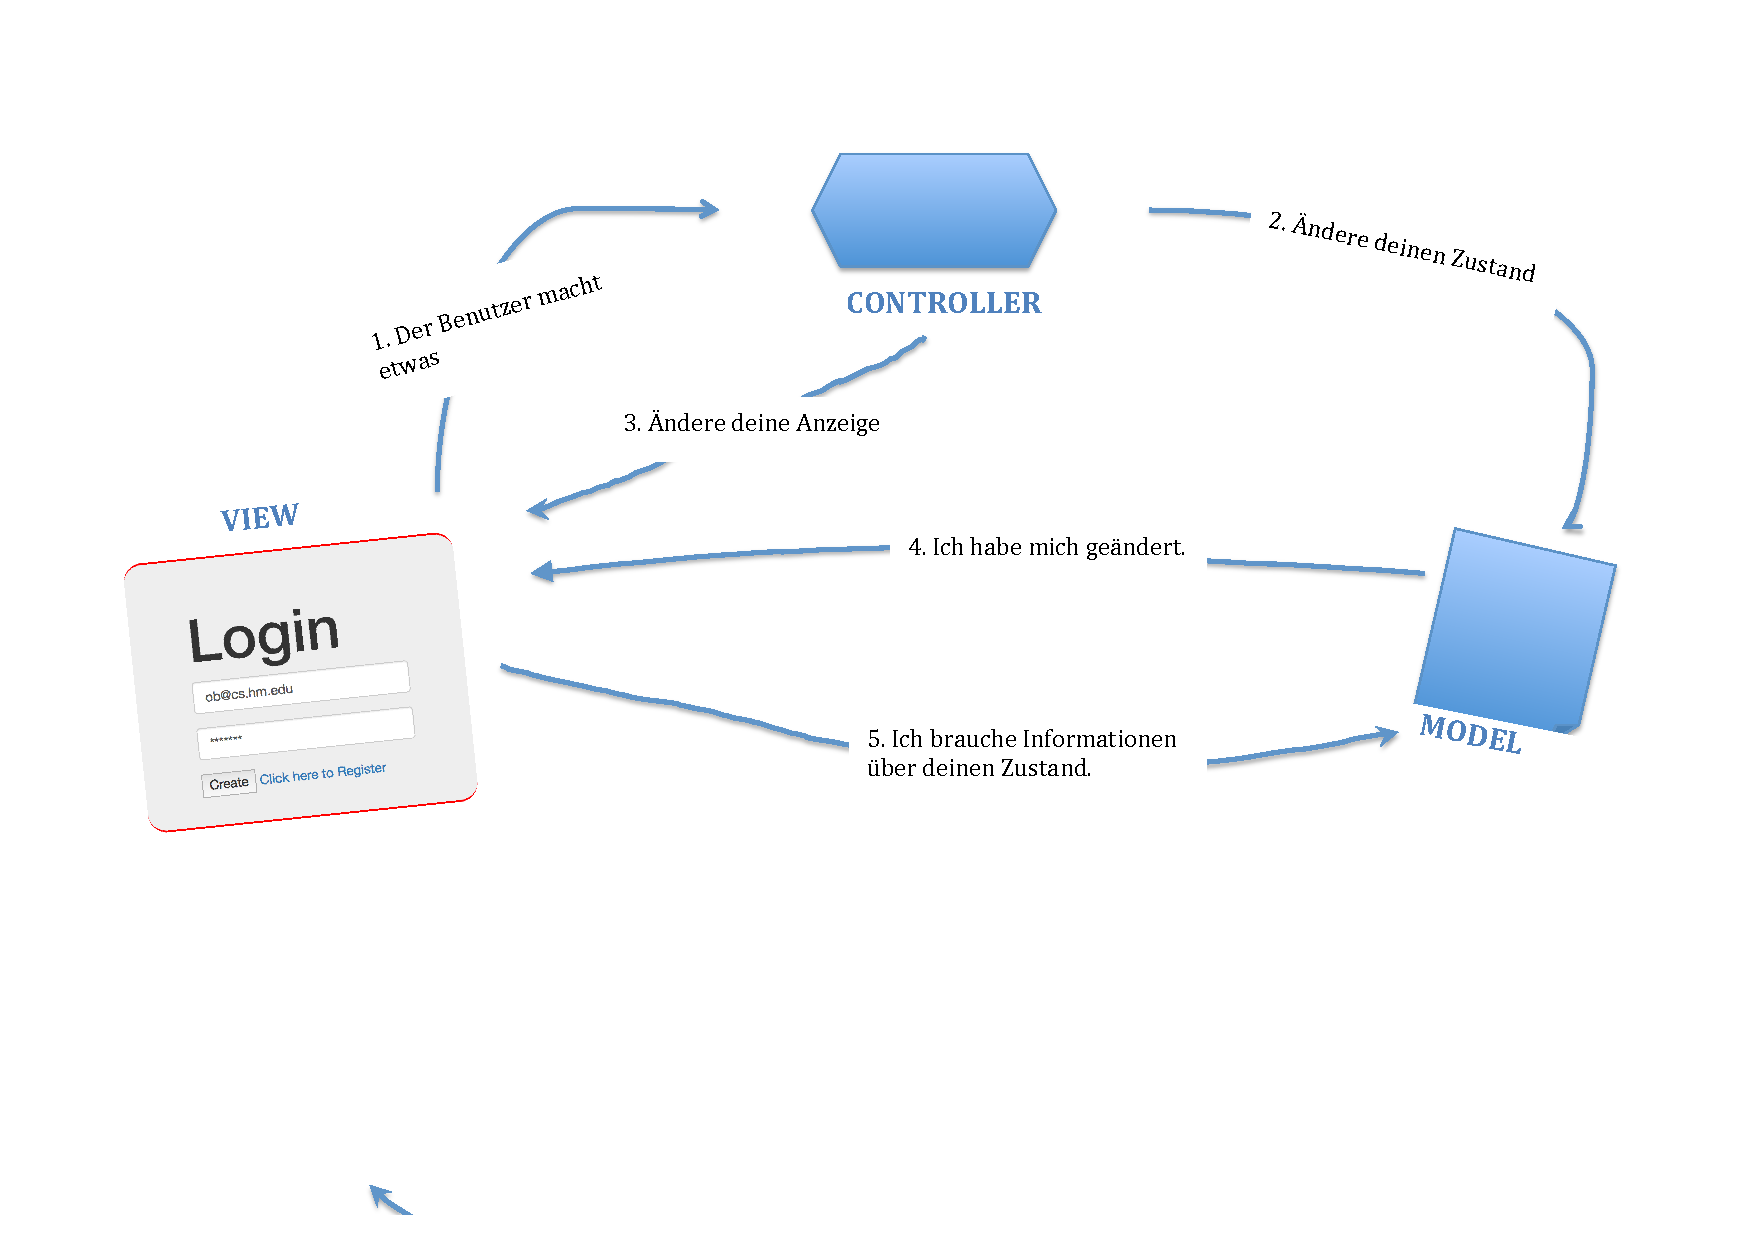
\includegraphics[trim = 0mm 60mm 0mm 20mm, clip, width=1.0\textwidth]{resources/mvc}
\caption[Workflow zum MVC-Konzept]{Workflow zum MVC-Konzept}
\label{img:mvc}
\end{figure}

\textbf{Beschreibung des Workflow-Prozesses:}
\begin{enumerate}
\item \textbf{Der Benutzer interagiert mit der View}

Der Benutzer führt eine Aktion an der View aus. Dadurch teilt die View dem Controller mit, was zu tun ist. Erst dann ist die Aufgabe des Controllers, entsprechende Steuerungsmaßnahmen zu ergreifen.

\item  \textbf{Der Controller fordert das Model auf, seinen Zustand zu ändern}

Nach der Ausführung einer Aktion an der View durch den Benutzer, nimmt der Controller diese Aktion an und interpretiert sie. Bei der Interpretation stellt der Controller fest, was gemacht werden muss und wie das Model aufgrund dieser Aktion beeinflusst werden kann.

\item  \textbf{Der Controller kann auch die View auffordern, ihren Zustand zu ändern}

Der Controller kann bei der Ausführung einer Aktion auch die View auffordern, sich zu ändern. Zum Beispiel, beim Klick auf einen Button durch den Benutzer kann die gerade eingeblendete View ausgeblendet und eine andere View eingeblendet werden.

\item  \textbf{Das Model informiert die View über seine Zustandsänderung}

Dem Model selbst sind Views und Controller nicht bekannt bzw. diese sind an dem Model nicht festprogrammiert. Aber das Model kann diejenigen, die sich beim Model registriert haben, über seine Zustandsänderungen informieren.

\item  \textbf{Die View erfragt den Zustand des Models}

Das Model stellt weitere Methoden zur Verfügung, über die der aktuelle Zustand des Models erfragt werden kann. Jede View kann sich somit durch den Aufruf dieser Methoden über den Zustand des Models informieren.

\end{enumerate}
Um die Benachrichtigung über Modelsänderungen an Views oder auch an Controller zu realisieren, nutzt MVC das sogenannte Beobachter Muster.

\paragraph{Beobachter Muster}\label{observer}
%\paragraph{\colorbox{green}{Beobachter Muster}}\label{observer}

Beobachter Muster (engl. Observer-Pattern) ist eines der am meisten genutzten und bekanntesten Patterns. In diesem Muster teilt die Komponente Model allen Interessenten proaktiv mit, dass ihr Zustand geändert wurde.

Würde man ohne das \textbf{Observer}-Pattern eine solche `Beobachtung` implementieren, so müssten die Interessenten die Komponente Model regelmäßig abfragen, ob ihr Zustand geändert wurde.

Beim \textbf{Observer}-Pattern gibt es eine Komponente (Observable), deren Zustand sich ändern kann und andere Komponenten (Observers), die über Zustandsänderung informiert werden sollten. Das \textbf{Observer}-Pattern sieht vor, dass sich die Observers beim Observable registrieren und bei einer Zustandsänderung alle registrierte Objekte informiert.

\begin{figure}[H]
\centering
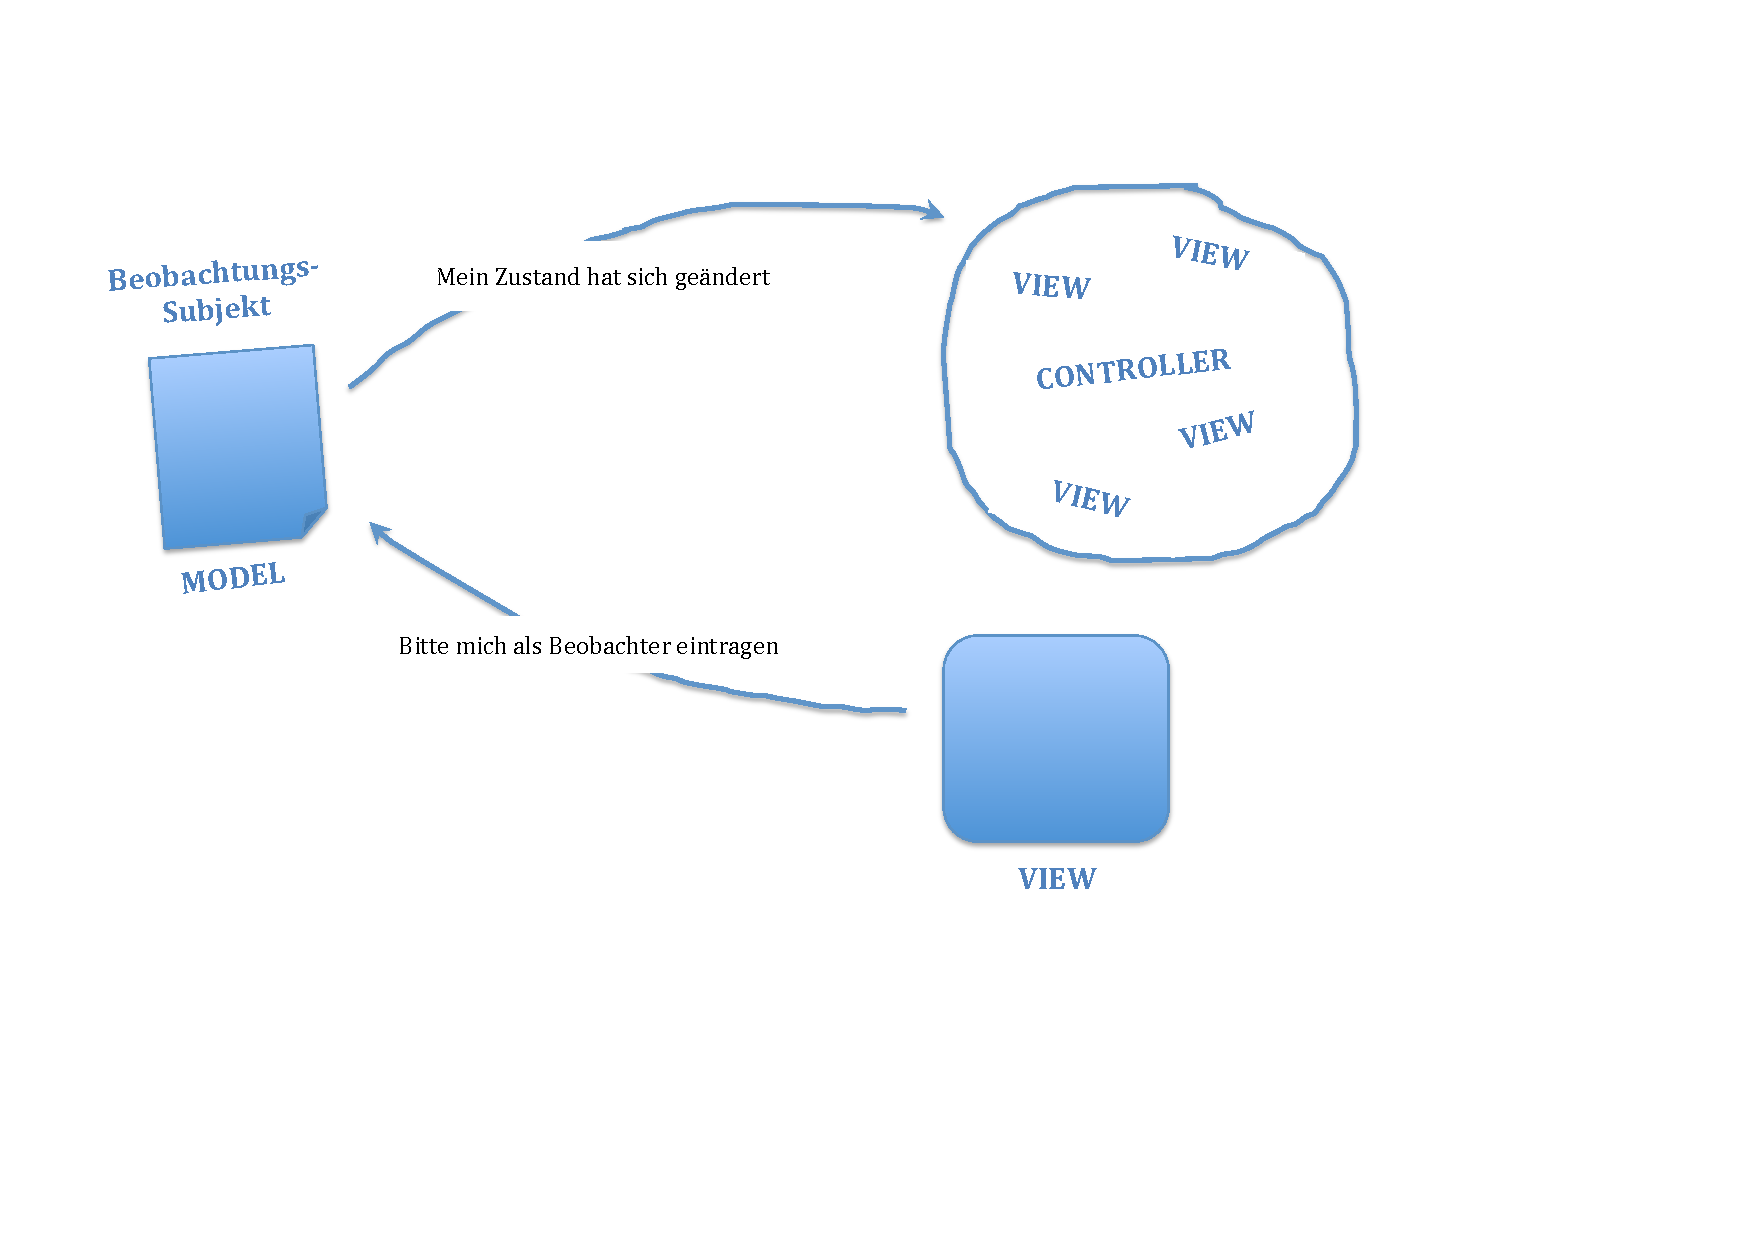
\includegraphics[trim = 0mm 0mm 0mm 0mm, clip, width=0.8\textwidth]{resources/observer}
\caption[Observer Pattern]{Observer Pattern}
\label{img:observer}
\end{figure}

\textbf{Beschreibung des \textbf{Observer}-Pattern Prinzips:}

Die Abbildung \ref{img:observer} zeigt, wie \textbf{Observer}-Pattern im \textbf{MVC} verwendet wird. Wenn eine View bei einer Zustandsänderung des Models informiert werden möchte, registriert sie sich beim Model. Die View wird somit in die Liste hinzugefügt, in der sich bereits andere Observers befinden können. Im Fall einer Zustandsänderung läuft das Model die Liste durch und informiert somit alle, die sich als Beobachter eingetragen haben.

%\section{Relevante Technologien}
\section{\colorbox{yellow}{Relevante Technologien}}

Dieser Abschnitt widmet sich den aktuellen Technologien, die für den Prototyp relevant sind.

\subsection{NoSQL-Datenbanken}
%\subsection{\colorbox{yellow}{NoSQL-Datenbanken}}

Im Vergleich zu den relationalen Datenbanken, die sich als eine strukturierte Sammlung von Tabellen (den Relationen) vorstellen, in welchen Datensätze abgespeichert sind, eignen sich \textit{NoSQL}-Datenbanken zur unstrukturierter Daten, die einen nicht-relationalen Ansatz verfolgen. 

Der Begriff NoSQL steht nicht für 'kein SQL', sondern für 'nicht nur SQL' (Not only SQL). Das Ziel von NoSQL ist, relationale Datenbanken sinnvoll zu ergänzen, wo sie Defizite aufzeigen. Entstanden ist dieses Konzept in erster Linie als Antwort zur Unflexibilität, sowie zur relativ schwierigen Skalierbarkeit von klassischen Datenbanksystemen, bei denen die Daten nach einem stark strukturierten Modell gespeichert werden müssen.\footnote{MySQL vs. MongoDB: \url{http://www.computerwoche.de/a/datenbanksysteme-fuer-web-anwendungen-im-vergleich,2496589}, zugegriffen am 3. Januar 2016} Dokumentdatenbanken gruppieren die Daten in einem strukturierten Dokument, typischerweise in einer \textit{JSON}\footnote{JSON, \url{http://www.json.org}}-Datenstruktur. \mongo\ ist eine von vielen NoSQL-Datenbanken, die auch diesen Ansatz verfolgt und bietet darauf aufbauend eine reichhaltige Abfragesprache und \textit{Indexe} auf einzelne Datenfelder. Die Möglichkeiten der \textit{Replikation} und des \textit{Shardings} zur stufenlosen und unkomplizierten Skalierung der Daten und Zugriffe macht \mongo\ auch für stark frequentierte Websites äußerst interessant.(\cite{Hollosi.2012}, Kapitel 14, Seite 435)

Beispiele für NoSQL-Datenbanken:
\begin{multicols}{2}
\begin{itemize}
\item CouchDB
\item MongoDB
\item Redis
\item Google BigTable
\item Amazon Dynamo
\item Apache Cassandra
\item Hbase (ApacheHadoop)
\item Twitter Gizzard
\item weitere…
\end{itemize}
\end{multicols}

Jede NoSQL-Datenbank verfolgt seine eigenen Ziele und ist kategorisiert. Die möglichen Kategorien werden demnächst näher erläutert.

\begin{itemize}
\item Eine Key-Value-Datenbank \textit{(Key-Value Store)} ist eine Datenbank, in der die Daten in Form von Schlüssel-Werte-Paaren abgespeichert werden. Der Schlüssel verweist dabei auf einen eindeutigen (meist in Binär- oder Zeichenketten-Format vorliegenden) Wert\footnote{NoSQL: Key-Value-Datenbank Redis im Überblick: \url{https://www.heise.de/developer/artikel/NoSQL-Key-Value-Datenbank-Redis-im-Ueberblick-1233843.html}, zugegriffen am 17. Januar 2017}. Value kann oft beliebiger Datentyp wie Arrays, Dokumente, Objekte, Bytes etc. sein.

\item In einer spaltenorientierten Datenbank \textit{(Column Store)}, wie der Name vermuten lässt, werden die Datensätze spalten- statt zeilenweise abgespeichert. Durch die spaltenorientierte Abspeicherung der Daten wird der Lesezugriff stark beschleunigt, da keine unnötigen Informationen mehr gelesen werden, stattdessen nur diejenigen, die wirklich benötigt wurden. Dadurch wird der Schreibprozess aber erschwert, falls die schreibenden Daten aus mehreren Spalten bestehen werden, auf die entsprechend zugegriffen werden muss. Der Schreibprozess wird sich in diesem Fall etwas verlangsamen.

\item Eine Graphen-Datenbank \textit{(Graph database)} ist die weitere Kategorie aus der NoSQL Gruppe, in der die Daten anhand eines Graphen dargestellt und abgespeichert werden.

Die Graphen bestehen grundsätzlich aus Knoten \textit{(Node)} und Kanten \textit{(Edge)}. Dabei stellen die Kanten die Verbindungen zwischen den einzelnen Knoten dar.

\item Eine Datenbank, in der die Daten in Form von Dokumenten abgespeichert werden, ist als eine dokumentenorientierte Datenbank \textit{(Document Store)} zu definieren. In diesem Zusammenhang ist ein Dokument als eine Zusammenstellung bestimmter Daten zu verstehen, das mit einem eindeutigen Identifikator angesprochen werden kann. Da die Daten in der dokumentenorientierten Datenbank nicht in Form von Tabellen, sondern in Form von Dokumenten abgespeichert werden, ergibt sich daraus keinen Strukturzwang.

Möchte man ein bestimmtes Dokument erweitern, so kann man es einfach tun, da eine dokumentenorientierte Datenbank strukturfrei ist. Weitere Datenformate sind beispielsweise YAML\footnote{YAML: \url{http://www.yaml.org/start.html}} (angelehnt an XML) oder XML\footnote{XML: \url{https://www.xml.com/}} selbst. 
\end{itemize}

%Bei dem Auswahl einer Datenbank für Foto-Verwaltungs-Service fiel die Entscheidung auf eine der NoSQL-Datenbank \mongo. Laut DB-Ranking\footnote{DB-Ranking: \url{http://db-engines.com/de/ranking}, zugegriffen am 13. März 2017} ist die \mongo\ einer der populärsten Datenbanken aus der NoSQL-Gruppe und passt ideal für Webprojekte mit \textit{Big Data}.

\subsubsection{MongoDB}\label{mongo}
%\subsubsection{\colorbox{green}{MongoDB}}\label{mongo}

\mongo\ ist eine  schemalose, dokumentenorientierte Open-Source-Datenbank. Der Name stammt von dem englischen Begriff \textit{hu}MONGO\textit{us}, ins Deutsche als \textit{gigantisch} oder \textit{riesig} übersetzen lässt.


%\rowcolors{1}{white}{lightgray}
%\newcommand*{\head}[1]{\textbf{#1}}%
%
%\rowcolors{2}{gray!25}{white}
%\begin{table}[h]
%\centering
%\begin{tabular}{cc}
%\toprule 
%    \rowcolor{gray!50}
%	Relational & \mongo\ \\
%	\midrule
%	Database &  Database\\
%	Table & Collection\\
%	Row &  Document\\
%	Column &  Field\\
%	Index & Index\\
%	Join &  Embedding and Linking\\
%	Primary key & \textit{\_id}-Field (default)\\
%	\bottomrule
%\end{tabular}
%\caption[Konzepte im Vergleich]{Konzepte im Vergleich}
%\label{table:concepts}
%\end{table}

\mongo\ präsentiert sich als eine quelloffene, dokumentenorientierte NoSQL-Datenbank mit den folgenden Konzepten wie \textit{Ausfallsicherheit} und \textit{horizontale Skalierung} (\textbf{Kap. \ref{cap}}).
%Die Unterschiede zu den Konzepten der relationalen und nicht-relationalen Datenbanken, konkret von \mongo\ stellt die Tabelle \ref{table:concepts} dar.

\paragraph{Datensätze in Form von Dokumenten}
%\subsection{Datensätze in Form von Dokumenten}
%Die Datensätze werden in  der NoSQL-Datenbank \mongo\ in Dokumente gespeichert. \mongo\ verwendet für die Dokumentenspeicherung und den Datenaustausch das sogenannte \textit{BSON}\footnote{BSON: \url{http://www.bjson.org}}-Format, das eine binäre Darstellung von \textit{JSON}-ähnlichen Dokumenten bietet. Nachfolgend sind alle für \textit{BSON} definierten Datentypen aufgelistet:
%\begin{multicols}{3}
%\begin{itemize}
%\item Double
%\item String
%\item Object
%\item Array
%\item Binary Data
%\item Undefined
%\item Object Id
%\item Boolean
%\item Date
%\item Null
%\item Regular Expression
%\item JavaScript
%\item Symbol
%\item JavaScript(with scope)
%\item 32-Bit Integer
%\item Timestamp
%\item 64-Bit Integer
%\item Min Key
%\item Max Key
%\end{itemize}
%\end{multicols}
%Der Grund für die große Anzahl an Datentypen ist ein wesentliches Ziel der Entwickler von \textbf{BSON}: \textit{Effizienz.}

%speichert Daten in Form von Dokumenten im \textbf{BJSON}\footnote{BSON: \url{http://www.bjson.org}}-Format.
Die Dokumente selbst werden von \mongo\ in sogenannten Kollektionen \textit{(Collections)} gespeichert, die grob mit den Tabellen einer relationalen Datenbank vergleichbar sind. Ein Zugriff auf Daten mehrerer Kollektionen \textit{(Collections)}, wie es aus dem \textit{Joins}-Konzept relationaler Datenbank bekannt ist, ist nicht möglich. Die \textit{CRUD}-Operationen sind auf Ebene der \textit{Collection} durchzuführen. Jedes Dokument ist an keine vordefinierte Struktur gebunden und kann eine beliebige Anzahl an Feldern besitzen. Die Dokumente aus einer \textit{Collection} sind komplett unabhängig voneinander. 

Die Speicherung von Daten in Form von Dokumenten bietet den Vorteil, das sowohl strukturierte, als auch semi-strukturierte und polymorphe Daten gespeichert werden können. Dokumente, die jedoch das gleiche oder ein ähnliches Format haben, sollten zu einer Kollektion \textit{(Collection)} zusammengefasst werden\footnote{MongoDB: \url{http://www.moretechnology.de/mongodb-eine-dokumentenorientierte-datenbank/}, zugegriffen am 21. Januar 2017}.

%\paragraph{\colorbox{yellow}{Architektur}}
%%\subsection{Die Nexus Architektur}
%
%Zu den wichtigsten Eigenschaften, die für einen Einsatz von \mongo\ sprechen, gehören:
%\begin{itemize}
%\item Verfügbarkeit: Auch bei Ausfall einer Datenbankinstanz soll die Anwendung weiterhin verfügbar bleiben.
%\item Skalierbarkeit: Mit \textit{Sharding}, einem Verfahren zur horizontalen Skalierung, kann der effiziente Umgang mit großen Datenmengen erreicht werden.\footnote{MongoDB Eigenschaften: \url{https://entwickler.de/online/datenbanken/mongodb-erfolgreich-ein-dokumentenorientiertes-datenbanksystem-einfuehren-115079.html}, zugegriffen am 12. Dezember 2016}
%\end{itemize}

%Die Vorteile relationaler und NoSQL-Datenbanken sind aus der Abbildung \ref{img:architektur} zu entnehmen.
%\begin{figure}[H]
%\centering
%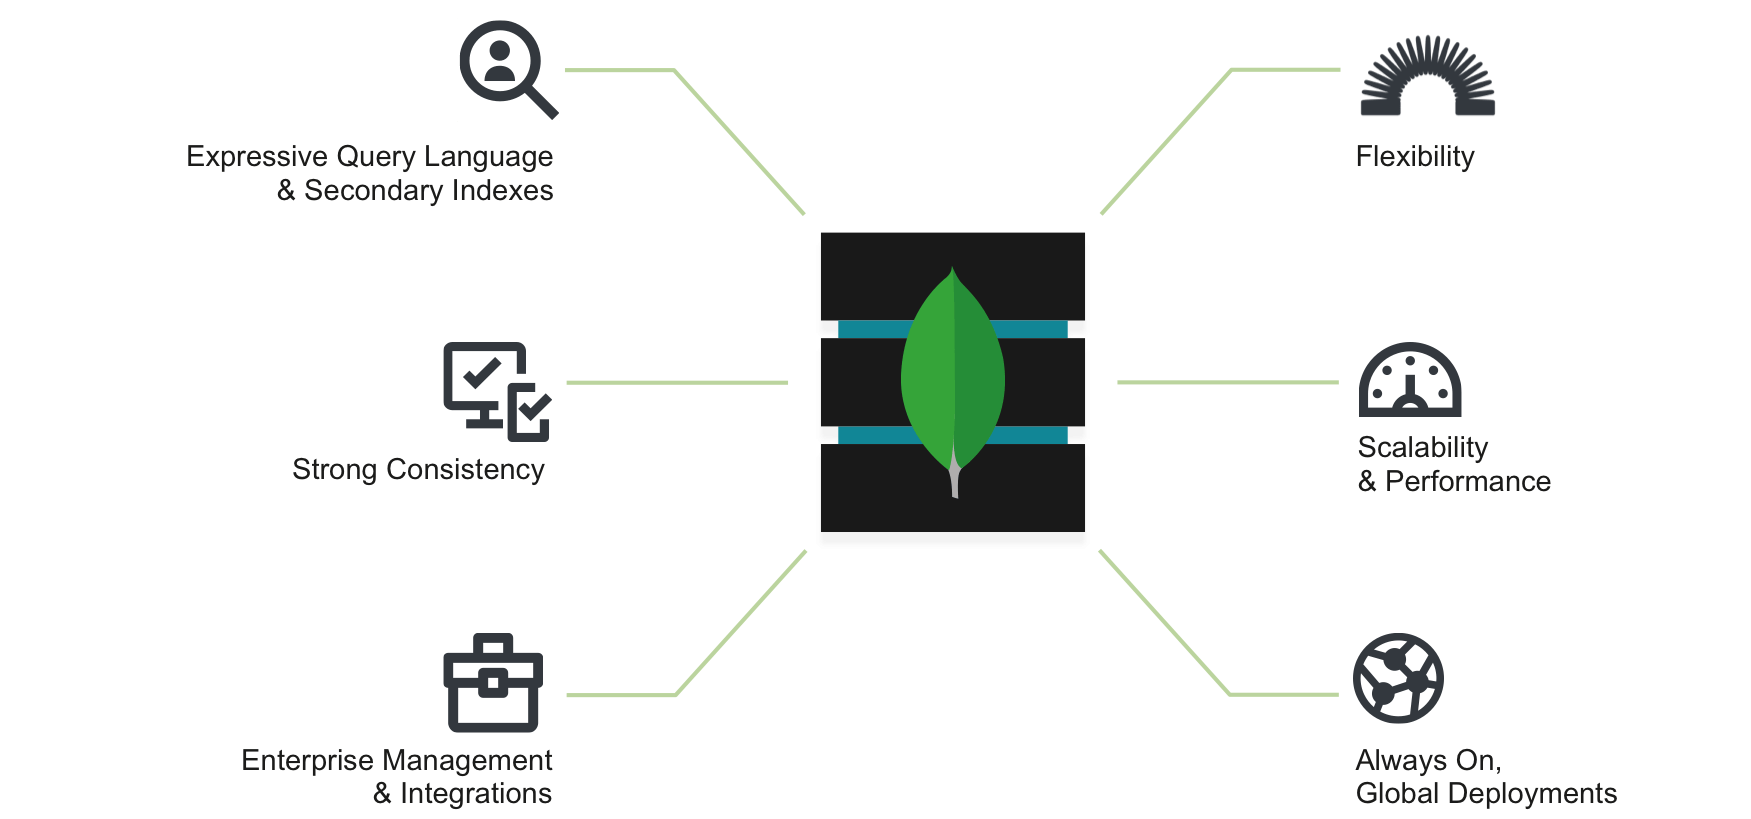
\includegraphics[width=1.0\textwidth]{resources/architecture}
%\caption[MongoDB Architektur]{MongoDB Architektur\protect\footnotemark}
%\label{img:architektur}
%\end{figure}
%\footnotetext{MongoDB Architektur: \url{https://www.mongodb.com/mongodb-architecture}, zugegriffen am 28. Januar 2016}


%\subsection{\colorbox{yellow}{Server/Client starten}}
%%\subsection{Server/Client starten}
%Zum Starten des Server-Prozesses muss im Terminal der folgende Befehl ausgeführt werden:
%\begin{listingsboxShell}[label={lst:serverStart}]{myshell}{Server-Prozess starten}
%vlfa:~ vlfa$ mongod
%\end{listingsboxShell}
%Mit dem Befehl
%\begin{listingsboxShell}[label={lst:mongoClient}]{myshell}{Client-Prozess starten}
%vlfa:~ vlfa$ mongo
%\end{listingsboxShell}
%wird ein Client-Prozess gestartet, falls die \textit{mongod-}Instanz aktiv ist.
%Nachdem das Client-Prozess gestartet ist, kann der Client an der Datenbank berühmte \textit{CRUD-}Operationen ausführen.
%
%Ohne irgendeine Konfiguration vornehmen zu müssen, verwendet \mongo-Server von Anfang an als Default den TCP-IP-Port 27017 für eingehende Verbindungen.
%
%\mongo\ unterstützt auch eine HTML-basierte Administrationsoberfläche. Falls sie benötigt wird, ist es möglich, im Terminal mit dem folgenden Befehl die HTML-basierte Administrationsoberfläche zu starten:
%\begin{listingsboxShell}[label={lst:html}]{myshell}{HTML-basierte Administrationsoberfläche starten}
%vlfa:~ vlfa$ mongod --httpinterface --rest
%\end{listingsboxShell}
%und dementsprechend sie im beliebigen Browser der folgenden URL aufzurufen:
%\begin{listingsboxShell}[label={lst:browser}]{myshell}{HTML-basierte Administrationsoberfläche aufrufen}
%http://localhost:28017/
%\end{listingsboxShell}
%Auf der Seite sind alle relevante Informationen zu Replikaktionsgruppen, Skalierung, verbundene Clients etc. zu finden.
%
%\paragraph{\colorbox{yellow}{CRUD = IFUR-Operationen}\label{ifur}}
\paragraph{CRUD = IFUR-Operationen}\label{ifur}
Die \textit{\textbf{CRUD}}-Operationen aus SQL heißen in \mongo\ \textit{\textbf{I}nsert}, \textit{\textbf{Fi}nd}, \textit{\textbf{U}pdate} und \textit{\textbf{R}emove}. Bei \mongo\ wird eine Datenbank bzw. eine Collection erst zur Laufzeit und beim ersten Einfügen des ersten Dokuments von \mongo\ selbst erzeugt. Die gesonderte Erstellung einer Datenbank oder einer Collection kann somit erspart werden.
\begin{itemize}
\item Für die Speicherung von neuen Dokumenten in der Datenbank bietet \mongo\ drei Funktionen an, welche als Parameter ein einzelnes oder eine Reihe von Dokumenten in einem Array annehmen. %Die \textit{Collection} muss vor dem Einfügen von neuen Dokumenten nicht explizit angelegt werden. Falls sie nicht existiert, wird sie zunächst erstellt und die übergebenen Dokumente eingefügt.
\begin{listingsboxShell}[label={lst:insert}]{myshell}{Dokument(e) speichern}
> db.<collection>.insert(<...>)
> db.<collection>.insertMany(<...>)
> db.<collection>.insertOne(<...>)
\end{listingsboxShell}
\mongo\ generiert für jedes neues Dokument eine ID mit dem Feldnamen \textit{\_id}, falls keine konkrete Dokument\_ID angegeben ist.

\item Zum Durchsuchen nach Dokumenten mit bestimmten Eigenschaften bietet \mongo\ drei weitere Funktionen an. Das Ergebnis beim Aufruf einer der folgenden Funktionen ist ein Cursor, der auf alle passenden Dokumente zeigt.
\begin{listingsboxShell}[label={lst:find}]{myshell}{Dokument(e) finden}
> db.<collection>.find(<...>)
> db.<collection>.findOne(<...>)
> db.<collection>.findOneAndDelete(<...>)
\end{listingsboxShell}

\item Die drei nächsten Funktionen ermöglichen, anhand des Inhalts bestimmte Dokumente zu filtern und in diesen Änderungen durchzuführen. Die Änderungen umfassen das Hinzufügen, Entfernen oder Umbenennen von Feldern.
\begin{listingsboxShell}[label={lst:update}]{myshell}{Dokument(e) aktualisieren}
> db.<collection>.update(<...>)
> db.<collection>.updateMany(<...>)
> db.<collection>.updateOne(<...>)
\end{listingsboxShell}

\item Das Löschen von ganzen Dokumenten erfolgt in \mongo\ anhand der folgenden Funktion, indem beim Aufruf entsprechende Informationen für die Dokumente angegeben werden.
\begin{listingsboxShell}[label={lst:remove}]{myshell}{Dokument(e) löschen}
> db.<collection>.remove(<...>)
\end{listingsboxShell}
\end{itemize}

%\paragraph{\colorbox{yellow}{Indizes}}
\paragraph{Indizes}
Um die Laufzeit von Datenbankabfragen zu optimieren bzw. zu beschleunigen, können Indexe verwendet werden. Indexe in MongoDB werden als \textit{B-Tree}-Datenstrukturen\footnote{B-Tree-Datenstrukturen: \url{https://de.wikipedia.org/wiki/B-Baum}, zugegriffen am 10. Februar 2017} verwaltet.

Neben dem obligatorischen Primär-Index auf dem Feld \textit{\_id} ist es möglich, beliebige Sekundärindexe anzulegen. Insgesamt erlaubt \mongo\, pro Collection auf einzelnen Feldern oder einer Gruppe von Feldern bis zu 64 Indexe zu definieren.

Auf der Kommandozeile ist es möglich, das Administrationswerkzeug \textit{Mongo Shell} zu verwenden, um mit einer Collection aus einer Datenbank verbinden zu können. Indexe anzulegen, ermöglicht \mongo\ mit dem folgenden Befehl: 
\begin{listingsboxShell}[label={lst:createIndex}]{myshell}{Index auf ein Feld anlegen}
> db.<collection>.createIndex( {<feld>: 1} )
\end{listingsboxShell}
%\subsubsection{Creating Indexes}
%blabla
%
%\begin{listingsboxShell}[label={lst:X}]{myshell}{Mongo-Shell: Something else}
%> db.students.createIndex();
%\end{listingsboxShell}
%
%blabla
%
%\begin{listingsboxShell}[label={lst:X}]{myshell}{Mongo-Shell: Something else}
%> db.students.explain().find();
%\end{listingsboxShell}
%
%Quiz: Please provide the mongo shell command to add an index to a collection named students, having the index key be class, student\_name.
%Neither will go in the "-1" direction..
%
%\begin{listingsboxShell}[label={lst:X}]{myshell}{Something else}
%> db.students.createIndex({student\_name:1, class:1});
%\end{listingsboxShell}
%
%\begin{listingsboxShell}[label={lst:X}]{myshell}{Mongo-Shell: Something else}
%> db.students.dropIndex({student_name:1});
%\end{listingsboxShell}
%
%\subsubsection{Multikey Indexes}
%blabla
%\subsubsection{Index Creation Option, Unique}
%für jedes attribut kann man Unique definieren, d.h. doppelte Werte dürfen nicht vorkommen\newline\newline
%
%\begin{listingsboxShell}[label={lst:X}]{myshell}{Mongo-Shell: Something else}
%> db.students.createIndex({student_id : test}, {unique:true});
%\end{listingsboxShell}
%
%Please provide the mongo shell command to create a unique index on student\_id, class\_id, ascending for the collection students.
%
%\begin{listingsboxShell}[label={lst:X}]{myshell}{Mongo-Shell: Something else}
%> db.students.createIndex({student_id:1, class_id:1}, {unique:true});
%\end{listingsboxShell}
%
%\subsubsection{Index Creation, Sparse}
%
%Im Fall, wenn ein Attribut nicht in allen Dokumenten vorkommt, aber für dieses ein Unique Index definiert werden soll, muss Folgendes verwendet werden:
%
%\begin{listingsboxShell}[label={lst:X}]{myshell}{Something else}
%> db.students.createIndex({cell:1}, {unique:true, sparse:true});
%\end{listingsboxShell}
%
%blabla, siehe den Shellbefehl, blabla
%
%\begin{listingsboxShell}[label={lst:X}]{myshell}{Something else}
%> db.students.createIndex({student_id:1, class_id:1}, {unique:true});
%\end{listingsboxShell}
%siehe Codeauszug

%\paragraph{\colorbox{yellow}{Aggregation}}\label{aggr}
\paragraph{Aggregation}\label{aggr}
\mongo\ bietet eine Menge von Aggregationsoperationen an, die die Datensätze wunschmäßig verarbeiten und die berechneten Ergebnisse zurückliefern. Die Aggregationsoperationen gruppieren Werte aus mehreren Dokumenten zusammen. Des Weiteren ist es möglich, eine Vielzahl von Operationen auf den gruppierten Daten auszuführen, um ein einziges Ergebnis zurückzuliefern. \mongo\ bietet drei Möglichkeiten, Datenaggregation durchzuführen. Diese sind 
\begin{itemize}
\item Aggregation Framework
\item Map/Reduce und
\item Single purpose aggregation.\footnote{Aggregation: \url{https://docs.mongodb.com/manual/aggregation/}, zugegriffen am 1. März 2017}
\end{itemize}

\paragraph{Aggregation Framework}\label{aggrFr}
%\paragraph{\colorbox{yellow}{Aggregation Framework}}\label{aggrFr}

%Aggregation Framework ist ein Konzept, das \mongo\ für die Datenaggregation modelliert hat, um Entwicklern die Arbeit bei den komplexen Abfragen ohne fundierte JavaScript-Kenntnisse erleichtern zu können. 
Analog zu \textit{GROUP BY} in SQL hat \mongo\ sein eigenes Konzept entwickelt, das im eigenen Aggregation Framework modelliert ist. Die einzelnen Aggregationsoperationen mit entsprechender Beschreibung sind aus der Tabelle \ref{table:aggrOperators} zu entnehmen. %Die Datenaggregation durch das Aggregation Framework ist natürlich nicht nur auf \textit{Shell-}Ebene, sondern auch in vielen gängigen Programmiersprachen, wie zum Beispiel Java, C++, C\#, PHP, Python etc. durch bereitgestellte \mongo's Treiber\footnote{MongoDB Drivers: \url{https://docs.mongodb.com/ecosystem/drivers/}, zugegriffen am 18. Januar 2017} möglich.
\begin{table}[H]
\centering
\begin{tabular}{lp{2.3cm}p{10.3cm}}
\toprule 
    \rowcolor{gray!50}
	\mongo & SQL & Beschreibung\\
	\midrule
	\$match & WHERE, HAVING & Der \textit{\$match-}Operator funktioniert nach dem gleichen Prinzip wie \textit{db.<collection>.find({})}.\\
	\$group & GROUP BY & Der \textit{\$group-}Operator gruppiert berechnete Ergebnisse nach bestimmten Feldern.\\
	\$skip & - & Der \textit{\$skip-}Operator ermöglicht, eine bestimmte Anzahl an Dokumenten zu überspringen.\\
	\$limit & - & Der \textit{\$limit-}Operator formuliert eine konkrete Anzahl an zurücklieferenden Dokumenten.\\
	\$sort & ORDER BY & Der \textit{\$sort-}Operator sortiert Dokumente.\\
	\$project  & SELECT & Der \textit{\$project-}Operator ermöglicht, die Form der berechnenden Ergebnisse zu manipulieren, bzw. das zurücklieferende Ergebnis wunschmäßig zu formen-\\
	\$unwind  & - & Der \textit{\$unwind-}Operator dekonstruiert ein Array-Feld aus einem Dokument, falls so ein Array-Feld existiert-\\
	\bottomrule
\end{tabular}
\caption[Aggregationsoperationen]{Aggregationsoperationen}
\label{table:aggrOperators}
\end{table}
%\subsection{Map/Reduce}\label{map}
%\mongo\ bietet auch eine eigene Implementierung des Map/Reduce-Algorithmus an.

%\paragraph{\colorbox{yellow}{Replikation (Replication)}}\label{replication}
\paragraph{Replikation (Replication)}\label{replication}
Manchmal kann es dazu kommen, dass ein Server ausfällt und die Schreib- und Lesezugriffe dadurch auf eine kurze Zeit nicht möglich sind. Um Schreib- und Lesezugriffe auch im Fall eines Serverausfalles ständig ermöglichen zu können, hat \mongo\ einen Replikationsmechanismus, basierend auf das CAP-Theorem, entwickelt. Der Replikationsmechanismus dient zur Replikation bzw. zum Spiegeln der Daten auf mehreren Servern und funktioniert nach einem \textit{Master-n-Slaves-Prinzip.}
\begin{figure}[H]
   \begin{subfigure}[t]{0.49\textwidth}\vspace{0pt}
   \centering
      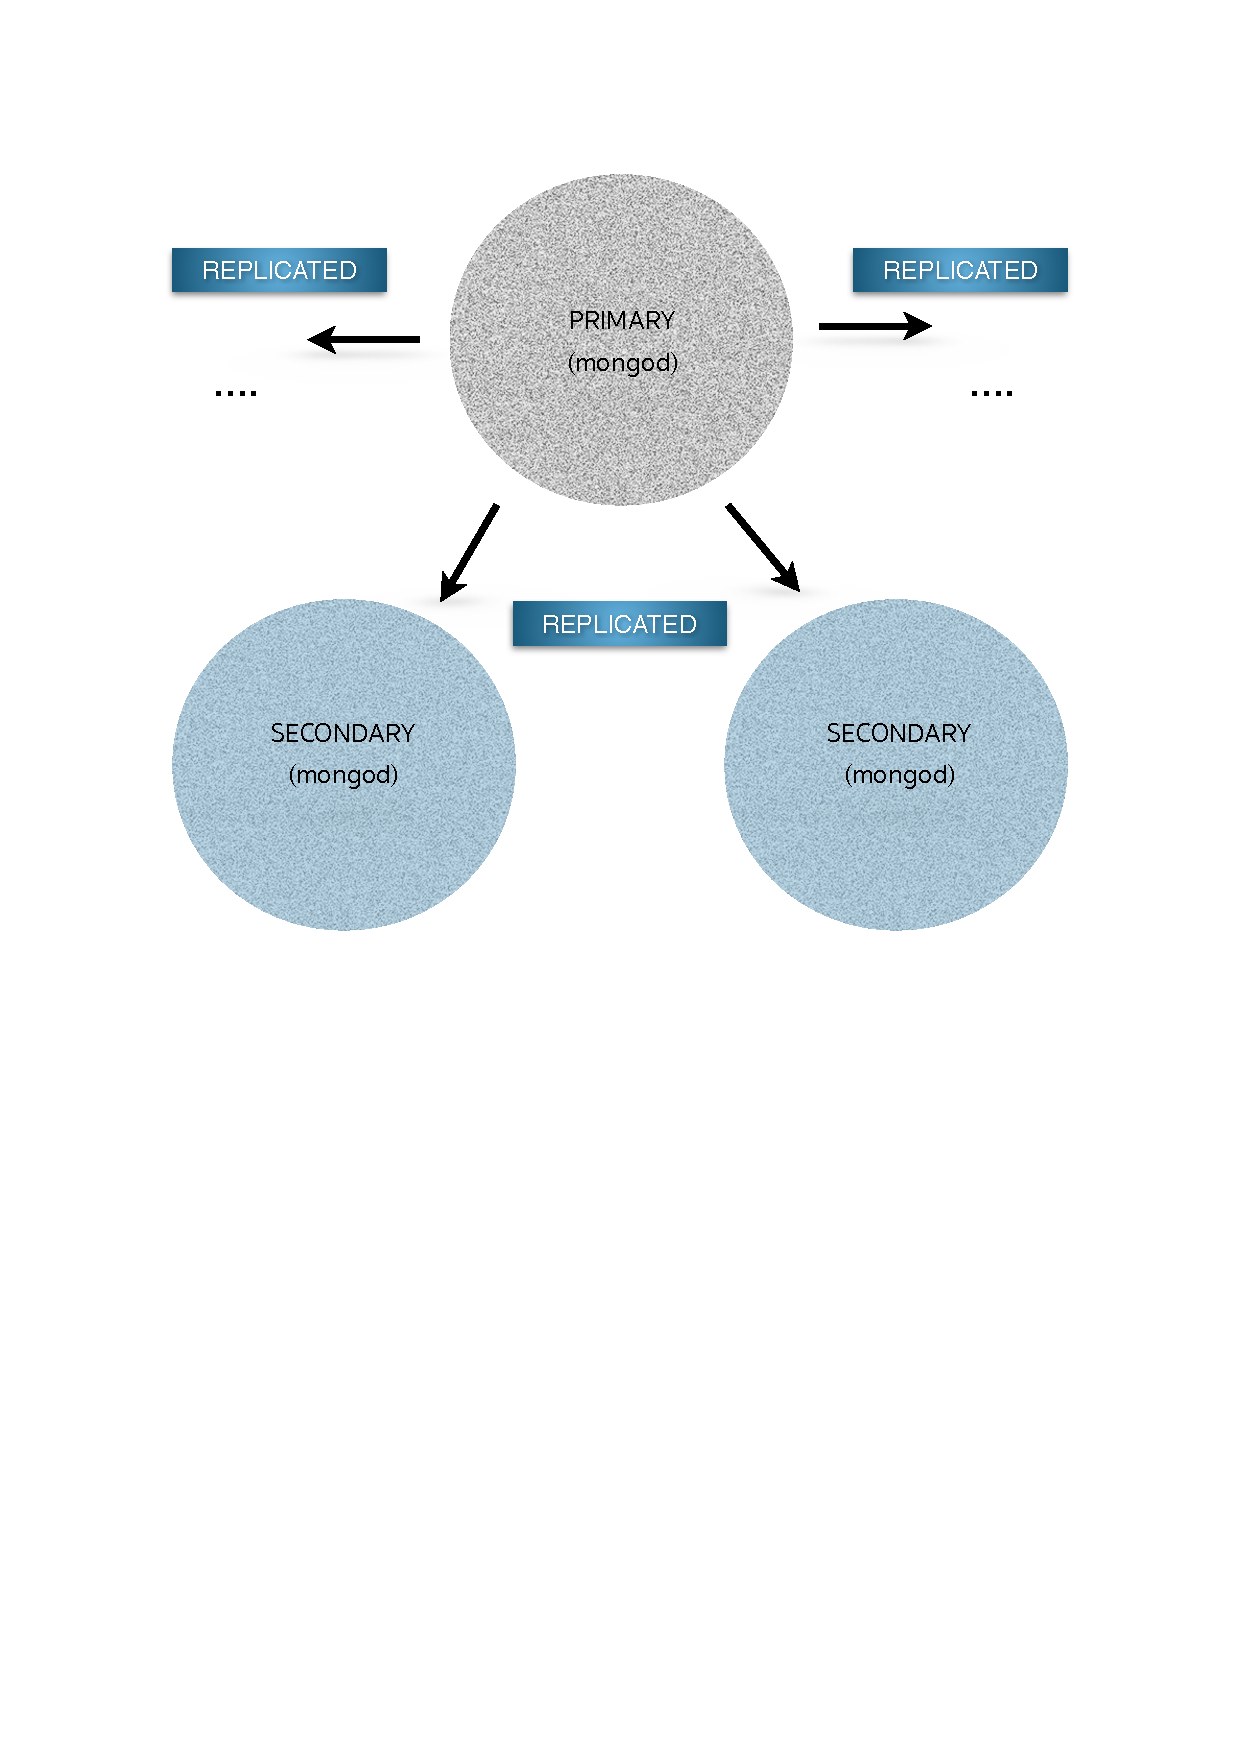
\includegraphics[trim = 28mm 139mm 28mm 29mm, clip, width=0.9\textwidth]{resources/replicaSet/createReplicaSet2}
      \caption[Initialer Zustand des Replica Sets]{Initialer Zustand des Replica Sets}
      % \caption[Ein Beispiel für eine Replikationsgruppe]{Ein Beispiel für eine Replikationsgruppe}
      \label{img:createReplicaSet}
   \end{subfigure}\hfill%
   \begin{subfigure}[t]{0.49\textwidth}\vspace{0pt}
   \centering
      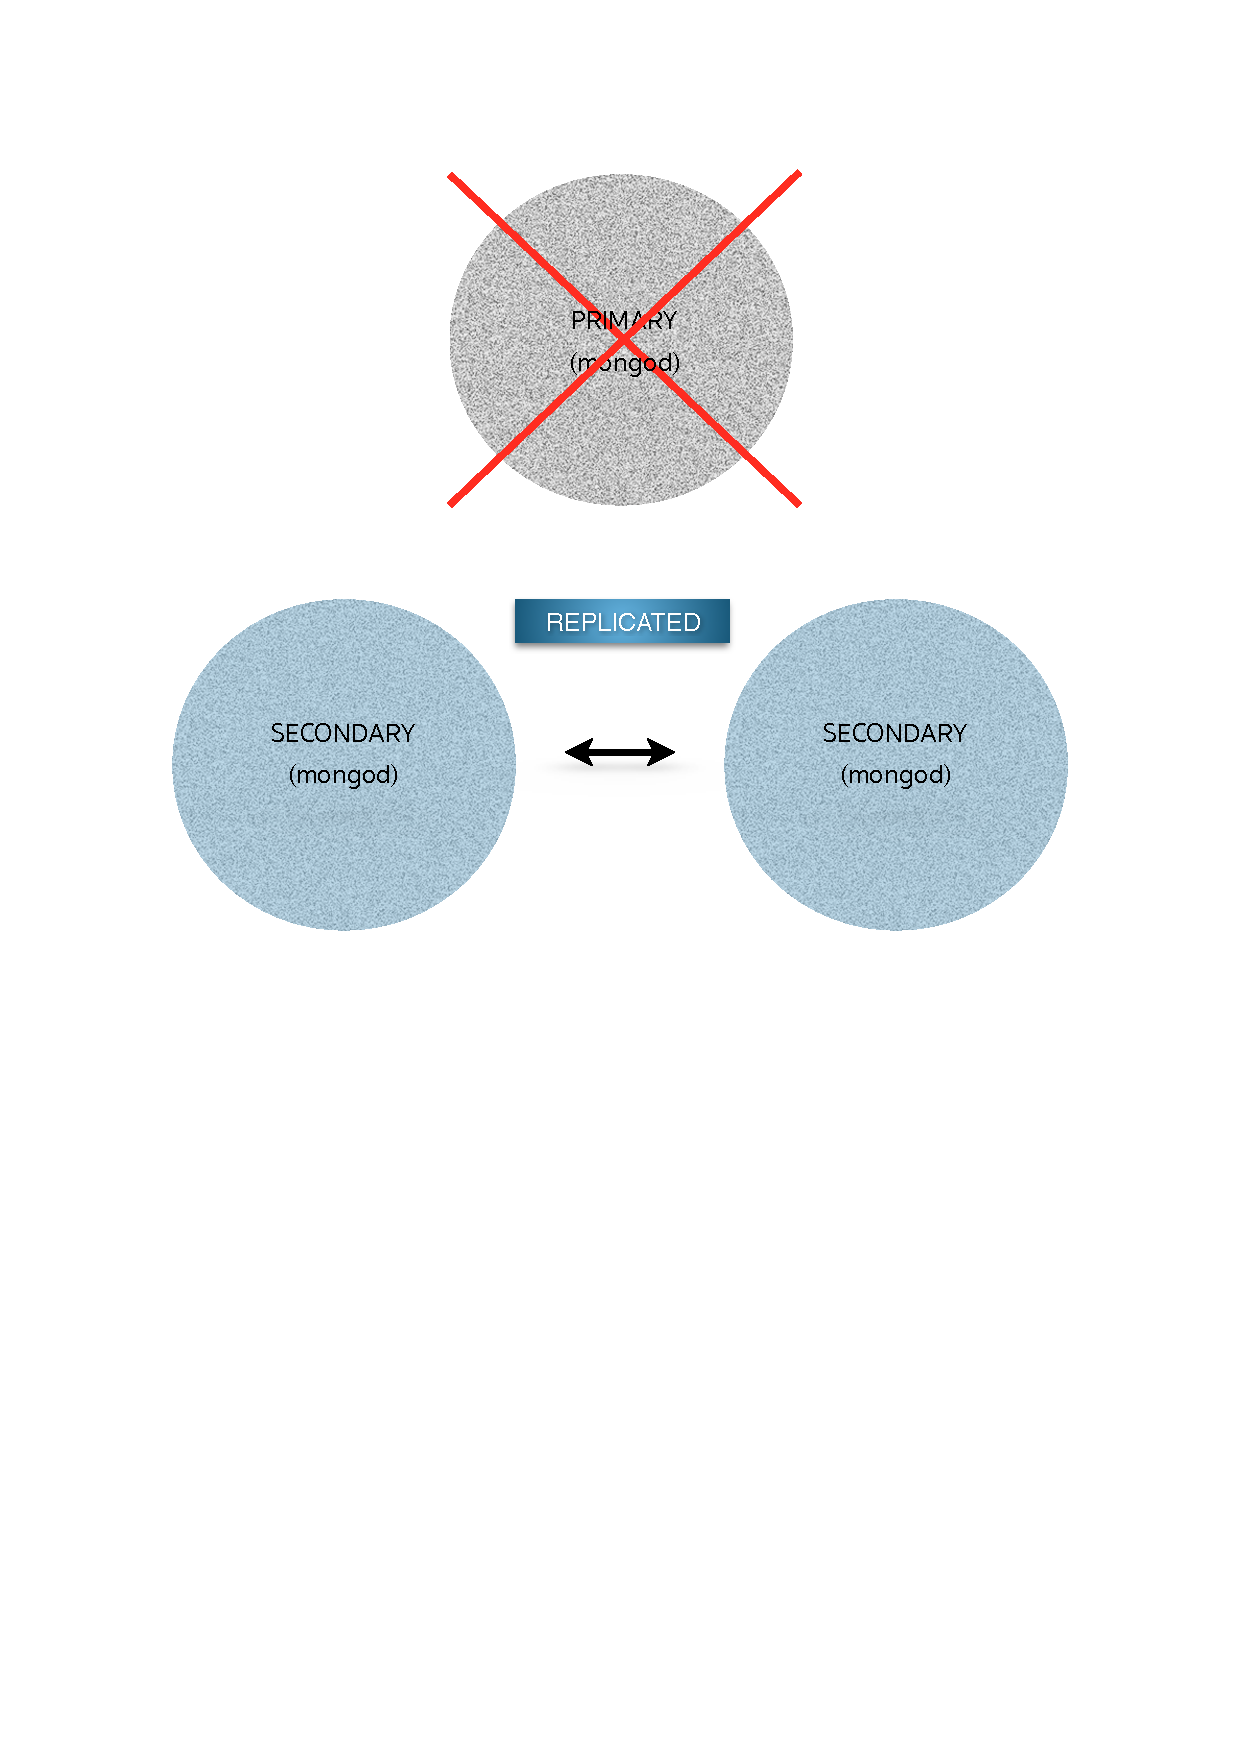
\includegraphics[trim = 28mm 139mm 28mm 29mm, clip, width=0.9\textwidth]{resources/replicaSet/selectNewPrimary}
     \caption[Ausfall des \textbf{Primary}-Knotens]{Ausfall des \textbf{Primary}-Knotens}
      \label{img:selectNewPrimary}
   \end{subfigure}\\[5pt]%
   \centering
   \begin{subfigure}[t]{0.49\textwidth}\vspace{0pt}
   \centering
        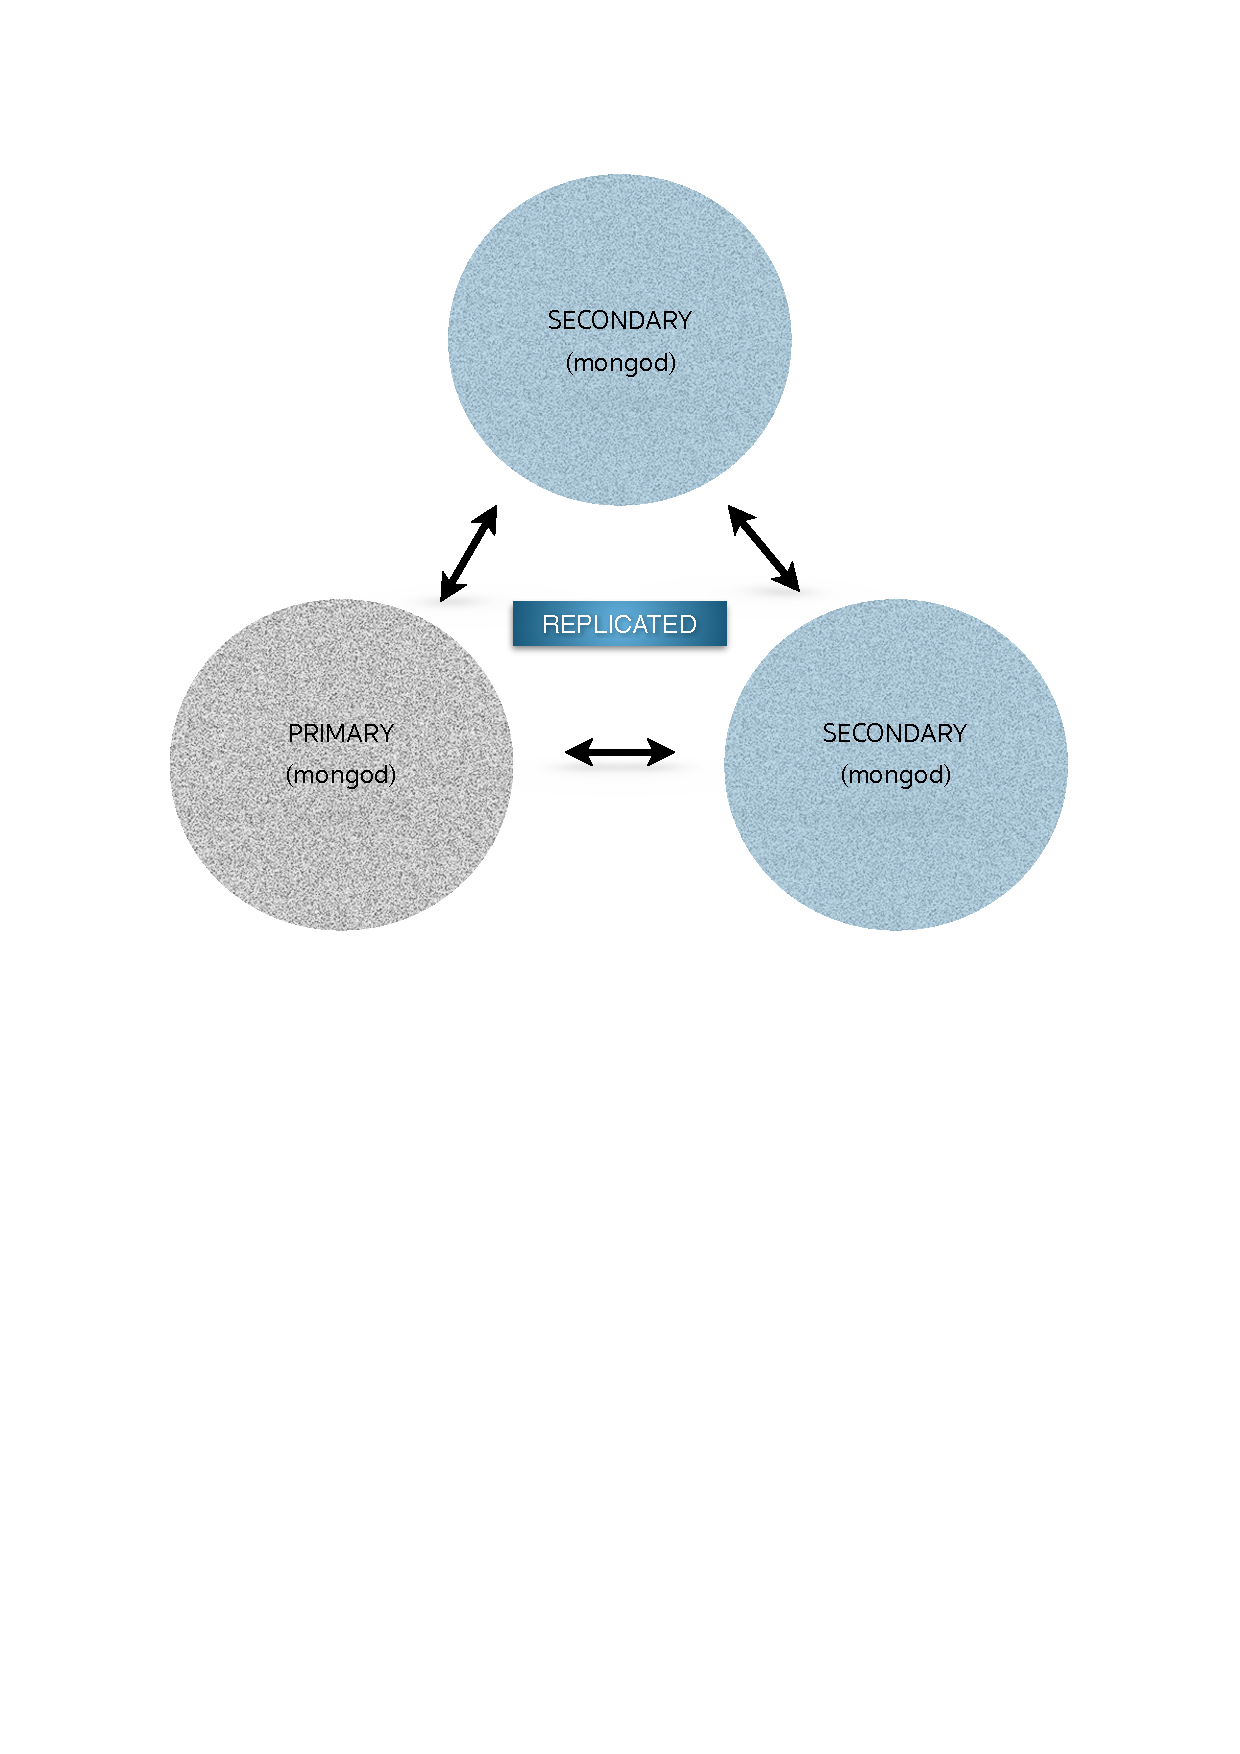
\includegraphics[trim = 28mm 139mm 28mm 29mm, clip, width=0.9\textwidth]{resources/replicaSet/newReplicaSet}
      \caption[Neuer \textbf{Primary} wurde gewählt]{Neuer \textbf{Primary} wurde gewählt}
      \label{img:newReplicaSet}
   \end{subfigure}
   \caption{Szenario für eine Replikationsgruppe mit drei Servern in einer \textit{Shard}}
   \label{img:replicaSetSzenario}
\end{figure}
Ein \textit{Master}, auch ein \textit{Primary} genannt, besitzt Schreib- und Leserechte. Dieser repliziert die Daten auf \textit{n-Slaves}, die auch als \textit{Secondaries} bezeichnet werden. Ein \textit{Primary} mit \textit{n-Secondaries} bilden gemeinsam eine \textit{Shard}. Eine \textit{Shard} kann aus mind. einem Server bestehen. Falls eine \textit{Shard} aus mehreren Servern besteht, so kann \mongo\ die Server in Replikationsgruppe \textit{(Replica set)} anordnen, damit bei Ausfall eines Servers die Verfügbarkeit der Datenbank trotzdem gewährleistet ist. Mit Replikationsgruppen will \mongo\ die Ausfallsicherheit sicherstellen. Die Abbildung \ref{img:replicaSetSzenario} veranschaulicht ein Szenario für eine Replikationsgruppe mit drei Knoten. Jeder Knoten aus der Gruppe ist als einen eigenen Server vorzustellen. %Das \textit{Master-n-Slaves-Prinzip} besagt, dass in einer Replikationsgruppe nur ein Master und n-Slaves existieren können, um eine strenge Konsistenz gewährleisten zu können. 
%\begin{figure}[H]
%\centering
%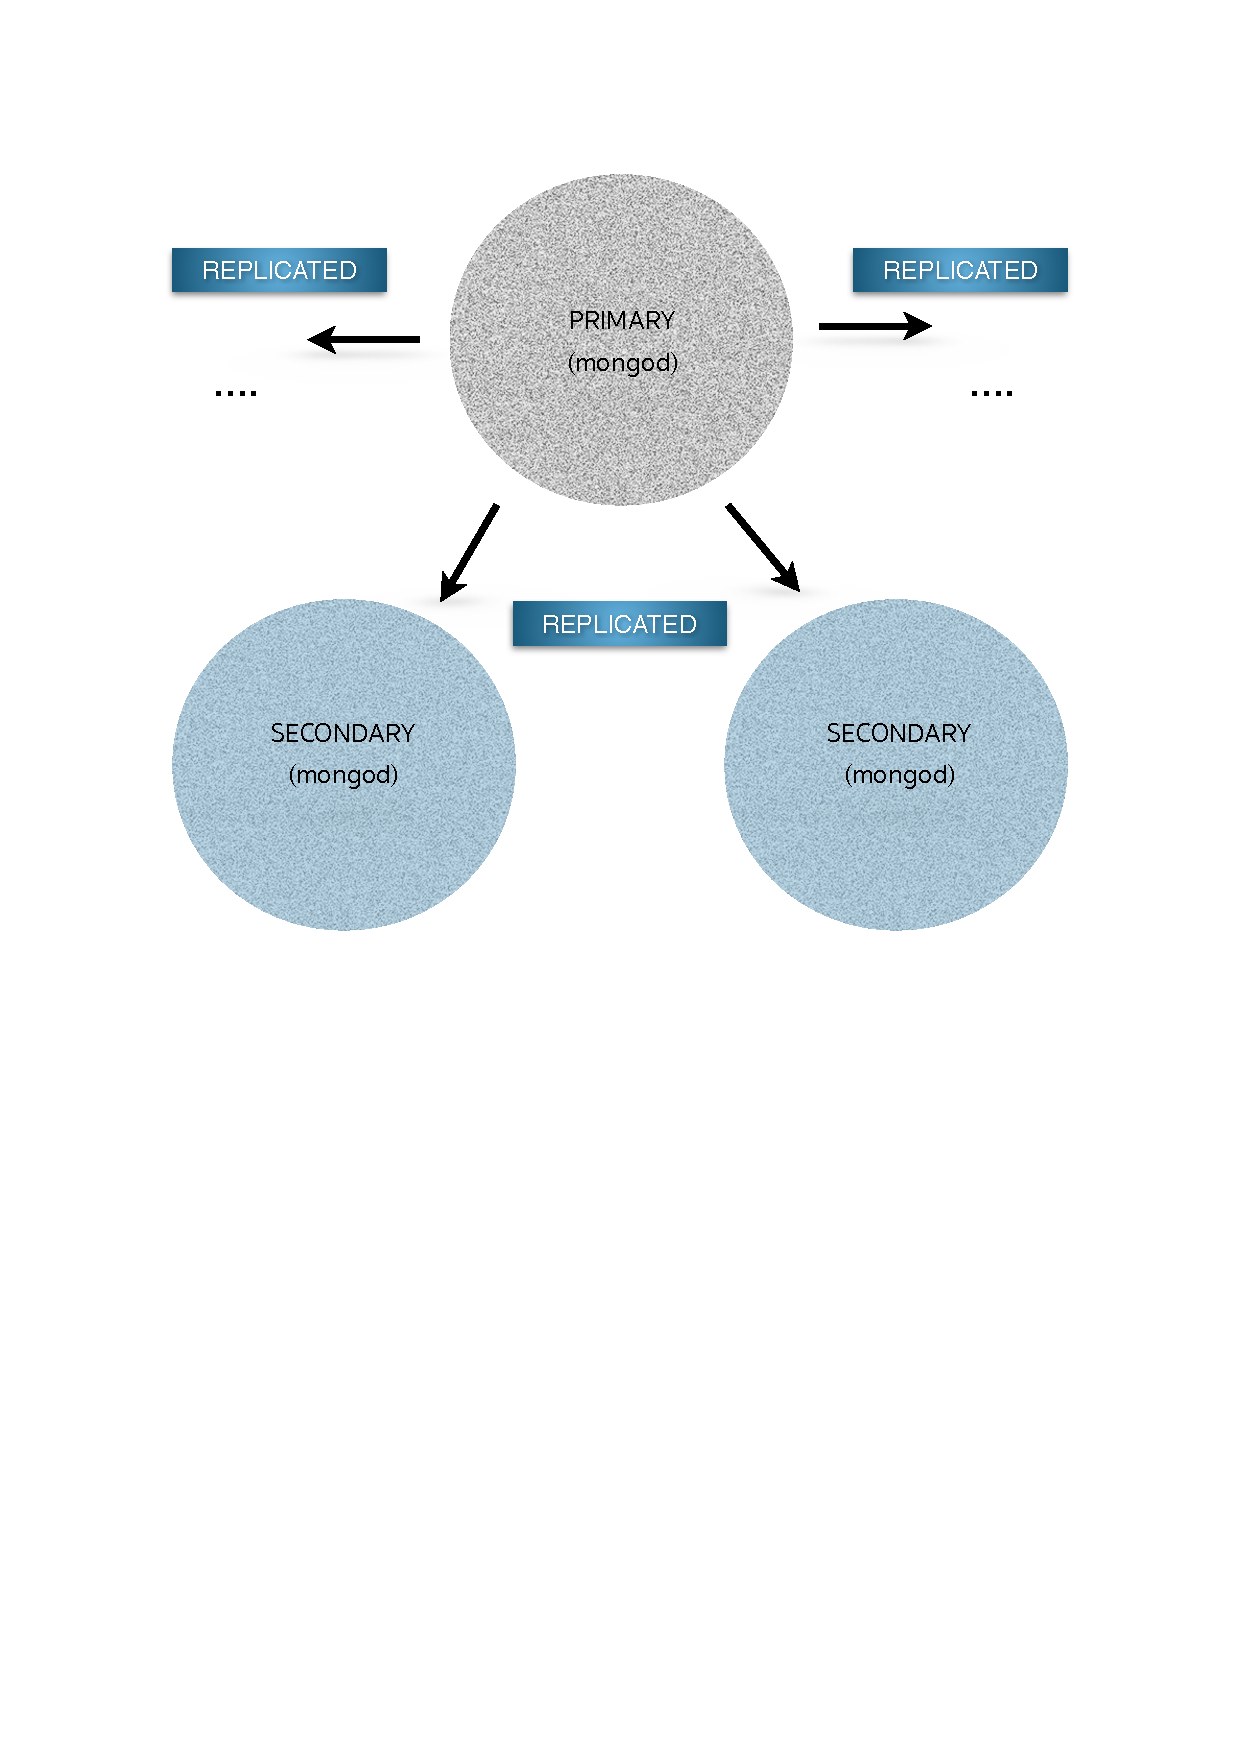
\includegraphics[trim = 0mm 139mm 0mm 28mm, clip, width=0.7\textwidth]{resources/replicaSet/createReplicaSet2}
%\caption[Ein Beispiel für eine Replikationsgruppe]{Ein Beispiel für eine Replikationsgruppe}
%\label{img:createReplicaSet}
%\end{figure}

%\begin{figure}[H]
%\centering
%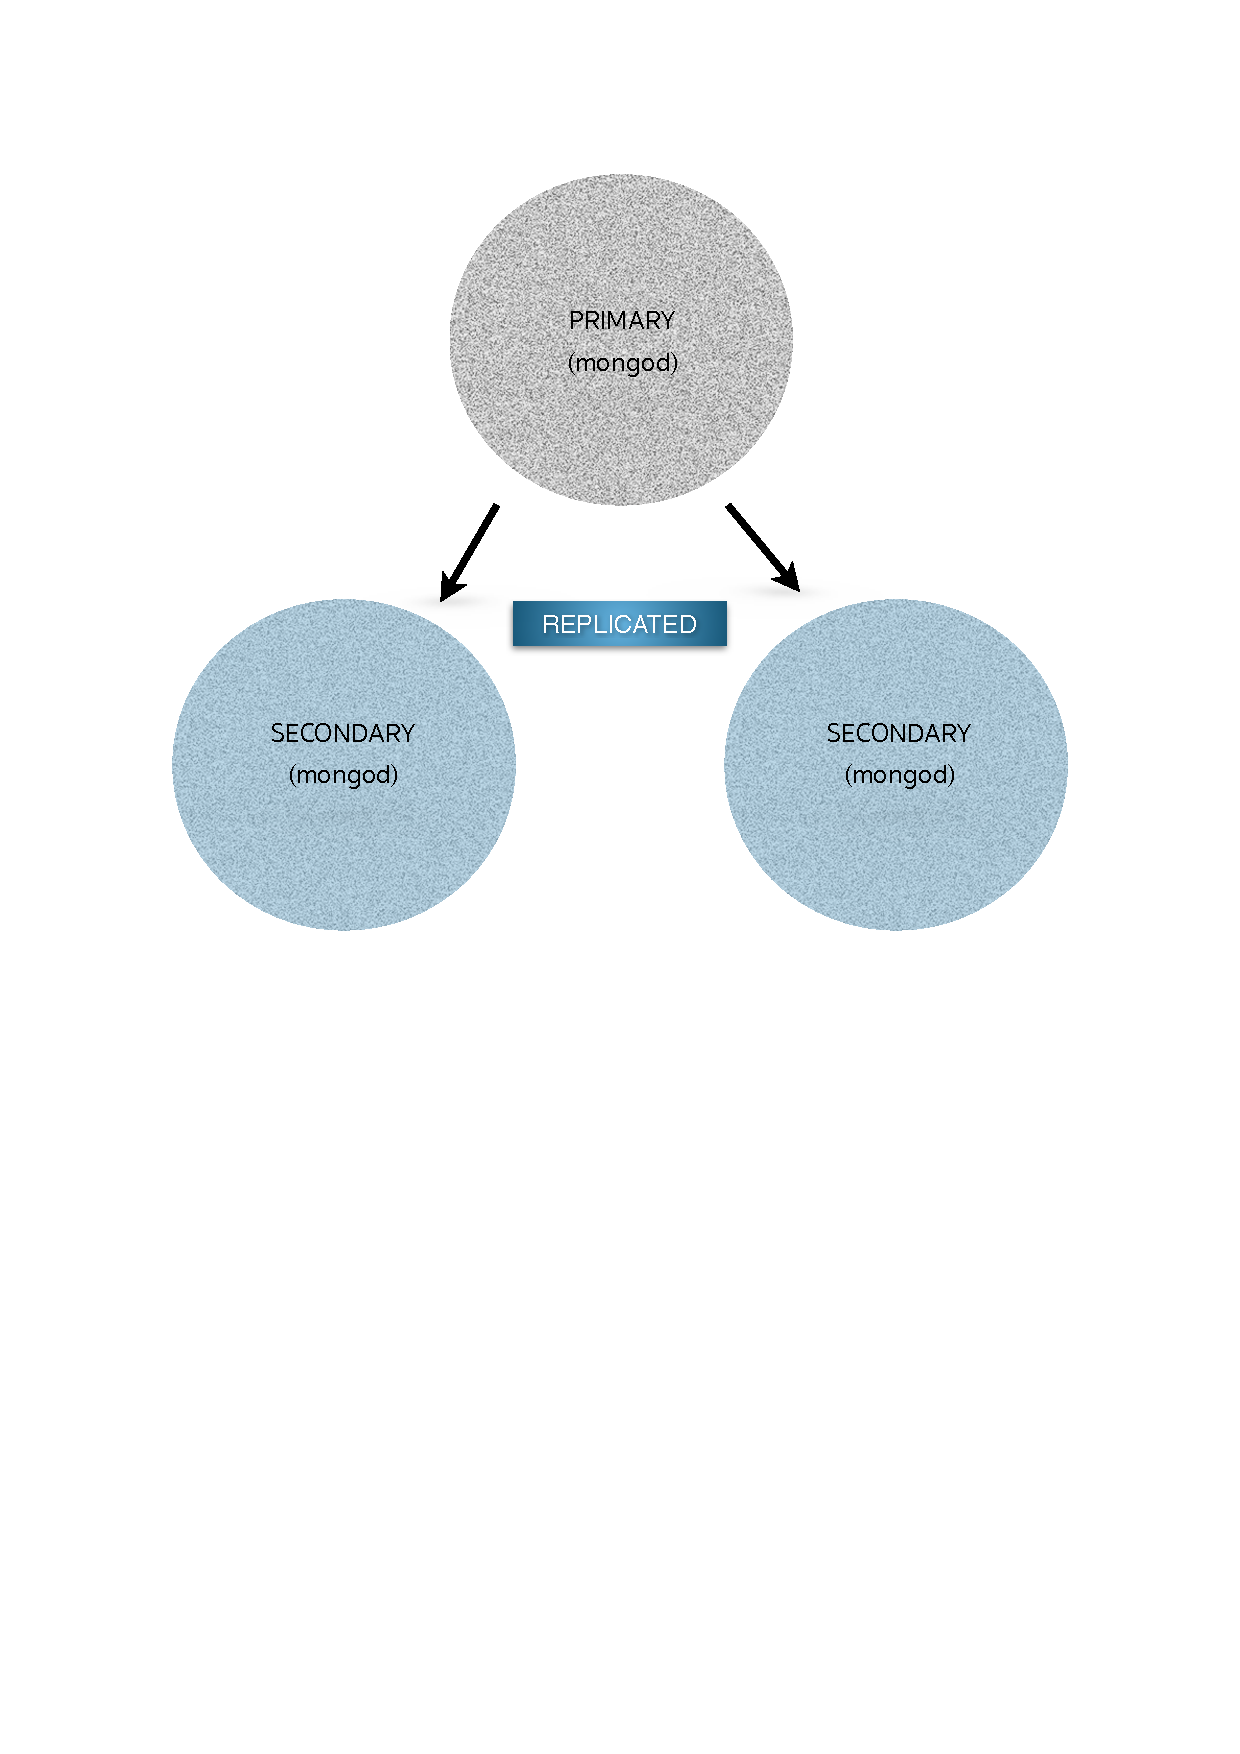
\includegraphics[trim = 0mm 139mm 0mm 9mm, clip, width=0.7\textwidth]{resources/replicaSet/createReplicaSet}
%\caption[Eine Replikationsgruppe mit einem Master und n-Slaves erzeugen]{Eine Replikationsgruppe mit einem Master und n-Slaves erzeugen}
%\label{img:createReplicaSet}
%\end{figure}
\begin{figure}[H]
   \begin{subfigure}[t]{0.49\textwidth}\vspace{0pt}
   \centering
    	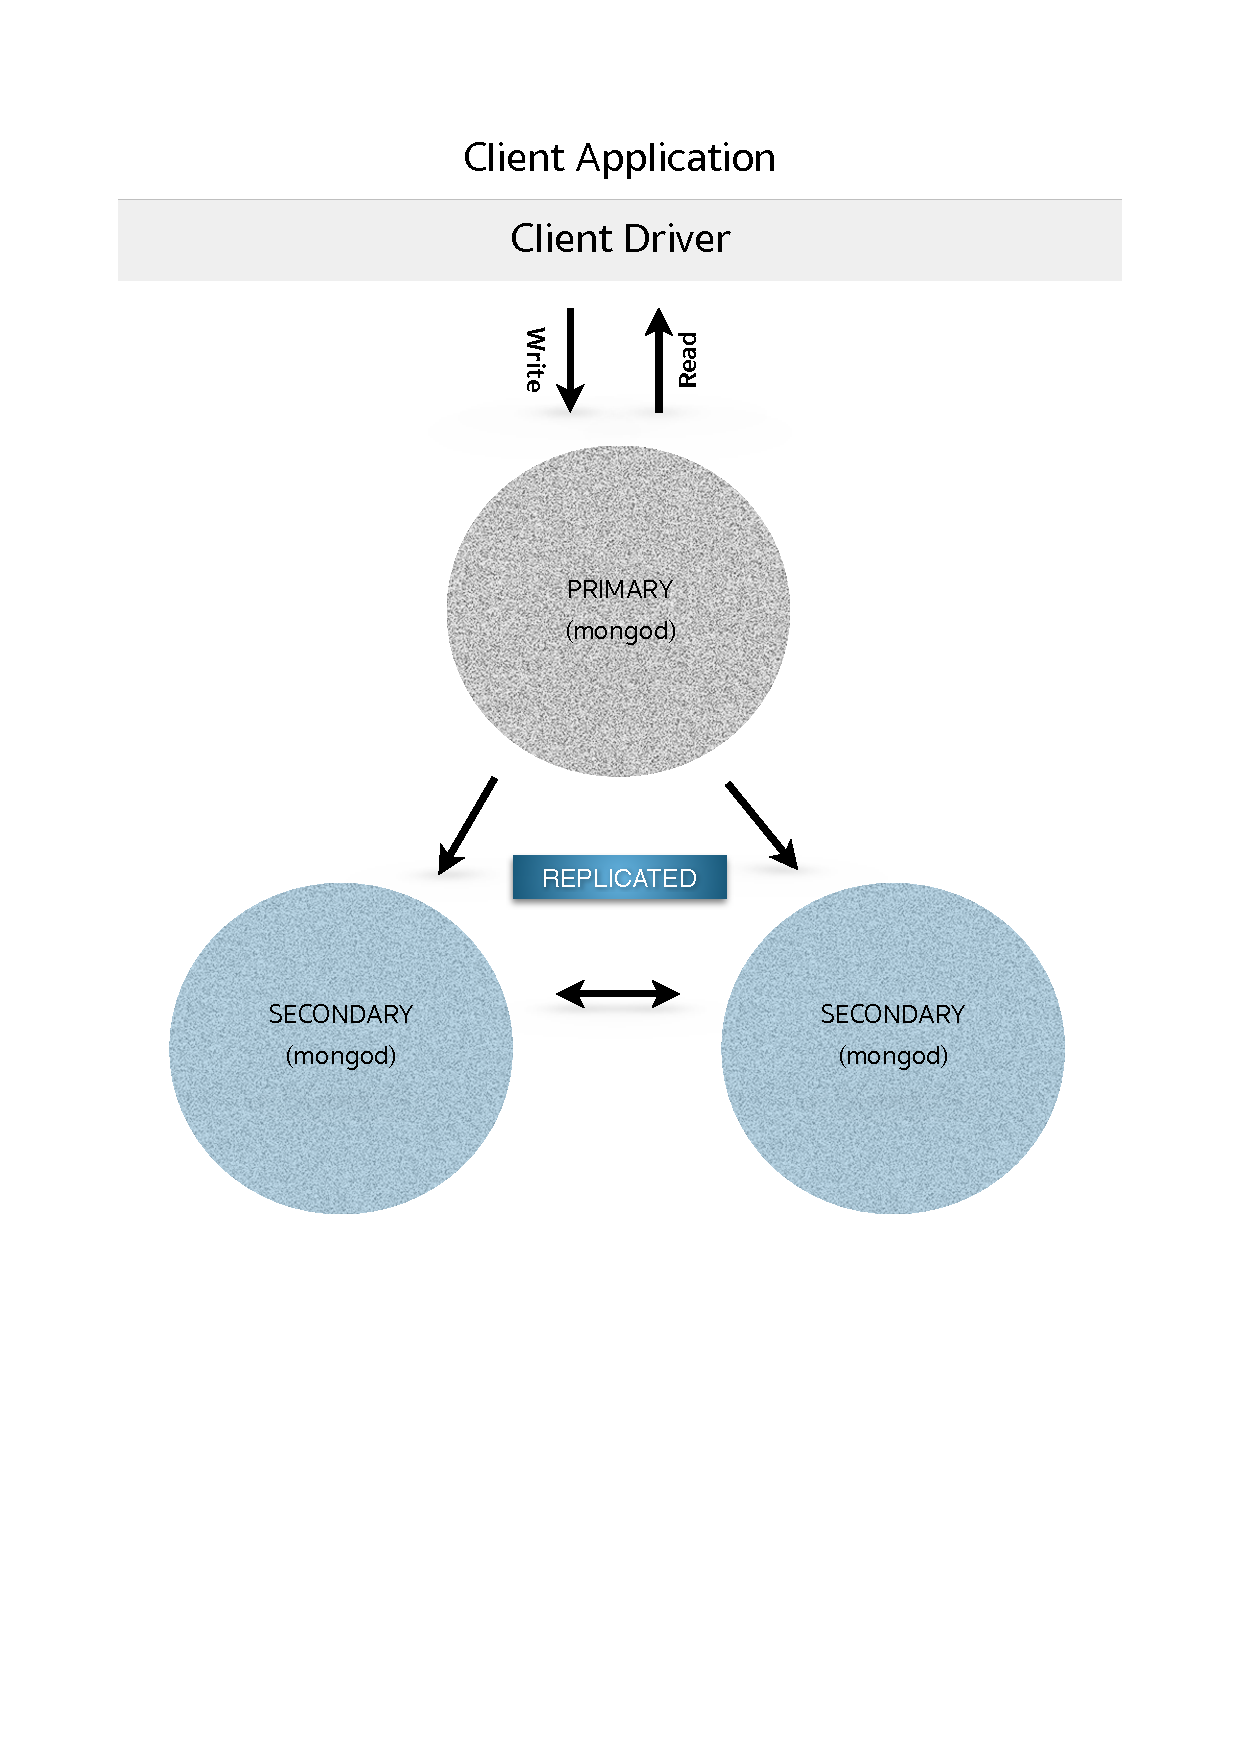
\includegraphics[trim = 0mm 90mm 0mm 20mm, clip, width=1.0\textwidth]{resources/replicaSet/replicaSetStrongConsistency}
	\caption[Lesezugriffe nur über Primary möglich]{Lesezugriffe nur über \textbf{Primary} möglich}
	\label{img:slaveNotOk}
   \end{subfigure}\hfill%
   \begin{subfigure}[t]{0.49\textwidth}\vspace{0pt}
   \centering
	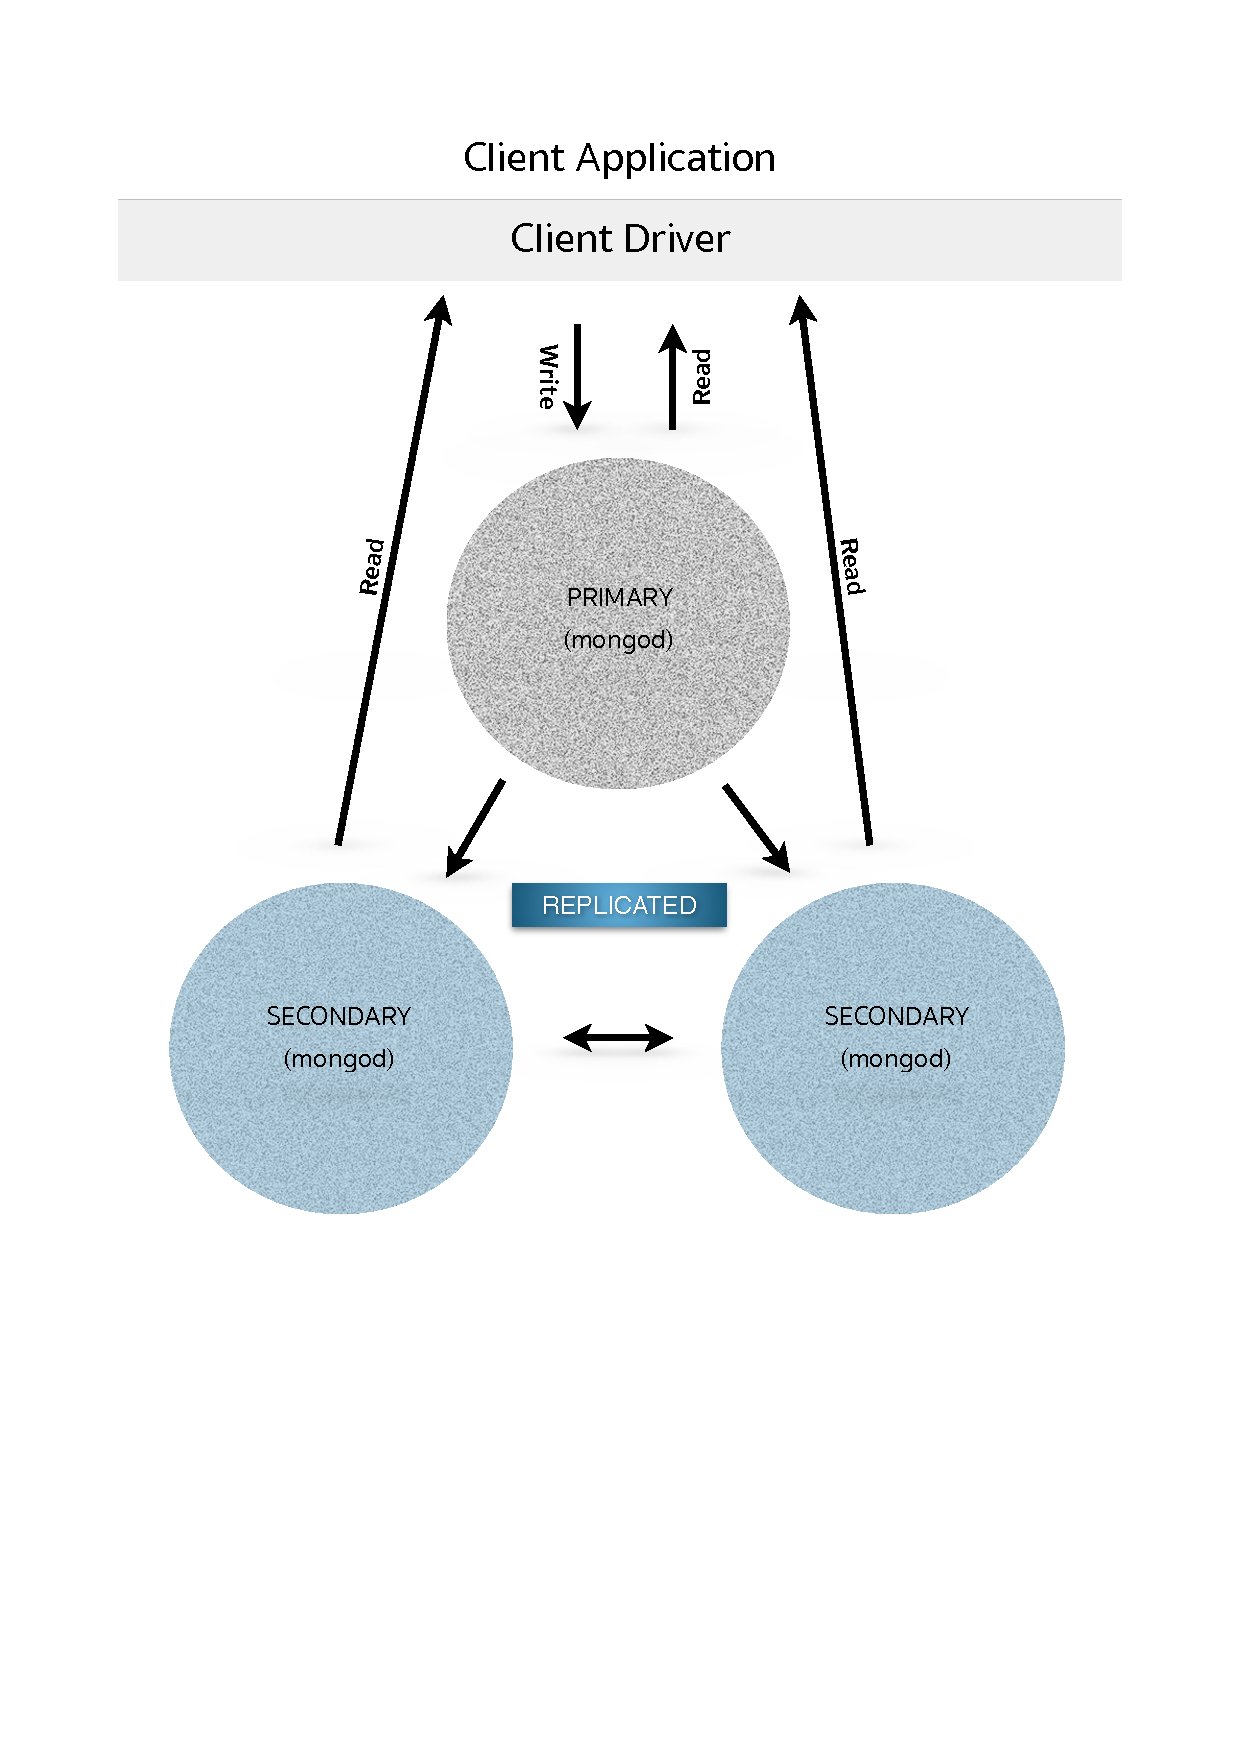
\includegraphics[trim = 0mm 90mm 0mm 20mm, clip, width=1.0\textwidth]{resources/replicaSet/eventualConsistency}
	\caption[Lesezugriffe auch über Secondaries freigeschaltet]{Lesezugriffe auch über \textbf{Secondaries} freigeschaltet}
	\label{img:slaveOk}
   \end{subfigure}\\[5pt]%
   \caption{Freischaltung der Lesezugriffe}
   \label{img:secondariesLowToRead}
\end{figure}
Im Gegenteil zu dem Primary sind bei Secondaries die Schreib- und Leserechte von Anfang an nicht möglich. Falls der Kontext der Anwendung verlangt, können nur die Leserechte auch bei Secondaries entsprechend freigeschaltet werden. Bei der Freischaltung der Leserrechte durch Secondaries muss jedoch in Kauf genommen werden, dass das Lesen durch Secondaries den konsistenten Zustand an Daten jedoch nicht garantiert. Der Grund dafür ist, dass die Schreiboperationen nur über den Master erfolgen und die Replikation der Daten etwas Zeit nimmt.

%\paragraph{\colorbox{yellow}{Horizontale Skalierung (Sharding)}}\label{sharding}
\paragraph{Horizontale Skalierung (Sharding)}\label{sharding}

Um eine kostengünstige Lösung für eine Steigerung der Leistung von Systemen zu ermöglichen, ermöglicht das Datenbanksystem von \mongo\  eine horizontale Skalierung. Die horizontale Verteilung der Daten erfolgt bei \mongo\ auf Ebene der \textit{Collections} nach \textit{Sharding-Keys}. Die \textit{Sharding-Keys} dienen dazu, um später Zugriffe auf einzelne Dokumente zu ermöglichen, die auf verschiedenen Servern abgelegt sind.
\begin{figure}[H]
\centering
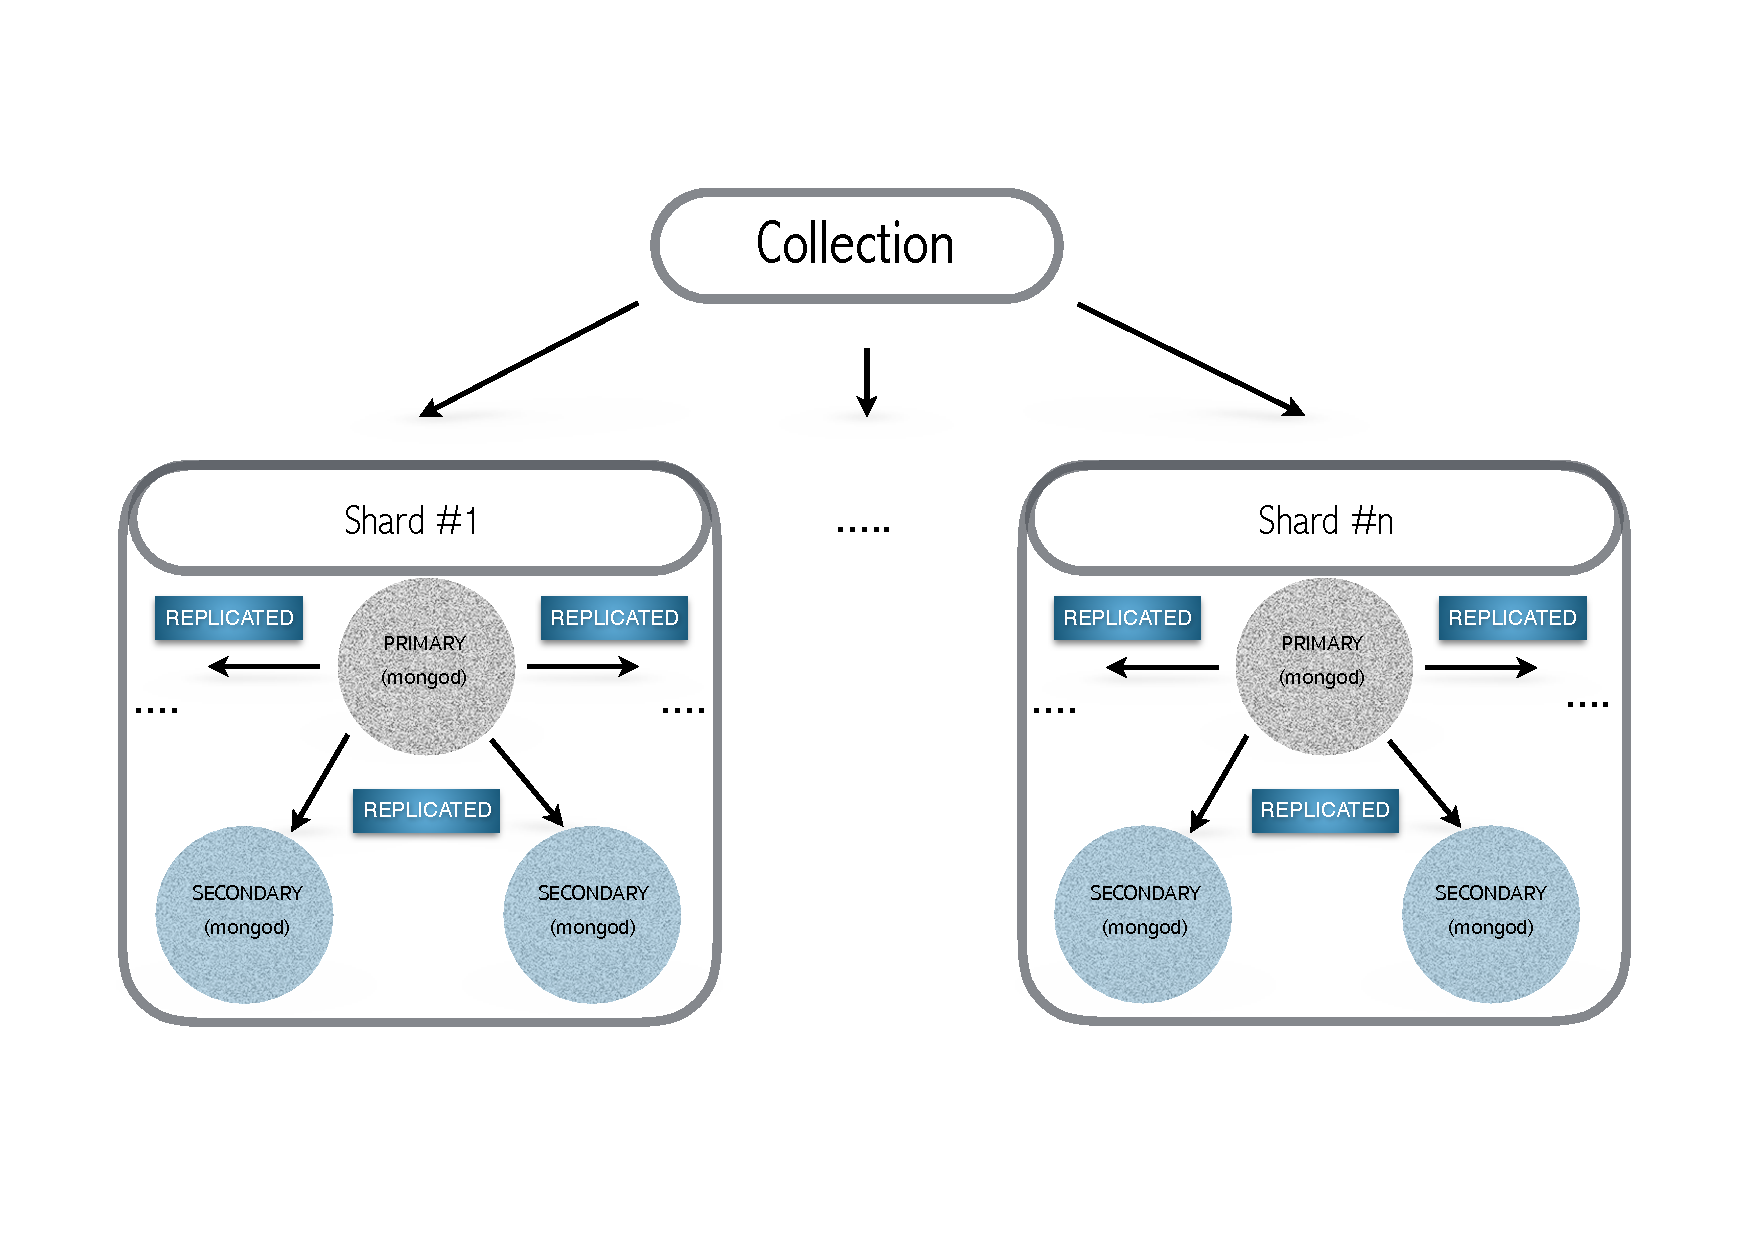
\includegraphics[trim = 0mm 35mm 0mm 30mm, clip, width=1.0\textwidth]{resources/replicaSet/sharding}
\caption[Ein Beispiel für Verteilung einer \textit{Collection} auf mehreren \textit{Shards}]{Ein Beispiel für Verteilung einer \textit{Collection} auf mehreren \textit{Shards}}
\label{img:sharding}
\end{figure}
Die Aufteilung der \textit{Collections} erfolgt in Blocks, auch als \textit{Chunks} genannt. Ein \textit{Chunk} ist ein Teil einer bestimmten \textit{Collection}. Gespeichert werden \textit{Chunks} auf Servern, die in diesem Zusammenhang als \textit{Shards} bezeichnet werden.

Um die Aufteilung der \textit{Collections} in \textit{Chunks} auf \textit{Shards} realisieren zu können, verwendet \mongo\ folgende Komponenten:
\begin{itemize}
\item \textit{shards:} Die \textit{Shards} enthalten letztendlich die Daten. In einer \textit{Shard} ist es möglich, Replikationsgruppen zu verwenden.
\item \textit{mongos:} Der \textit{mongos} gilt als ein \textit{RoutingService}, der die Anfragen der Anwendungsschicht entgegennimmt und diese an eine entsprechende \textit{Shard} weiterleitet, die die nötigen Daten enthält.
\item \textit{config servers:} Die Konfigurationsserver speichern die Metadaten für einen Sharded-Cluster. Im Fall einer Schreiboperation entscheiden die Konfigurationsserver, in welchen Chunk auf welchem Shard das entsprechende Dokument eingefügt wird. Bei der Leseoperation geben die Konfigurationsserver den Auskunft darüber, welcher Shard die gewünschten Daten enthält. Bei den Konfigurationsservern handeln es um eine \textit{mongod-}Instanzen.
\end{itemize}
Die Abbildung \ref{img:shardedCluster} veranschaulicht die Interaktion von den gerade genannten Komponenten innerhalb eines Sharded-Cluster:
%\colorbox{red}{graphische Darstellung}
\begin{figure}[H]
\centering
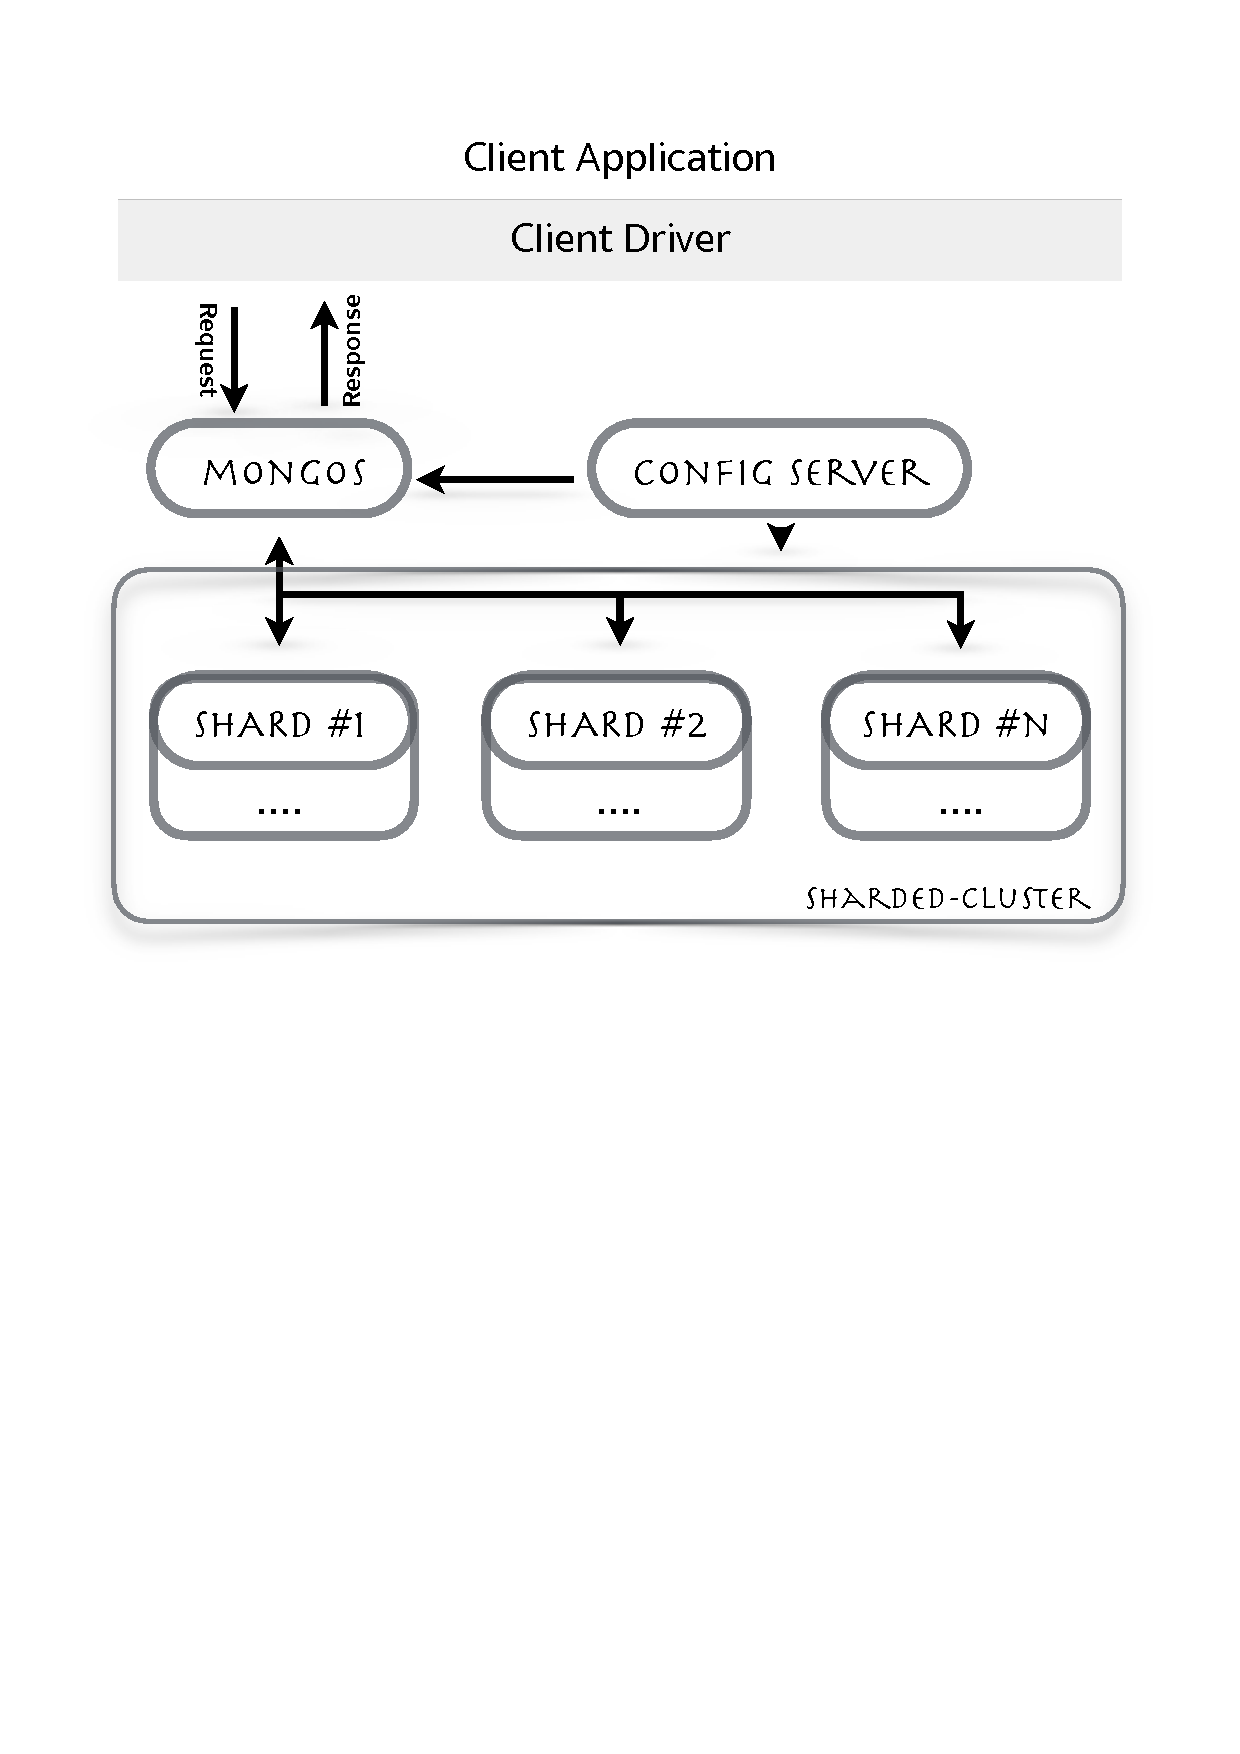
\includegraphics[trim = 0mm 139mm 0mm 22mm, clip, width=0.7\textwidth]{resources/replicaSet/shardedCluster}
\caption[Horizontale Skalierung \textit{(Sharding)}]{Horizontale Skalierung \textit{(Sharding)}}
\label{img:shardedCluster}
\end{figure}

Das Ziel des Ganzen ist die horizontale Skalierbarkeit an Datenmengen, um die Performance des Datenbanksystems zu steigern.

%\paragraph{\colorbox{yellow}{Fragmentierung nach \textit{Shard-Keys}}}\label{sharding-keys}
\paragraph{Fragmentierung nach \textit{Shard-Keys}}\label{sharding-keys}
Die Fragmentierung der Daten erfolgt auf Ebene der \textit{Collections} nach \textit{Shard-Keys}. In jeder \textit{Collection}  muss ein Schlüssel als sogenannter \textit{Sharding-Key} definiert sein, der entsprechend in jedem Dokument derselben \textit{Collection} existiert.  \textit{Sharding-Key} kann entweder aus einem einzigen indexierten Feld oder einem zusammengesetzten Index bestehen. Die Dokumente werden dann nach \textit{Shard-Key} alphabetisch oder nummerisch sortiert und anschließend in \textit{n-}Blocks gleicher Größe eingeteilt. \mongo\ garantiert die gleichmäßige Verteilung der Blocks an \textit{Shards}.
\begin{figure}[H]
\centering
%trim = links, unten, rechts, oben
 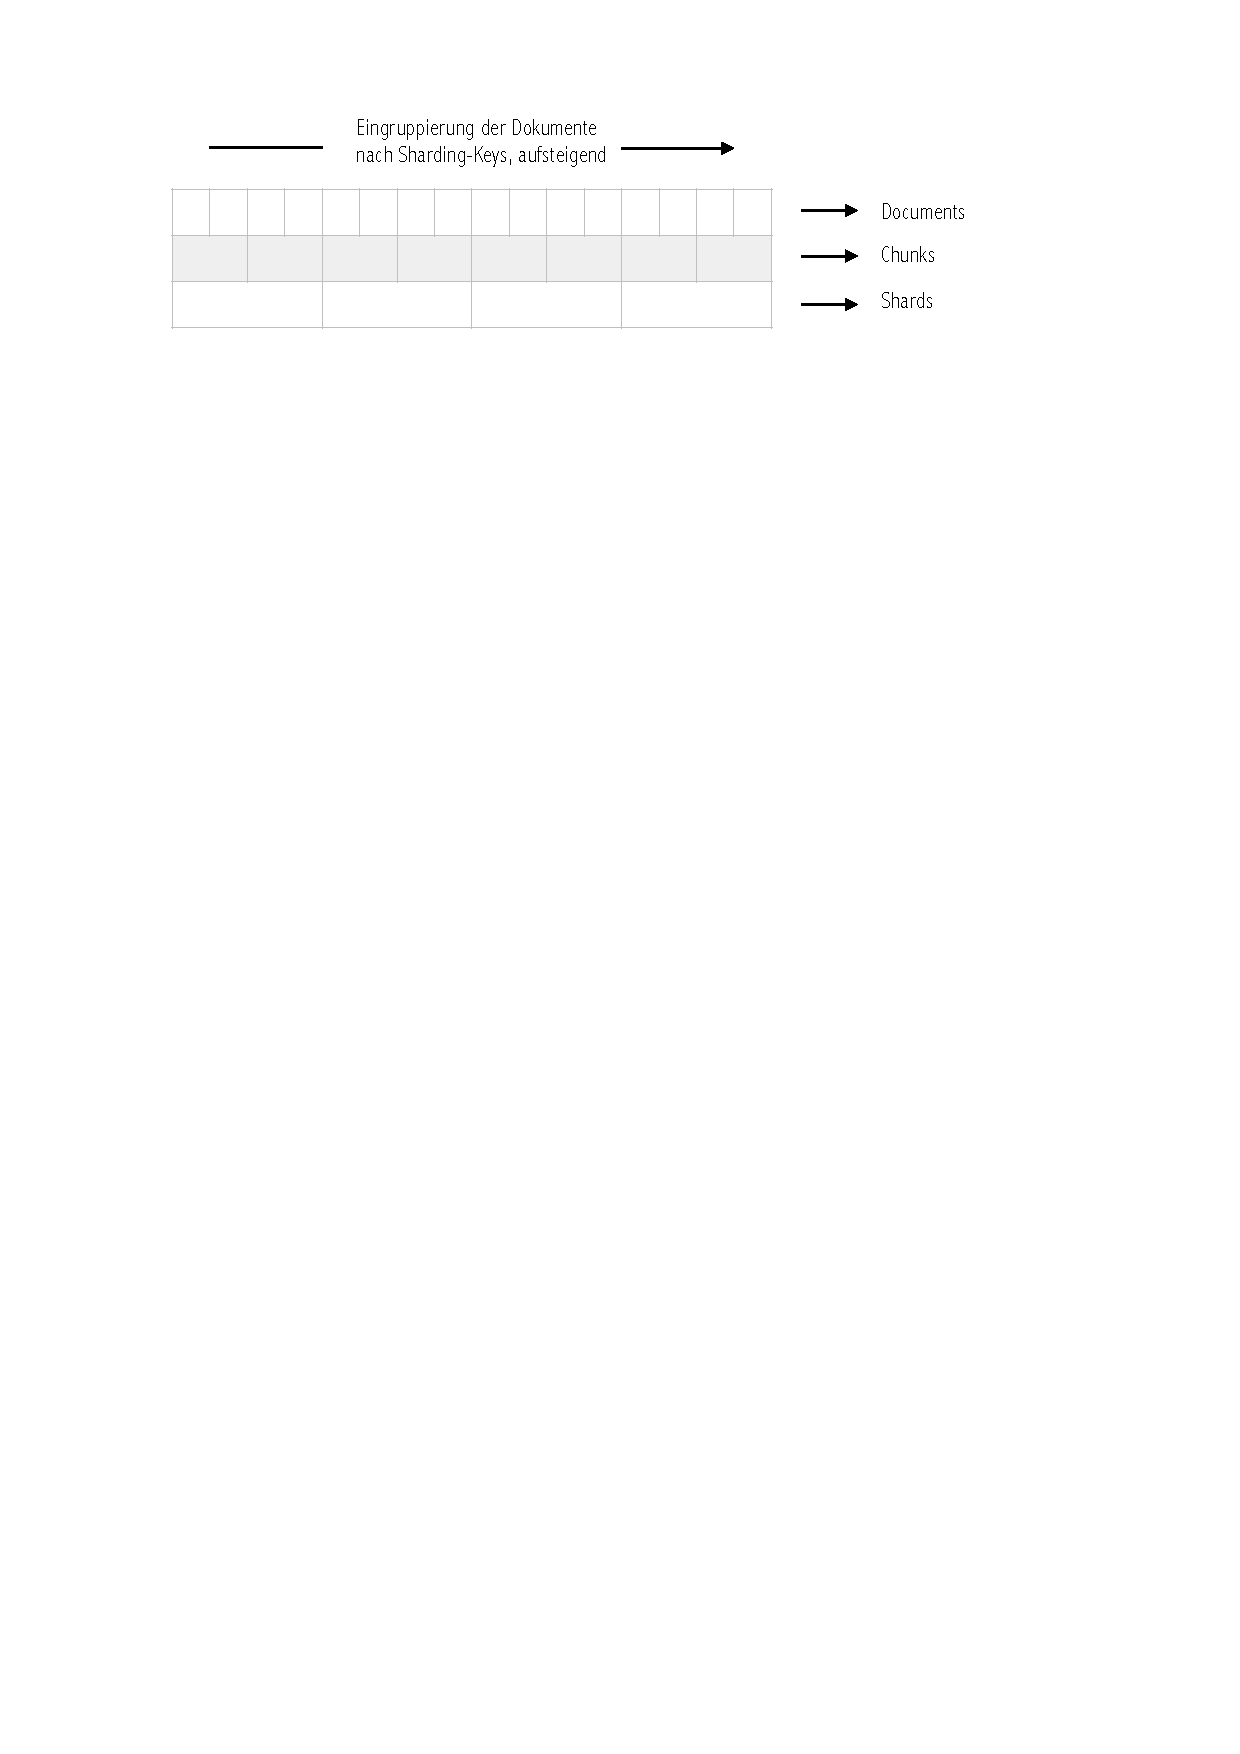
\includegraphics[trim = 25mm 240mm 40mm 20mm, clip, width=0.9\textwidth]{resources/replicaSet/sharding-keys}
\caption[Anordnung der Dokumente in Blocks (=\textit{Chunks}) unter Verwendung des \textit{Shard-Keys}. Mehrere Blocks bilden dementsprechend eine \textit{Shard}.]{Anordnung der Dokumente in Blocks (=\textit{Chunks}) unter Verwendung des \textit{Shard-Keys}. Mehrere Blocks bilden dementsprechend eine \textit{Shard}.}
\label{img:shardKeys}
\end{figure}

Bei der \textit{Shard-Keys} Konfiguration müssen folgende \textit{Constraints\footnote{Introduction to Sharding: \url{https://www.mongodb.com/presentations/back-to-basics-4-introduction-to-sharding?p=589c5c940aca4c55041426f1&utm_campaign=Int_WB_Back\%20to\%20Basics\%20Series\%20\%28English\%29_01_17_EMEA\%20-\%20Follow\%20Up\%204&utm_medium=email&utm_source=Eloqua}, zugegriffen am 2. Februar 2017}} berücksichtigt werden:
\begin{itemize}
\item \textit{Shard-Keys} sind unabänderlich
\item \textit{Shard-Keys} verfügen über eine hohe Kardinalität
\item \textit{Shard-Keys} sind eindeutig
\item \textit{Shard-Keys} existiert dann in jedem Dokument
\item \textit{Shard-Keys} ist bis zum 512 bytes limitiert
\item \textit{Shard-Keys} ist es nicht möglich, als Multi-Key zu bilden
\end{itemize}

%\begin{figure}[H]
%\centering
%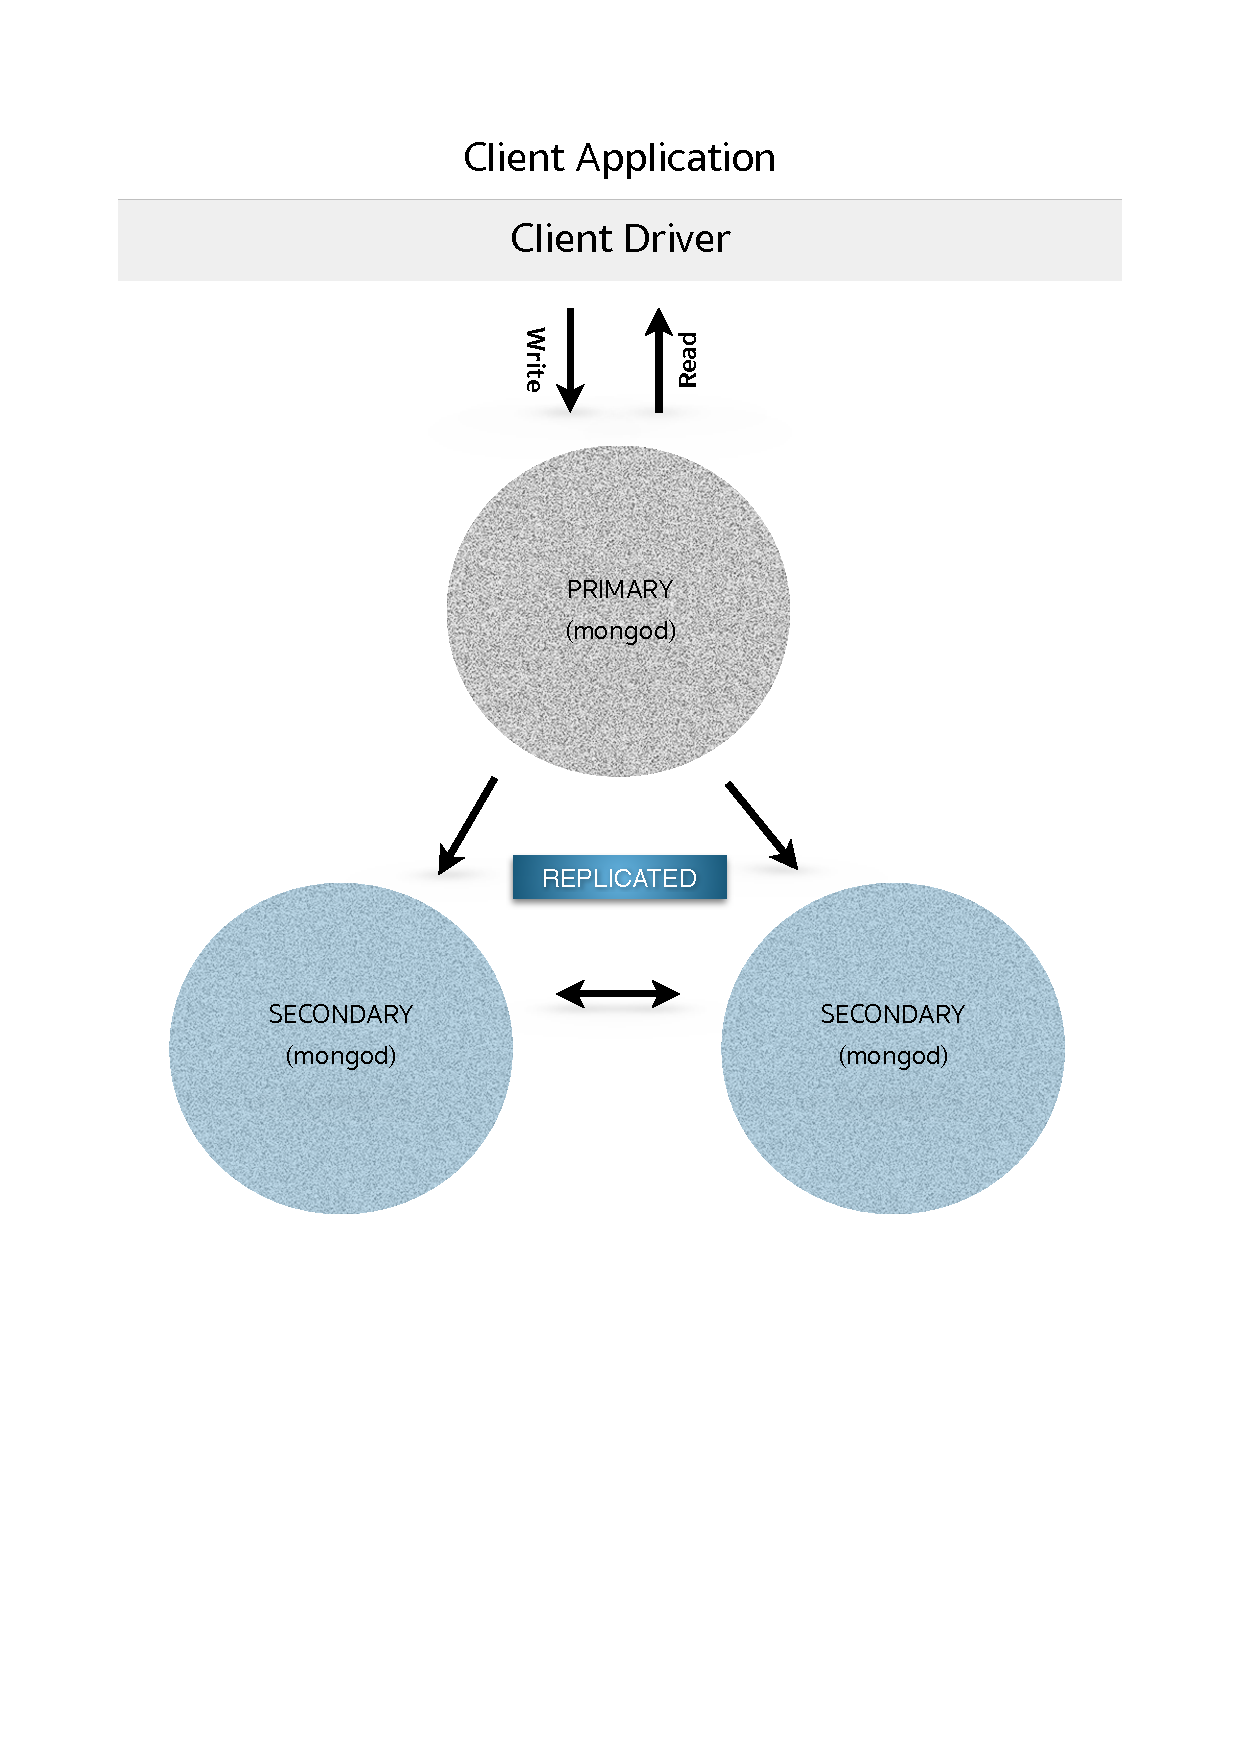
\includegraphics[trim = 0mm 90mm 0mm 20mm, clip, width=0.7\textwidth]{resources/replicaSet/replicaSetStrongConsistency}
%\caption[Lesezugriffe nur über Primary möglich]{Lesezugriffe nur über \textbf{Primary} möglich}
%\label{img:slaveNotOk}
%\end{figure}
%
%\begin{figure}[H]
%\centering
%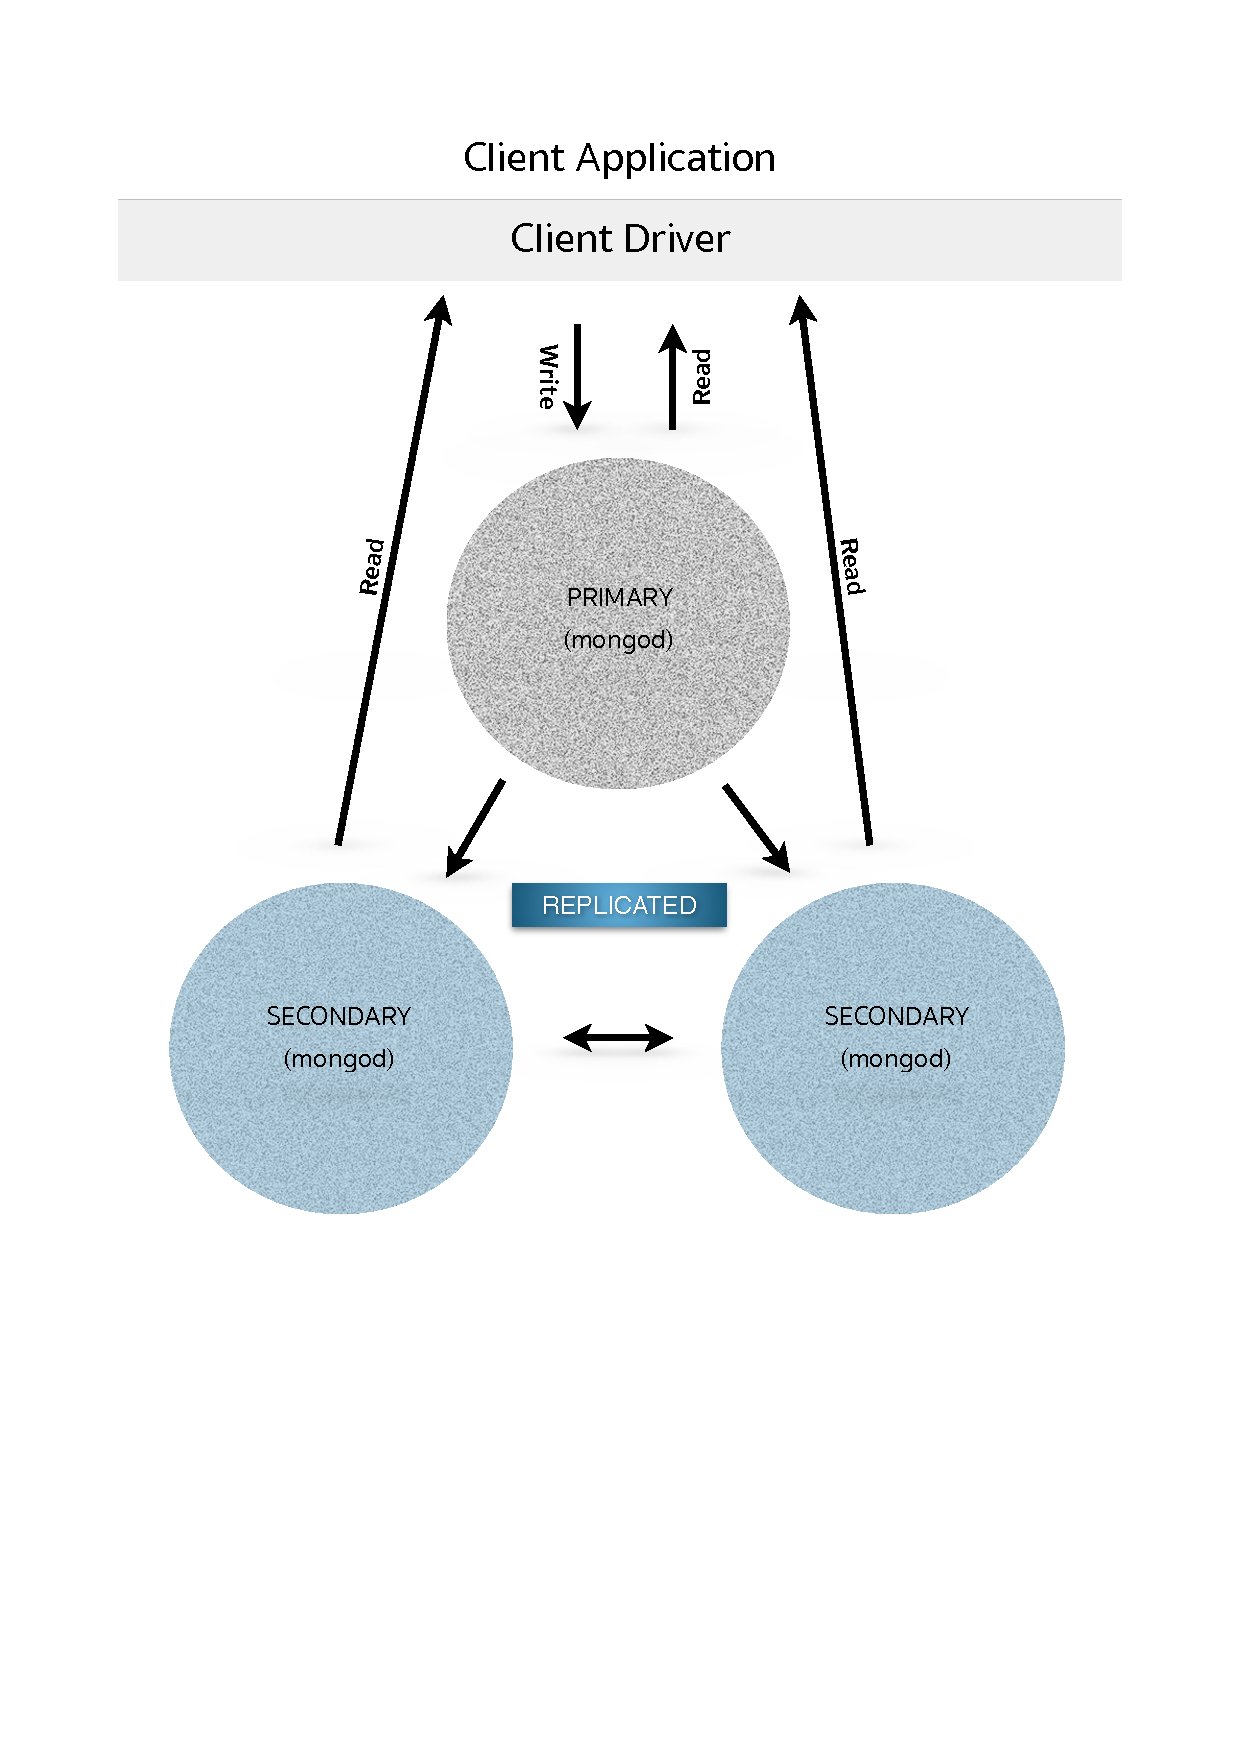
\includegraphics[trim = 0mm 90mm 0mm 20mm, clip, width=0.7\textwidth]{resources/replicaSet/eventualConsistency}
%\caption[Lesezugriffe auch über Secondaries freigeschaltet]{Lesezugriffe auch über \textbf{Secondaries} freigeschaltet}
%\label{img:slaveOk}
%\end{figure}

%\begin{figure}[H]
%\centering
%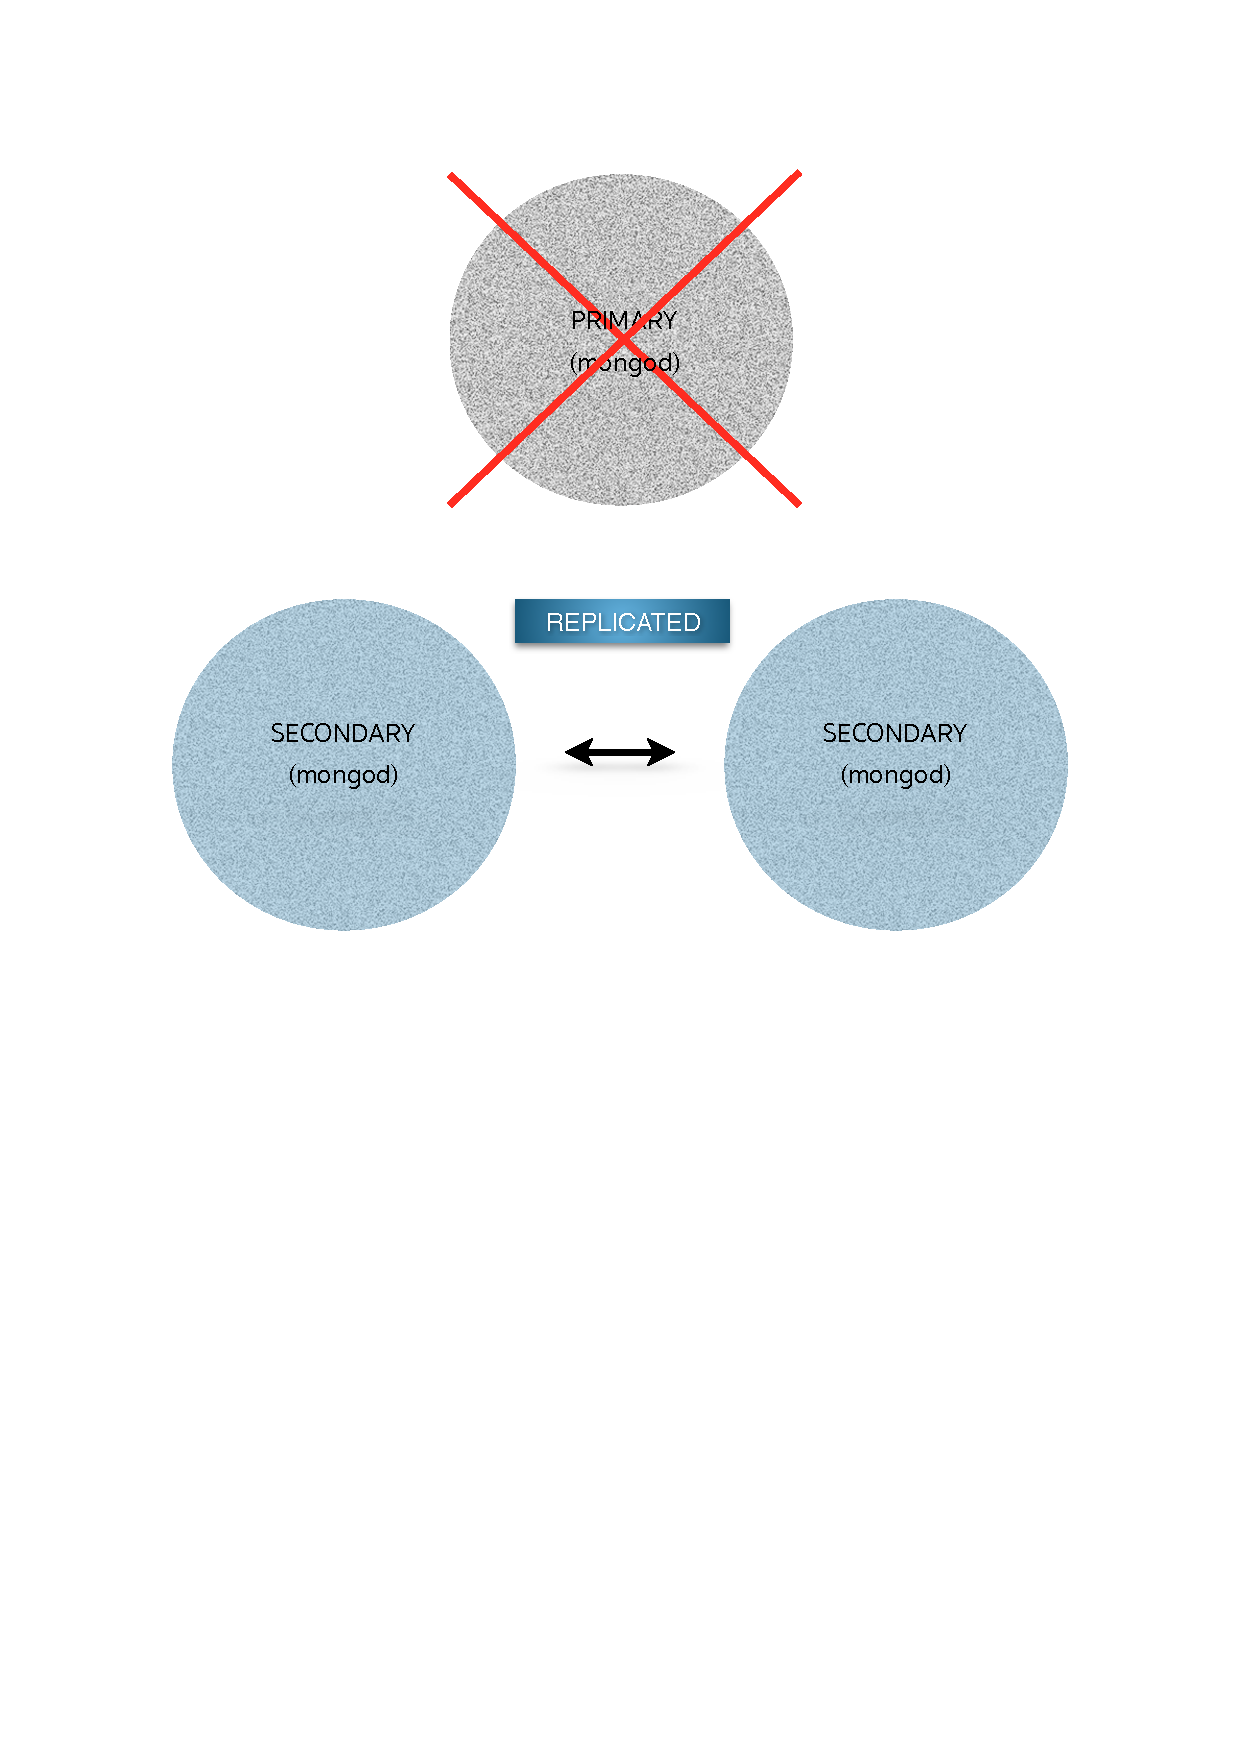
\includegraphics[trim = 0mm 139mm 0mm 28mm, clip, width=0.7\textwidth]{resources/replicaSet/selectNewPrimary}
%\caption[\textbf{Primary} fehlte aus]{\textbf{Primary} fehlte aus}
%\label{img:selectNewPrimary}
%\end{figure}

%\begin{figure}[H]
%\centering
%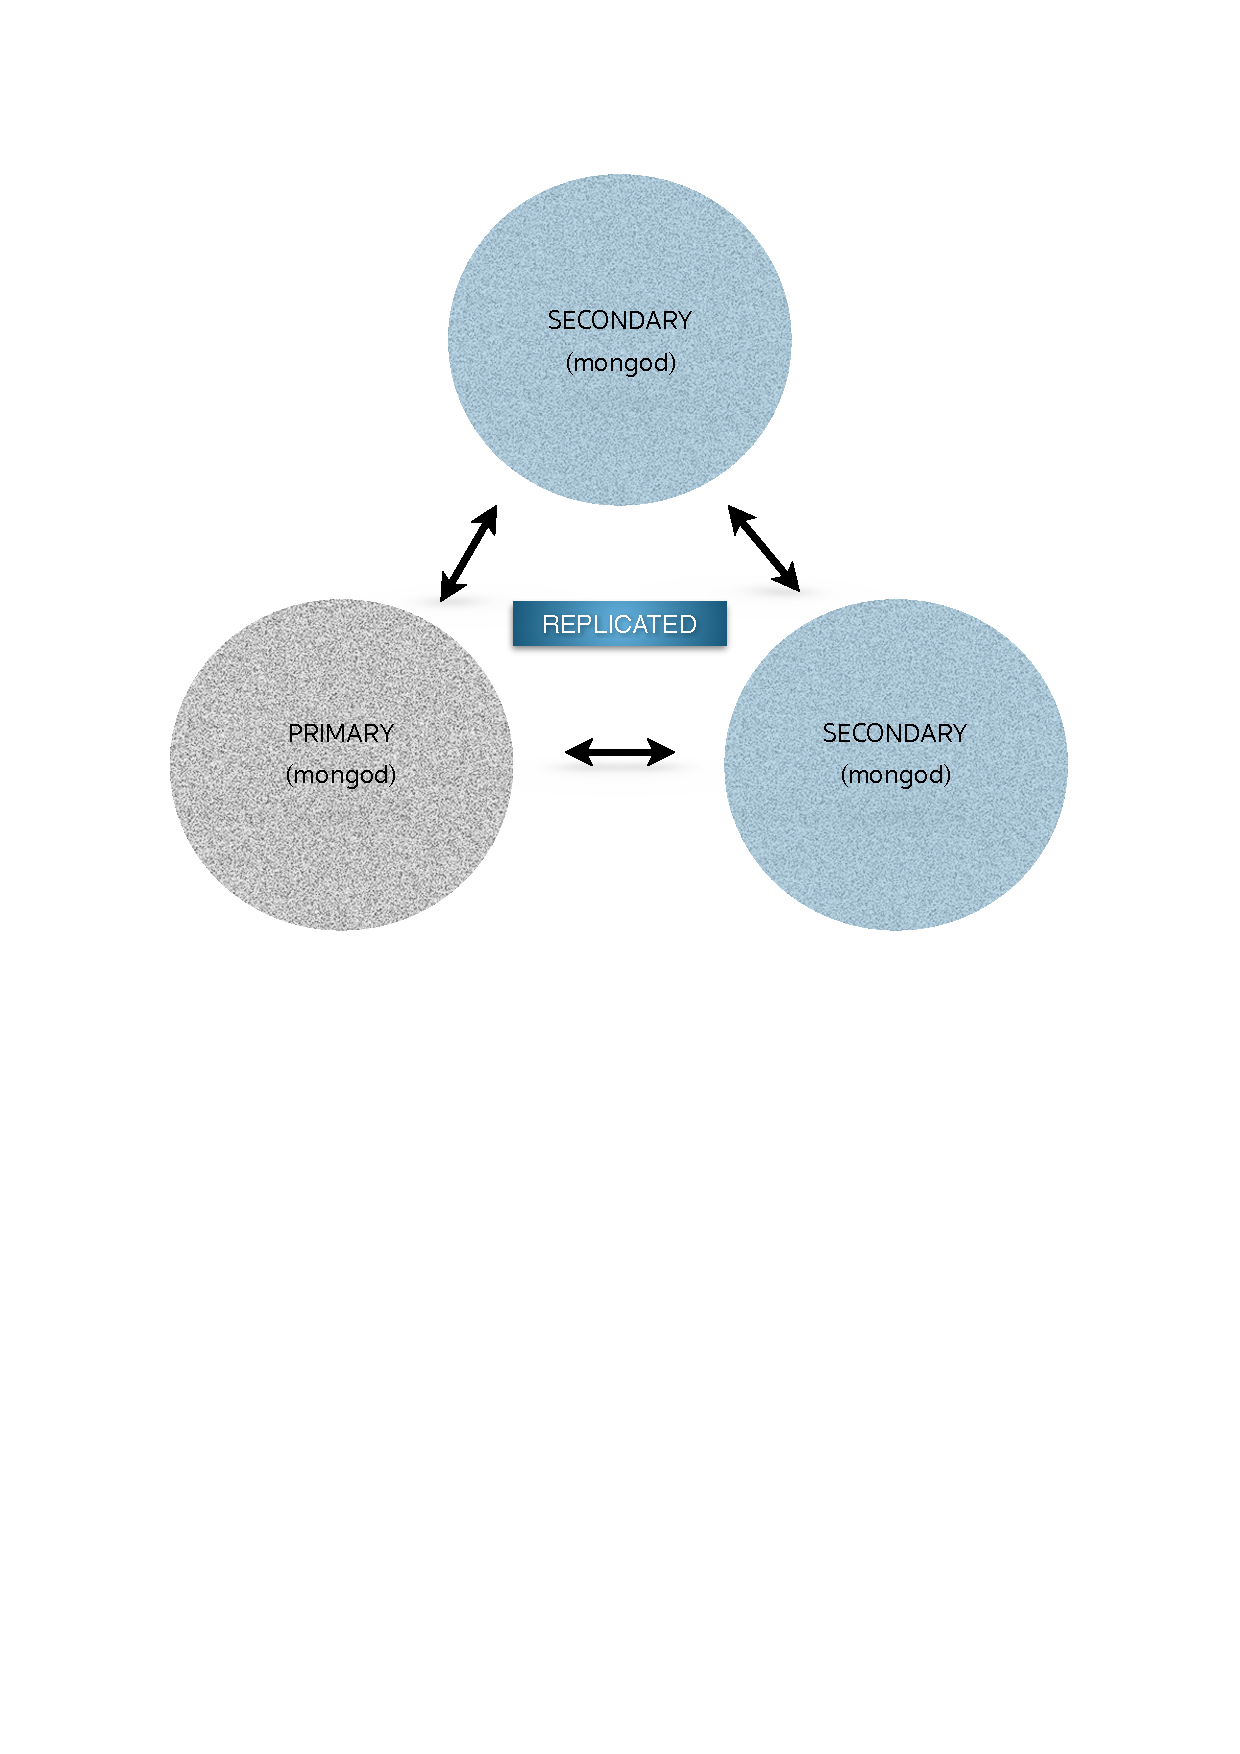
\includegraphics[trim = 0mm 139mm 0mm 28mm, clip, width=0.7\textwidth]{resources/replicaSet/newReplicaSet}
%\caption[Mitglieder der Replikationsgruppe wählten einen neuen \textbf{Primary} aus]{Mitglieder der Replikationsgruppe wählten einen neuen \textbf{Primary} aus}
%\label{img:newReplicaSet}
%\end{figure}



%\paragraph{Eine Replikationsgruppe erzeugen}
%In diesem Teilabschnitt wird eine Replikationsgruppe mit insgesamt drei Servern erzeugt. Jeder Schritt der Konfiguration wird in diesem Teilabschnitt nachgespielt.



%
%Über die sog. \textit{Mongo Shell} auf der Kommandozeile ist es möglich,  zum Serverprozess zu verbinden und nötige Schreib- und Lesezugriffe durchzuführen.
%
%Um eine Replikationsgruppe effizienter erzeugen zu können, wird ein Skript geschrieben. In dem Skript aus der Abbildung \ref{lst:scriptForCreateOfRep} werden erstmals die Ordner zum Speichern der Daten angelegt. Demnächst ....
%
%\begin{listingsboxShell}[label={lst:scriptForCreateOfRep}]{myshell}{Skript fürs Erstellen einer Replikationsgruppe}
%#!/usr/bin/env bash
%
%mkdir -p /data/rs1 /data/rs2 /data/rs3
%
%// Start von drei lokalen mongod-Instanzen als Replikationsgruppe
%
%mongod --replSet m101 --logpath "1.log" --dbpath /data/rs1 --port 27017
%--oplogSize 64 --fork --smallfiles
%mongod --replSet m101 --logpath "2.log" --dbpath /data/rs2 --port 27018
%--oplogSize 64 --smallfiles --fork
%mongod --replSet m101 --logpath "3.log" --dbpath /data/rs3 --port 27019
%--oplogSize 64 --smallfiles --fork
%\end{listingsboxShell}
%
%Das Skript mit dem Inhalt aus Listing \ref{lst:scriptForCreateOfRep} ist mit dem aus Listing \ref{lst:runOfscriptForCreateOfRep} auszuführen:
%
%\begin{listingsboxShell}[label={lst:runOfscriptForCreateOfRep}]{myshell}{Erstellen einer Replikationsgruppe anhand eines Skriptes}
%vlfa:scripts vlfa$ bash < create_replica_set.sh
%\end{listingsboxShell}
%
%Bei der Ausführung des Skriptes kann zu den Problemen führen. Um aktuelle Prozesse mit mongo anschauen und stoppen zu können, muss man folgenden Befehl angeben. The problem was that I have runned mongod without any parameters before I started launching the nodes. First kill all the mongo, mongod and mongos instances to guarantee the environment is clear.\url{http://stackoverflow.com/questions/25839559/mongodb-server-is-not-running-with-replset}
%
%Find the mongodb process PID by typing: lsof -i:27017 assuming your mongodb is running on port 27017
%Type kill <PID>, replace <PID> by the value you found the previous command.
%
%\begin{listingsboxShell}[label={lst:listOfPIDs}]{myshell}{Auflistung aktueller mongo(s,d)-Prozesse}
%vlfa:scripts vlfa$ ps -ef | grep 'mongo'
%
%oder besser mit 
%
%lsof -i:27017
%\end{listingsboxShell}
%
%Danach ist wichtig, Prozesse zu stoppen. Dafür muss man nach dem Befehl kill die ProzessID eingeben, siehe Listing \ref{lst:killPID}. Dann wird die Möglichkeit fürs Erstellen eigener Replikationsgruppe ermöglicht, siehe dazu Listings \ref{lst:scriptForCreateOfRep} und \ref{lst:runOfscriptForCreateOfRep}.
%
%\begin{listingsboxShell}[label={lst:killPID}]{myshell}{mongo(s,d)-Server zwingend stoppen}
%// konkreten mongo(s,d)-Server zwingend stoppen
%vlfa:scripts vlfa$ kill 'PID'
%
%// alle mongo(s,d)-Server zwingend stoppen
%vlfa:scripts vlfa$ killall mongo(s,d)
%\end{listingsboxShell}
%
%Damit ist die Konfigurationsgruppe mit 3 Servern angelegt. Zum Anschauen einer log-Datei;
%
%\begin{listingsboxShell}[label={lst:X}]{myshell}{1.log-Inhalt}
%2016-12-19T14:58:11.637+0100 I CONTROL  [initandlisten] MongoDB starting :
%pid=25626 port=27017 dbpath=/data/rs1 64-bit host=vlfa.fritz.box
%// irrelevant
%2016-12-19T14:58:11.639+0100 I CONTROL  [initandlisten] options:
%{ net: { port: 27017 }, processManagement: { fork: true }, replication:
%{ oplogSizeMB: 64, replSet: "m101" }, storage: { dbPath: "/data/rs1",
%mmapv1: {smallFiles: true}}, systemLog: {destination: "file", path: "1.log"}}
%// irrelevant
%\end{listingsboxShell}
%Die Replikationsgruppe starten.......blabla
%\begin{listingsboxJavaScript}[label={lst:initReplica}]{myJS}{Skript zum Start der Replikationsgruppe}
%config = { _id: "m101", members:[
%          { _id : 0, host : "localhost:27017", priority:0, slaveDelay:5},
%          { _id : 1, host : "localhost:27018"},
%          { _id : 2, host : "localhost:27019"} ]
%};
%
%rs.initiate(config);
%rs.status();
%\end{listingsboxJavaScript}
%
%Die Server aus Listing \ref{lst:initReplica} nehmen nun Kontakt miteinander auf, gründen die Gruppe und wählen den Primary-Server aus. Wie im Skript aus Listing 	\ref{lst:initReplica} zu entnehmen ist, kann der Zustand der Replikationsgruppe mit \texttt{rs.status()} geprüft werden. Bei Ausfall des Primary-Servers wählen die Secondaries untereinander entsprechend einen neuen Primary-Server. Damit wird die Ausfallsicherheit des Servers erreicht. Die Mindestanzahl an Server in einer Replikationsgruppe liegt bei drei. 
%
%\begin{listingsboxShell}[label={lst:runOfInitReplica}]{myshell}{Skript ausführen}
%vlfa:scripts vlfa$ mongo --port 27018 < init_replica.js
%\end{listingsboxShell}
%
%Die Priorität '0' teilt mit, wer Primary Member in der Replikationsgruppe ist. Korrigieren, Stimmt nicht....\url{https://docs.mongodb.com/v3.2/core/replica-set-priority-0-member/}


%\paragraph{\colorbox{yellow}{GridFS}}
\paragraph{GridFS}
Für die Daten, die eine Größe in Höhe von 16MB überschreiten, stellt \mongo\ ein Dateisystem namens \textbf{GridFS} zur Verfügung. Abgelegt werden solche Daten in zwei spezielle \textit{Collections}:

\begin{itemize}

\item \textit{fs.files} - die \textit{fs.files-Collection} enthält die Metainformationen zu den einzelnen Dokumenten. Listing \ref{lst:fsFileDocument} veranschaulicht ein Beispiel dazu.
\item \textit{fs.chunks} - in \textit{fs.chunks-Collection} werden die eigentlichen Daten gespeichert.

\end{itemize}

\begin{listingsboxJava}[label={lst:fsFileDocument}]{myjson}{Beispiel für ein Dokument in \textit{fs.files-Collection}}
{
	"_id" : ObjectId("58f5f0056ce5d24528e152c3"),
	"filename" : "Bicycle.jpeg",
	"aliases" : null,
	"chunkSize" : NumberLong(261120),
	"uploadDate" : ISODate("2017-04-18T10:52:53.974Z"),
	"length" : NumberLong(68090),
	"contentType" : "image/jpeg",
	"md5" : "85a866edfca999c0163e7bbc7cd5269b"
}
\end{listingsboxJava}

%\paragraph{\colorbox{yellow}{Treiber für MongoDB}}
\paragraph{Treiber für MongoDB}
Alle mögliche Operationen, die \mongo\ zur Verfügung stellt, sind nicht nur auf \textit{Shell-}Ebene, sondern auch in vielen gängigen Programmiersprachen, wie zum Beispiel Java, C++, C\#, PHP, Python etc. durch bereitgestellte \mongo's Treiber\footnote{MongoDB Drivers: \url{https://docs.mongodb.com/ecosystem/drivers/}, zugegriffen am 18. Februar 2017} möglich.

\subsubsection{Apache Cassandra}
%\subsubsection{\colorbox{yellow}{Apache Cassandra}}

In diesem Kapitel wird ein weiterer wichtiger Vertreter der NoSQL-Datenbanken vorgestellt, nämlich \cass.

\cass\ war ursprünglich eine proprietäre Datenbank von Facebook und wurde 2008 als Open-Source-Datenbank veröffentlicht. Konzipiert ist \cass\ als skalierbares, ausfallsicheres System für den Umgang mit großen Datenmengen auf verteilten Systemen (Clustern) und im Gegensatz zu \mongo\ (C++) in Java geschrieben.

%Zunächst werden die Konzepte von \cass\ allgemein diskutiert und dann die Unterschiede zu der schon besprochenen NoSQL-Datenbank \mongo\ gezeigt.

%Die spaltenorientierten Datenbanken können Datensätze mit beliebiger Spaltenanzahl aufnehmen. Je Datensatz kann über bis zu 2 Milliarden Spalten verfügen.
Im Vergleich zu der \mongo-Datenbank, die in Replikation nach dem Master-Slave-Prinzip funktioniert, verfolgt \cass\ komplett anderes Prinzip. %Dieses Prinzip wird in der Architektur der \cass\ erläutert.

\paragraph{Architektur}
%\paragraph{\colorbox{yellow}{Architektur}}

\begin{itemize}
\item \cass\ ist nach peer-to-peer\footnote{Peer-to-Peer-Netze (P2P) sind Netze, bei denen alle Knoten im Netz dezentral sind.} verteiltes System aufgebaut. Ein peer-to-peer verteiltes System beschreibt ein Cluster, bestehend aus mehreren gleichberechtigten Knoten.  
\item Jeder Knoten ist in so einem Cluster dezentral, unabhängig und akzeptiert sowohl Schreib- als auch Leseoperationen.
\item Falls irgendeiner Knoten aus dem definierten Cluster ausfällt, werden die Schreib- und Leseanforderungen von anderen verfügbaren Knoten bedient.
\end{itemize}
\cass\ stellt die Verfügbarkeit und Partitionstoleranz über die Konsistenz.

\paragraph{Datenmodell}
%\paragraph{\colorbox{yellow}{Datenmodell}}

Die Hauptbestandteile des Datenmodells von \cass\ veranschaulicht die Abbildung \ref{img:cassandraDataModel}.
\begin{itemize}
\item Cluster
\item Keyspace
\item Column Family
\item Row
\item Column sowie
\item Value
\end{itemize}
\begin{figure}[H]
\centering
%trim = links, unten, rechts, oben
 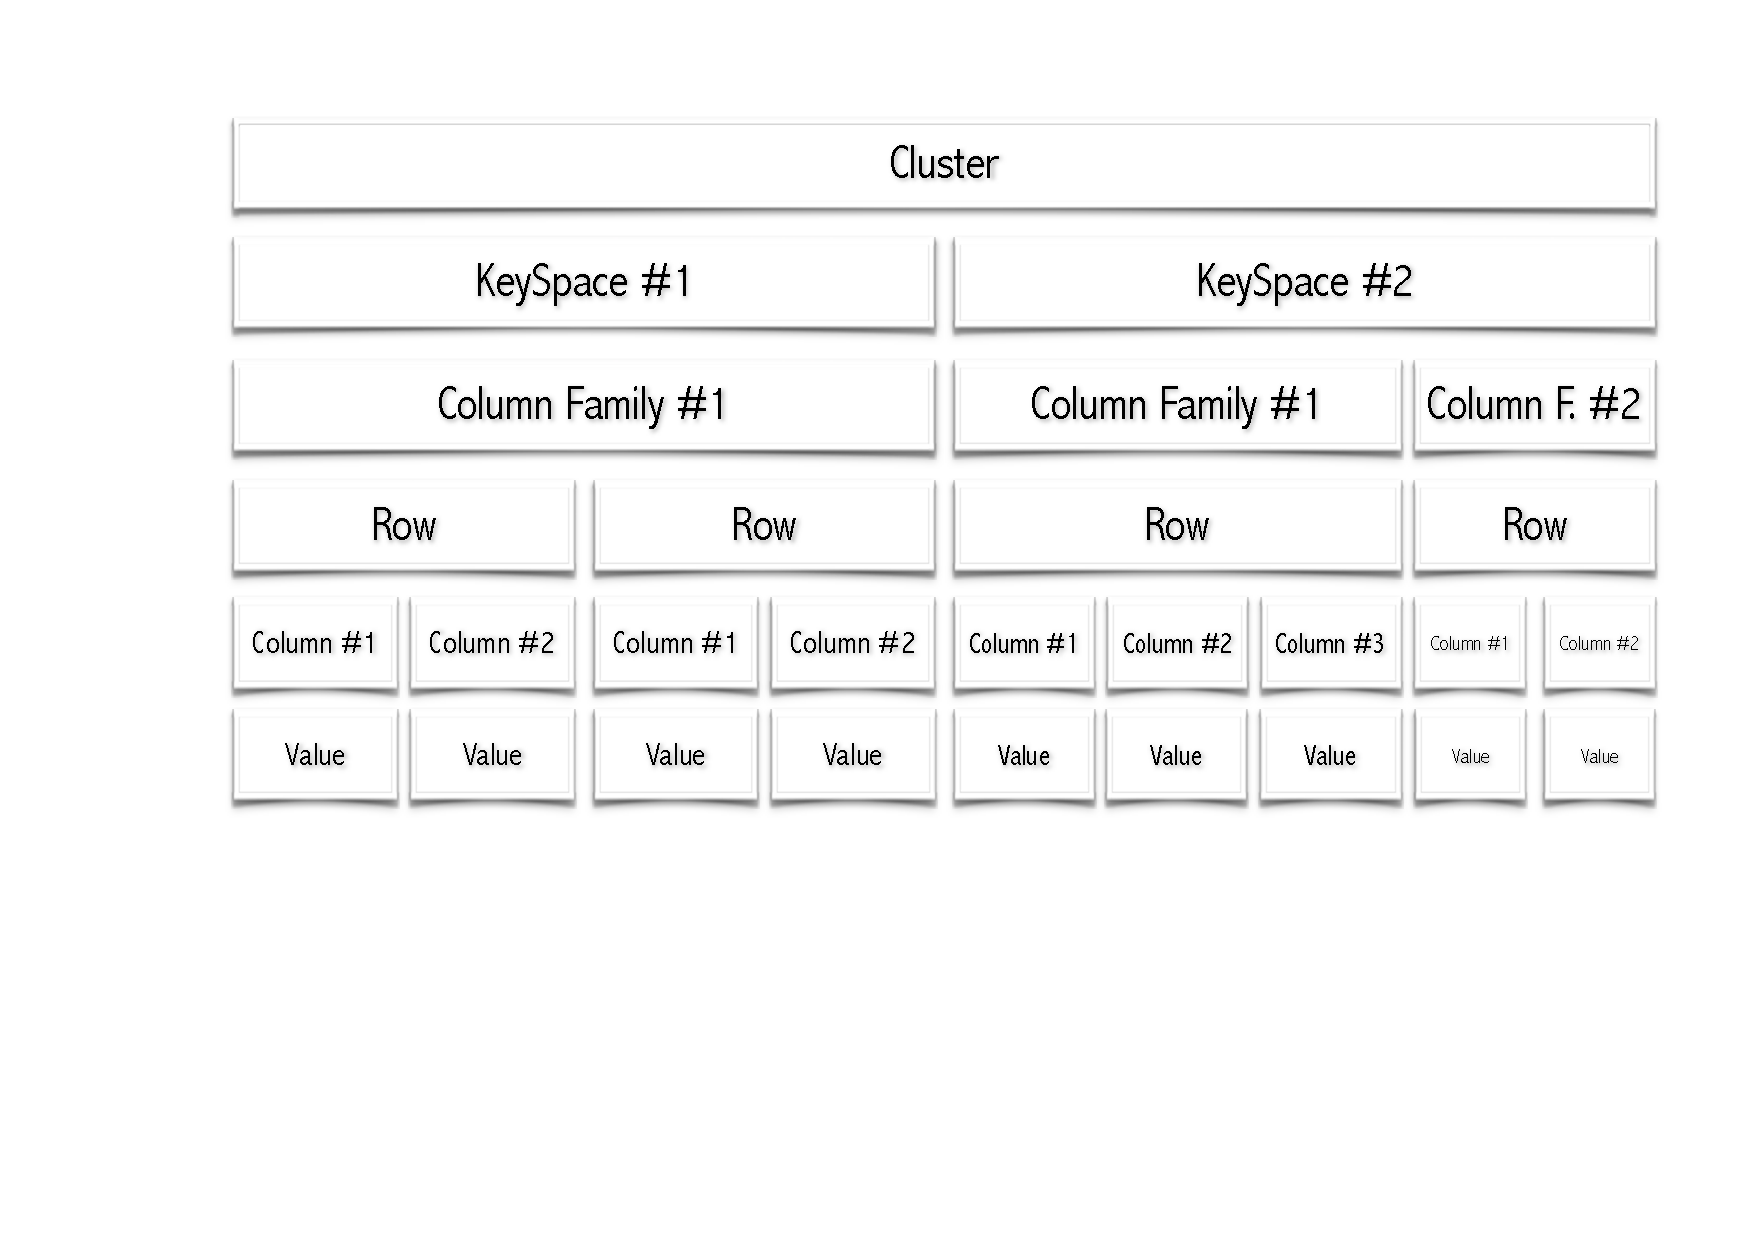
\includegraphics[trim = 25mm 70mm 15mm 15mm, clip, width=0.9\textwidth]{resources/cassandra/cassandraDataModel}
\caption[Datenmodell]{Datenmodell}
\label{img:cassandraDataModel}
\end{figure}
\cass\ definiert einen Datenbankserver als ein Cluster, auf dem mehrere Datenbanken (Keyspaces) angelegt werden. Eine Spaltenfamilie (Column Family) entspricht einer Tabelle und enthält Zeilen (Rows), welche mit einer eindeutigen \textit{Id} zu identifizieren sind. In Zeilen (Rows) werden die Datensätze gespeichert, wobei jede Zeile bis zu 2 Milliarden Spalten (Columns) enthalten kann. Die Spalten (Columns) dagegen enthalten jeweils ein Paar „Schlüssel-Wert“ (Key-Value-Paar). 
Um bei Leseoperationen einen effizienteren Zugriff erreichen zu können, müssen die Spalten (Columns) Super Columns definieren, indem mehrere Spalten zusammengesetzt werden.

\subsection{Spring Framework}
%\subsection{\colorbox{yellow}{Spring Framework}}

Das Spring Framework ist ein Open Source Java Framework, welches einfache Java Objekte, sogenannte Plain-Old-Java-Objects (POJO), als \textbf{Spring-Beans} verwaltet. Dabei stellt das Spring Framework unter Anderem einen \textit{Inversion of Control Container} zu Verfügung, der per \textit{Dependency Injection} abhängige Spring-Beans miteinander verknüpft und konfiguriert.

Die wesentlichen Funktionen des Spring Frameworks sind:
\begin{itemize}
	\item Plain-Old-Java-Objects basierendes Programmiermodell.
	\item Verknüpfungen durch DI über den \textit{Inversion-of-Control Container}.
\end{itemize}

%\subsubsection{\colorbox{yellow}{Module des Spring Frameworks}}
\subsubsection{Module des Spring Frameworks}

Spring Framework besteht aus Modulen, die den Entwicklern unabhängig zur Verfügung stehen. Die folgenden drei Module werden für die Umsetzung der Architektur vorgeschlagen.

\begin{itemize}
	\item Spring Core Container - Das Basismodul, das den \textit{Inversion of Control Container} und die Funktionen für die \textit{Dependency Injection} bereitstellt. Die Anwendungsobjekte existieren in einer Spring-basierten Anwendung in einem Spring Core Container \textbf{(Abb. \ref{img:container})}. Der Spring Core Container erstellt Objekte, verschaltet und konfiguriert sie. Weiterhin übernimmt der Spring Core Container die Kontrolle über den Lebenszyklus der Objekte. In der Spring Terminolgie heißen die von einem Spring-Container verwalteten Objekte \textbf{Spring-Beans} oder einfach \textbf{Beans}.

\begin{figure}[H]
\centering
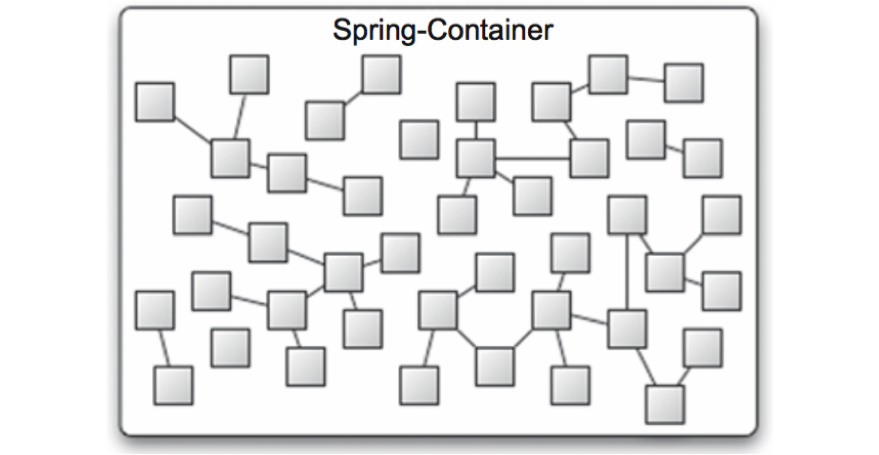
\includegraphics[width=3.0in]{resources/container}
\caption[Spring Core Container für Beans]{Spring Core Container für Beans}
\label{img:container}
\end{figure}

Seit Erscheinen der Springs-Version 1.0 im Jahr 2004 müsste man den Container mit XML konfigurieren. Ausgehend von Springs-Version 2.5 im Jahr 2007 wurde der Aufwand der XML-Konfiguration in einer Spring-basierten Anwendung durch die Kombination mit @-Annotationen extrem reduziert. Mit der Springs-Version 3.0 ist es endlich möglich geworden, den Spring-Container vollständig ohne XML-Konfiguration zu erzeugen. Diese Konfiguration ohne XML-Konfiguration nennt man \textbf{Java-basierte Konfiguration}.

	\item Spring Web - Das MVC-Framework mit der Möglichkeit REST-Webanwendungen umsetzen zu können. Dazu wird das MVC-Pattern implementiert. Zusätzlich werden allgemeine Web-Technologien wie HTTP zu Verfügung gestellt.
	\item Spring Boot - Mit diesem Module können Self-Contained Anwendungen erstellt werden. Diese Art von Anwendungen werden in einem einzelnen JAR/WAR ausgeliefert, abhängig von Konfiguration. Zusätzlich werden die Abhängigkeiten aller benötigten Bibliotheken durch Spring Boot verwaltet.\footnote{Das Spring Framework, \url{https://www.frank-rahn.de/einfuehrung-spring-framework/\#toggle-id-1}, zugegriffen am 18. Februar 2017}
	\end{itemize}

\subsubsection{Konfiguration mit Maven}
%\subsubsection{\colorbox{yellow}{Konfiguration mit Maven}}

Um Spring Framework in einer Java Anwendung verwenden zu können, müssen die entsprechenden Bibliotheken dem Java Projekt hinzugefügt werden. Listing \ref{lst:pom} zeigt ein Beispiel für eine Maven\footnote{Maven, \url{https://maven.apache.org}, zugegriffen am 20. Februar 2017}-Konfigurationsdatei, in der benötigte Bibliotheken für Spring deklariert sind.

\begin{listingsboxJava}[label={lst:pom}]{myxml}{Konfiguration mit \texttt{pom.xml}}
	<!-- Spring Core Container Modul -->
	<dependency>
		<groupId>org.springframework</groupId>
		<artifactId>spring-core</artifactId>
	</dependency>

	<!-- Spring Web Modul -->
	<dependency>
		<groupId>org.springframework</groupId>
		<artifactId>spring-web</artifactId>
	</dependency>
	
	<!-- Spring Boot Starter Modul -->
	<dependency>
		<groupId>org.springframework.boot</groupId>
		<artifactId>spring-boot-starter-web</artifactId>
	</dependency>
\end{listingsboxJava}
Maven wird verwendet, um die Abhängigkeiten zu den externen Bibliotheken zu verwalten. Die benötigten Bibliotheken werden von User in der Maven- Konfigurationsdatei \texttt{pom.xml} als Abhängigkeiten (engl. \texttt{dependencies}) deklariert und das Tool lädt die Bibliotheken automatisch herunter, speichert die in einem lokalen Repository und fügt sie dann dem Projekt hinzu.

\subsection{\colorbox{red}{Rest Server}}
DER KOMMT DOCH MIT SPRINGGGGGGGG

\subsection{\colorbox{red}{AngularJS 2 - JavaScript Framework}}
%\subsection{AngularJS 2 - JavaScript Framework}

Angular 2 ist ein JavaScript Framework, das für Frontend-Teil der Webanwendungen verwendet wird, um Single-Page-Webanwendungen modern aufbauen zu können. Bezüglich Wartbarkeit von Single-Page-Webanwendungen sind in JavaScript-Welt folgende Konzepte wie Komponentenorientierung und Dependency Injection durch Angular 2 möglich geworden.

Angular 2 ist komplett in TypeScript entwickelt worden. TypeScript ist eine JavaScript-Erweiterung von Microsoft, die JavaScript um optionale statische Typprüfung und objektorientierten Programmierstil über die Nutzung von Interfaces, Klassen, Module etc. erweitert\footnote{AngularJS und TypeScript, \url{https://jaxenter.de/angularjs-und-typescript-der-beginn-einer-wunderbaren-freundschaft-17957}, zugegriffen am 26.Februar 2017}.

 \clearpage
%\chapter{Architektur}
\chapter{\colorbox{yellow}{Architektur}}

\section{Einführung}

Die typische \textbf{MVC}-basierte Architektur einer Webanwendung ist in der Abbildung \ref{img:architectureMyApp} abgebildet.

%\begin{wrapfigure}{r}{0.37\textwidth}
%\begin{center}
%\vspace{-35pt}%
%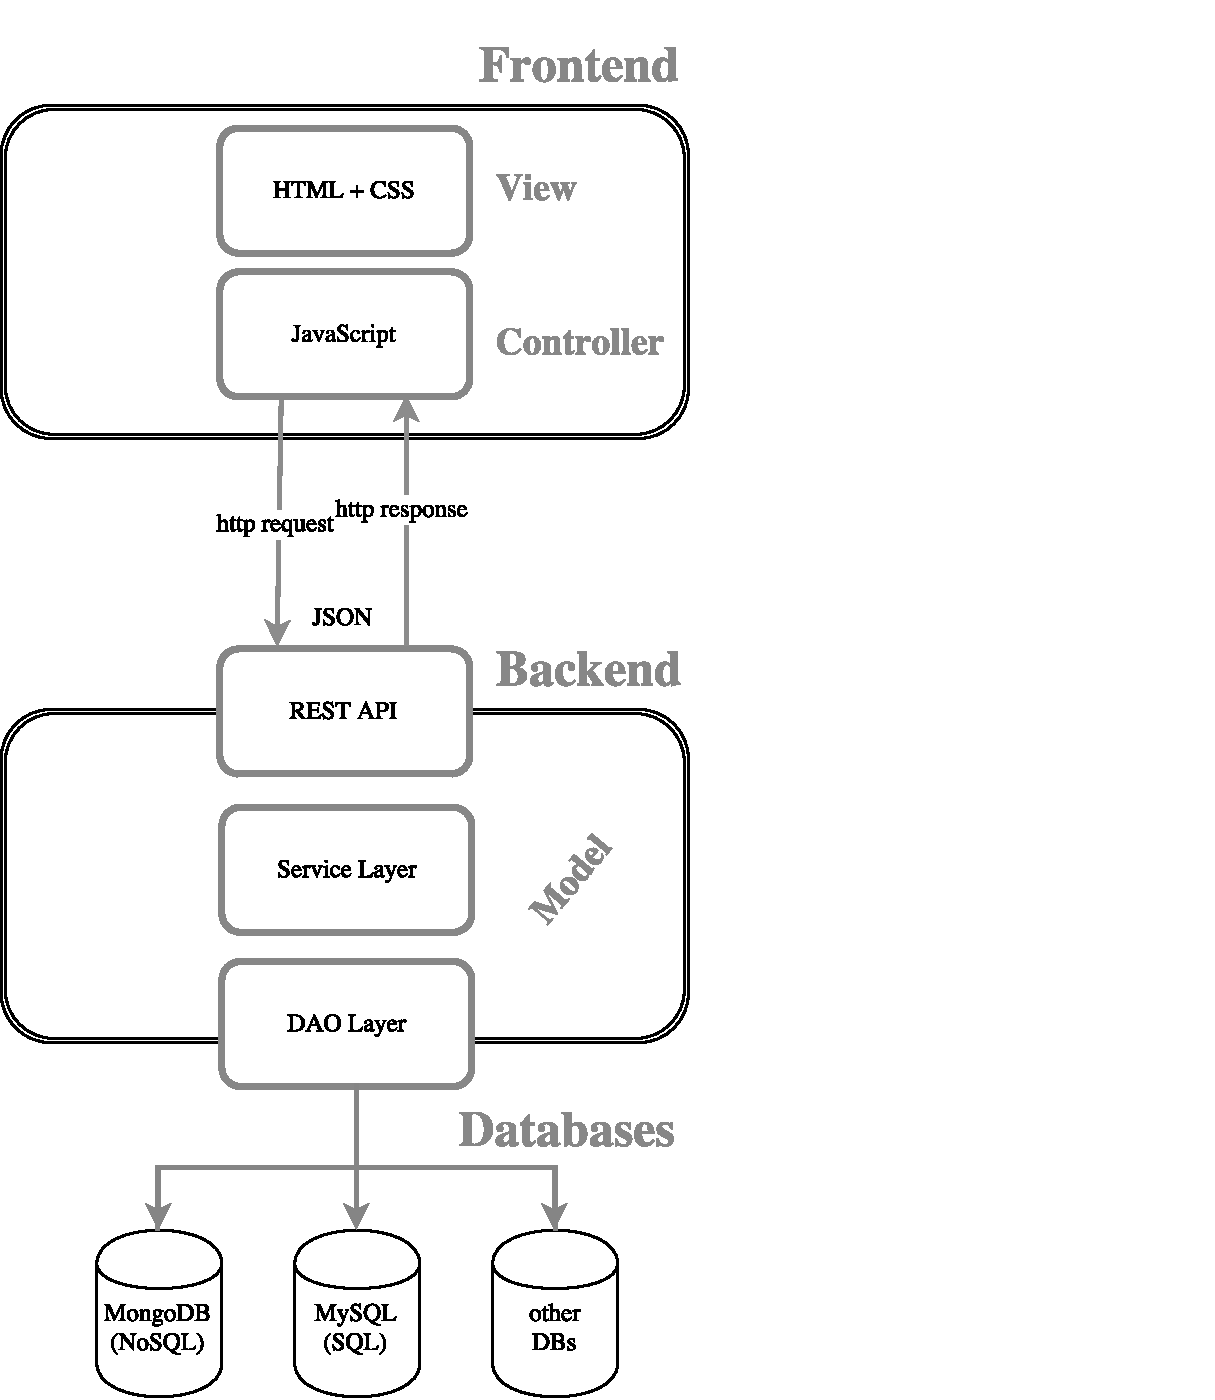
\includegraphics[trim = 0mm 0mm 0mm 0mm, clip, width=0.3\textwidth]{resources/architectureMyAppWithoutFrameworks}
%\caption[Architektur-Prototyp]{Architektur-Prototyp}
%\label{img:architectureMyApp}
%\vspace{-35pt}%
%\end{center}
%\end{wrapfigure}

\begin{figure}[H]
\vspace{-20pt}%
\centering
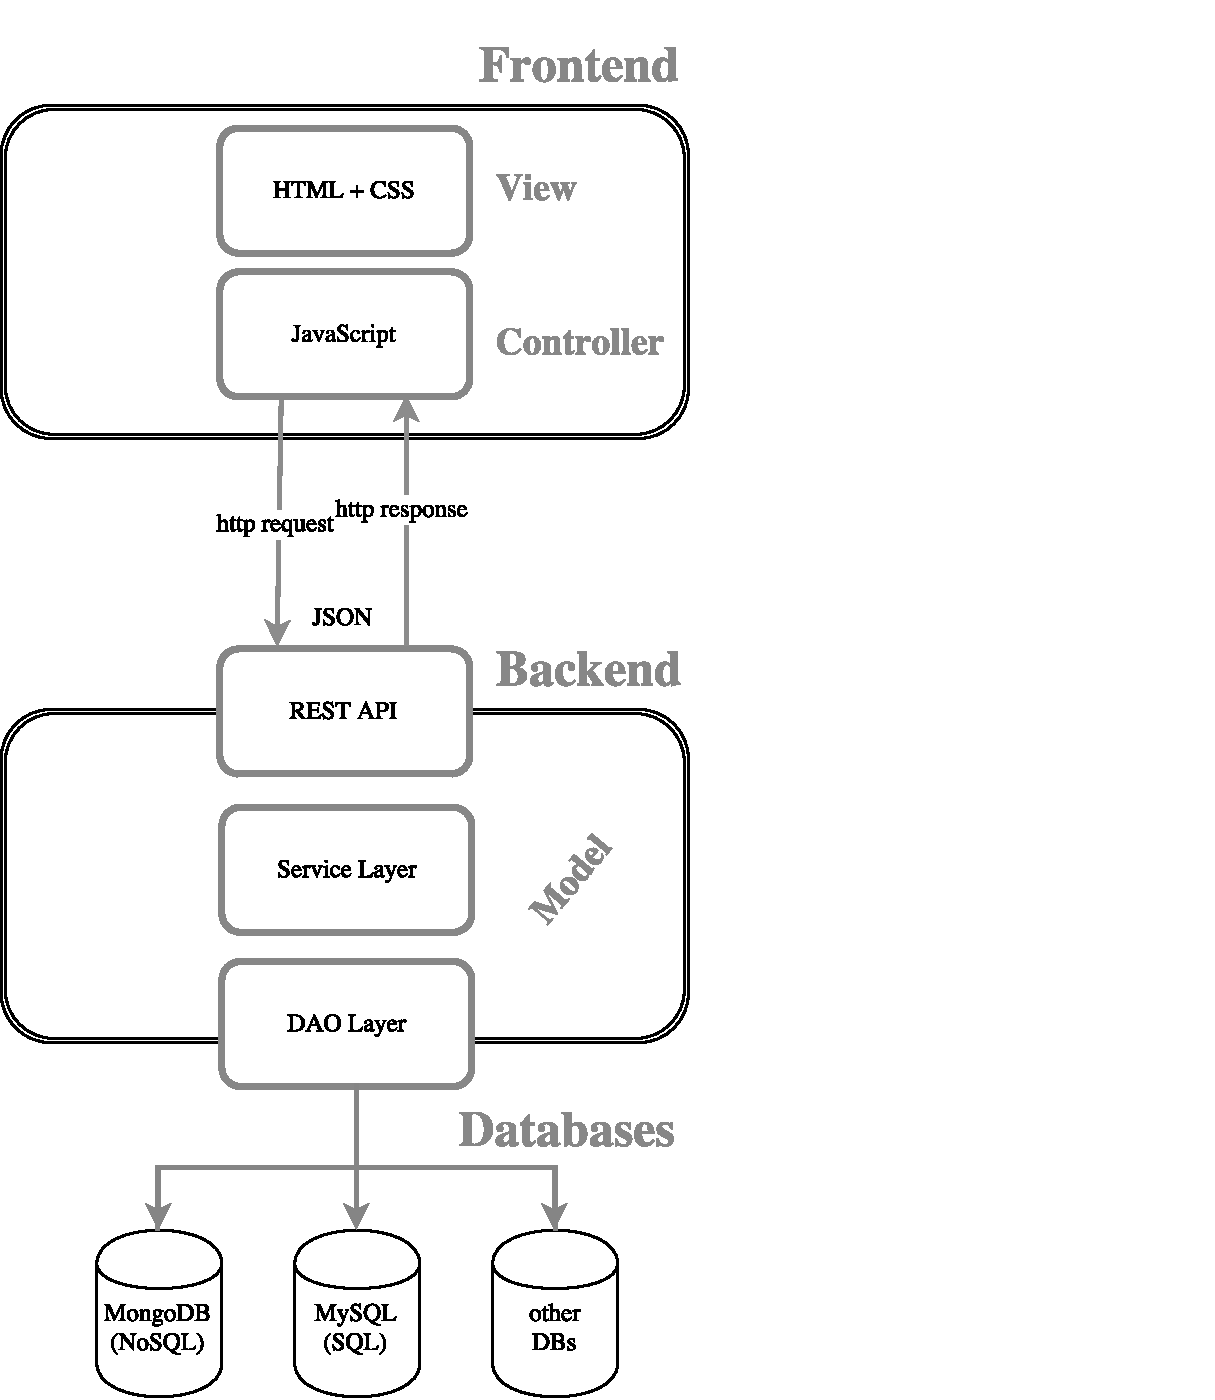
\includegraphics[trim = 0mm 0mm 0mm 0mm, clip, width=0.35\textwidth]{resources/architectureMyAppWithoutFrameworks}
\caption[Architektur-Prototyp]{Architektur-Prototyp}
\label{img:architectureMyApp}
\end{figure}

Der Web-Client, bestehend aus View und Controller wird auf dem Rechner des Anwenders ausgeführt, z. B. in der Browser-Anwendung. Es gibt einen Server (Backend) mit dem der Web-Client kommuniziert, um die Daten abzufragen oder zu ändern. Der Backend-Teil nutzt eine Datenbank, um die Daten persistent zu speichern. Es wird angenommen, dass die Webapplikation für eine große Anzahl von Internetnutzern ausgelegt ist. Das Ziel ist, dass unabhängig von der Anzahl der Nutzer, die die Webanwendung gleichzeitig nutzen wollen, die Webanwendung die konstante Antwortzeiten hat. In dieser Architektur gibt es zwei Komponenten, die bei der steigenden Anzahl von Usern die Antwort verlangsamen können:

\begin{itemize}

\item der Backend-Server, der eine begrenzte Anzahl von \textbf{HTTP}\footnote{\textbf{HTTP} ist ein zustandloses Protokoll zur Übertragung der Daten zwischen Web-Client (=Browser Anwendung) und Web-Server. Jede neue Anfrage, die vom Web-Client erfolgt, erfordert einen neuen Verbindungsaufbau und erneute Datenbeschaffung.}-Anfragen bearbeiten kann. Es ist auch denkbar, dass der Backend-Server auch Geschäftslogik implementiert und auch dafür die  Ressourcen zusätzlich aufwenden muss und

\item die Datenbank. Die Datenbank kann nur eine bestimmte Anzahl der Abfragen gleichzeitig beantworten.

\end{itemize}

Demzufolge, um die konstante Antwortzeiten der Webanwendung bei der steigenden Anzahl von Usern beizubehalten, ist eine Skalierungsstrategie für diese beide Komponente notwendig. Es reicht nicht nur eine zu skalieren, weil dann letztendlich die andere Komponente zum Flaschenhals wird.

Es wird für eine horizontale Skalierung für beide Komponenten entschieden, weil die vertikale Skalierung ihre Grenzen hat.

\section{Konzept}

\textit{Load Balancer}\footnote{Load Balancer, \url{https://f5.com/glossary/load-balancer}, zugegriffen am 21.02.2017} gilt als ein Verteiler, der die Web-Client Anfragen entgegennimmt und sie an mehrere parallel laufende Server verteilt, je nach Maschinenüberlastung. Dabei berücksichtigt \textit{Load Balancer}, dass die Last an Servern gleichmäßig verteilt wird, um die Anwendungs-Performance zu verbessern.
%\begin{wrapfigure}{l}{0.42\textwidth}
%\begin{center}
%\vspace{-20pt}%
%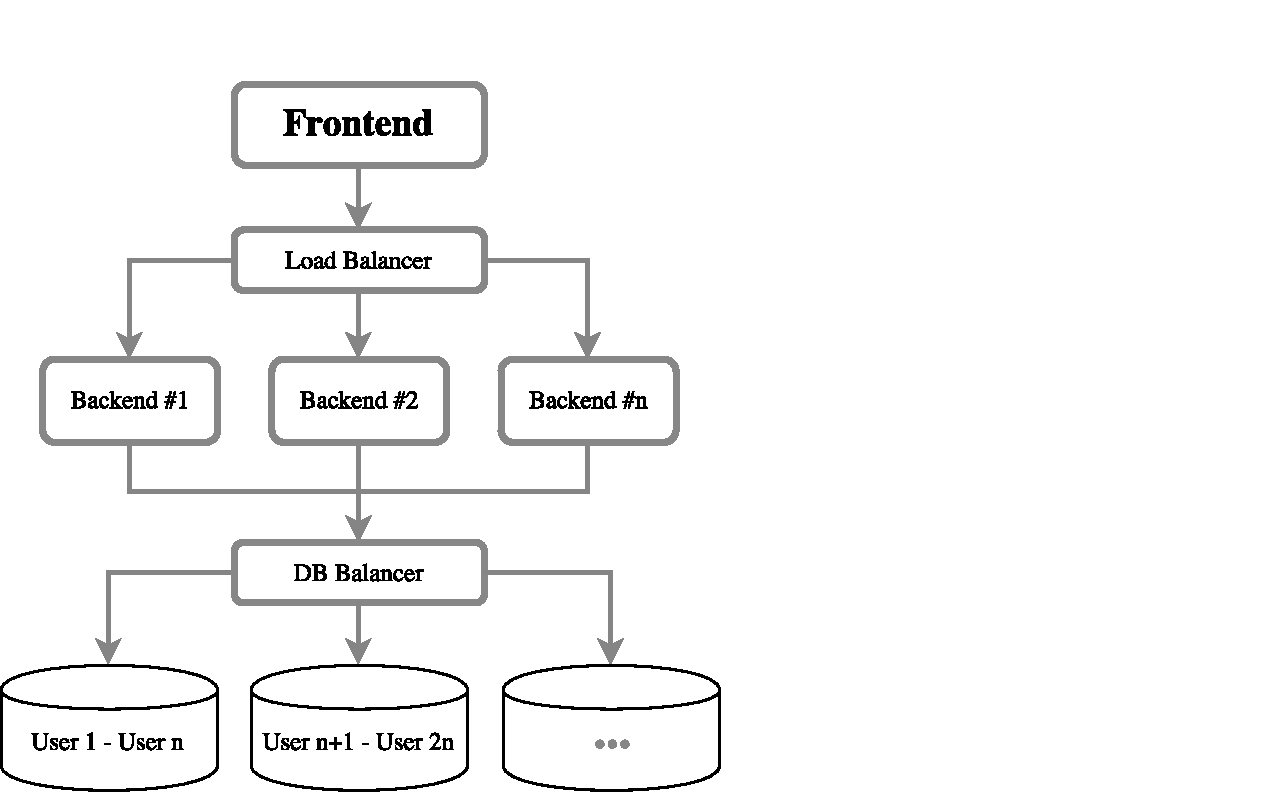
\includegraphics[trim = 0mm 0mm 0mm 0mm, clip, width=0.4\textwidth]{resources/ueberblickArchitektur}
%\caption[Überblick zur vorgeschlagenen Architektur]{Überblick zur vorgeschlagenen Architektur}
%\label{img:ueberblickArchitektur}
%\vspace{-30pt}%
%\end{center}
%\end{wrapfigure}

\begin{figure}[H]
%\vspace{-20pt}%
\centering
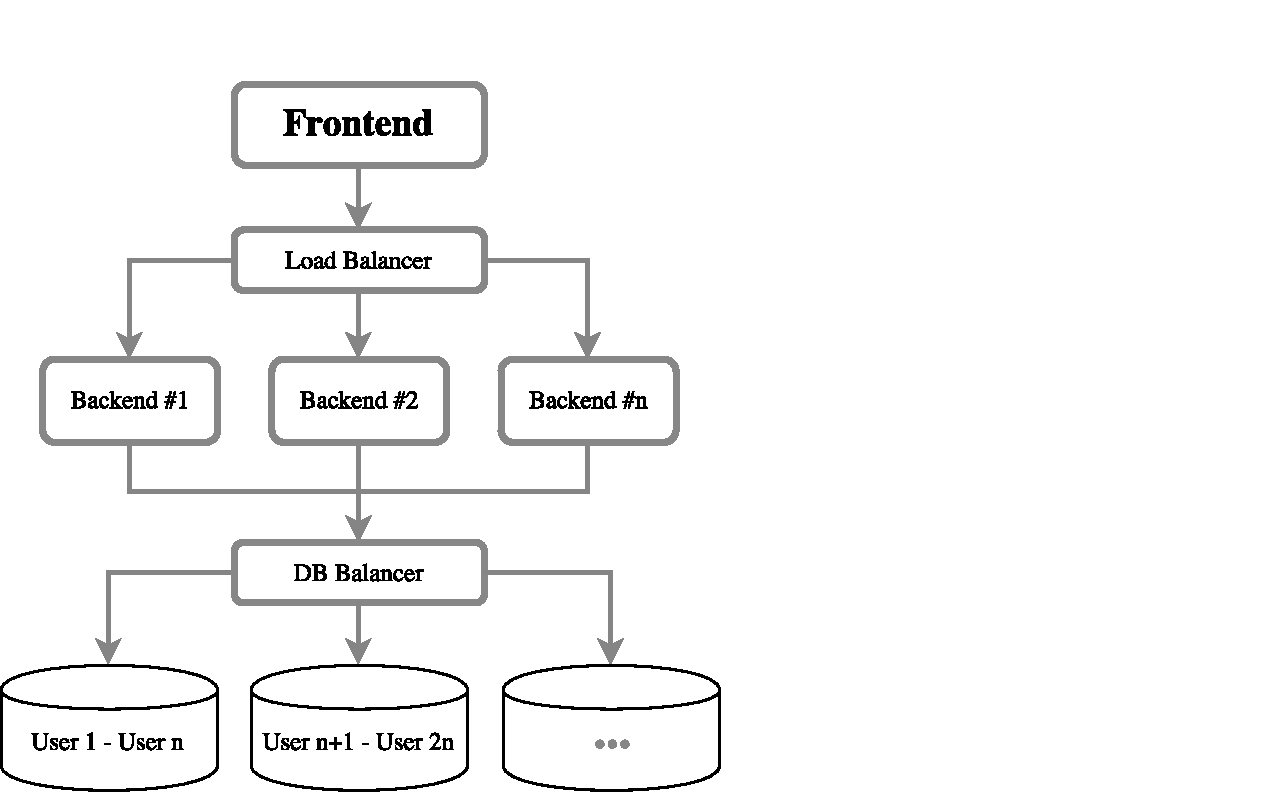
\includegraphics[trim = 0mm 0mm 0mm 0mm, clip, width=0.5\textwidth]{resources/ueberblickArchitektur}
\caption[Überblick zur vorgeschlagenen Architektur]{Überblick zur vorgeschlagenen Architektur}
\label{img:ueberblickArchitektur}
\end{figure}


Der Zugriff auf Funktionen in Backend-Teilen erfolgt über \textit{REpresentational State Transfer} oder kurz \textbf{REST}. Durch die Verwendung von REST erfolgen die Web-Client-Anfragen auf Basis des \textbf{HTTP}-Protokolls. Der Web-Client sendet HTTP-Request und erwartet HTTP-Response, in dem Fall des implementierten Prototyps im \textit{JSON}-Format.

Der Zustand \textit{(=Session)} der Web-Client-Anfragen wird im Frontend-Teil implementiert und der Web-Server enthält keine Information über Session, da dieser \textit{stateless} arbeitet. \textit{Stateless} bedeutet, dass die Web-Clients mit jeder Anfrage einen neuen Verbindungsaufbau und erneute Datenbeschaffung erfordern und diese voneinander unabhängig sind. Gleich nach einer Web-Server Response wird die Verbindung geschlossen und der Zustand bleibt nicht gespeichert. Somit ist bei einer \textit{stateless-}Webanwendung Sessions nicht möglich.

Falls nach dem Anwendungskontext eine Zustandsspeicherung gefordert wird, wäre die Umsetzung in einer \textit{stateful}-Webanwendung möglich. Bei einer \textit{stateful}-Webanwendung werden Web-Client Anfragen zu einer gemeinsamen logischen Sitzung zusammengefasst, um alle Nutzerinteraktionen hinweg in einem einzigen Kontext auszuführen. Dies wird mithilfe von \textit{Session-Cookies}\footnote{Session-Cookie, \url{https://help.sap.com/erp2005_ehp_04/helpdata/de/cc/d6eef928f711d5991f00508b6b8b11/content.htm}, zugegriffen am 20.01.2017} realisiert.

Bei \textit{stateful}-Anwendungen muss der \textit{Load Balancer} so konfiguriert sein, dass alle von einem Web-Client kommenden Requests an einen Server weitergeleitet werden können, was komplexer ist, als bei \textit{stateless}-Anwendungen. 

Die eigentliche horizontale Skalierung der Daten findet auf der Datenbankebene statt. Die Daten werden in die Datenbank ständig geschrieben und gelesen. Um bei diesen Prozessen eine gute Performance auch auf Datenbankebene zu erreichen, wird angeboten, die Daten auf Knoten zu verteilen. Für weitere Requests wird eine Komponente geben, die anhand der Informationen in Requests erkennen wird, wo genau die Daten abgelegt sind. 
%- WriteConcern in MongoDB: abhängig vom Anwendungskontext, ob in dieser mehr write oder mehr read-Operationen durchgeführt werden, muss mongoDB so konfigutiert werden, dass die Anfragen gut skalierbar sind. Es ist möglich, die Read-Operationen bei Secondaries zu aktivieren, dabei muss man aber auch den Ablauf der Transaktion so zu konfigurieren, dass die Transaktion erst dann abgeschlossen ist, wenn die Daten auf allen Knoten repliziert sind, danach wird die Transaktion als abgeschlossen gezählt.

%\begin{wrapfigure}{r}{0.4\textwidth}
%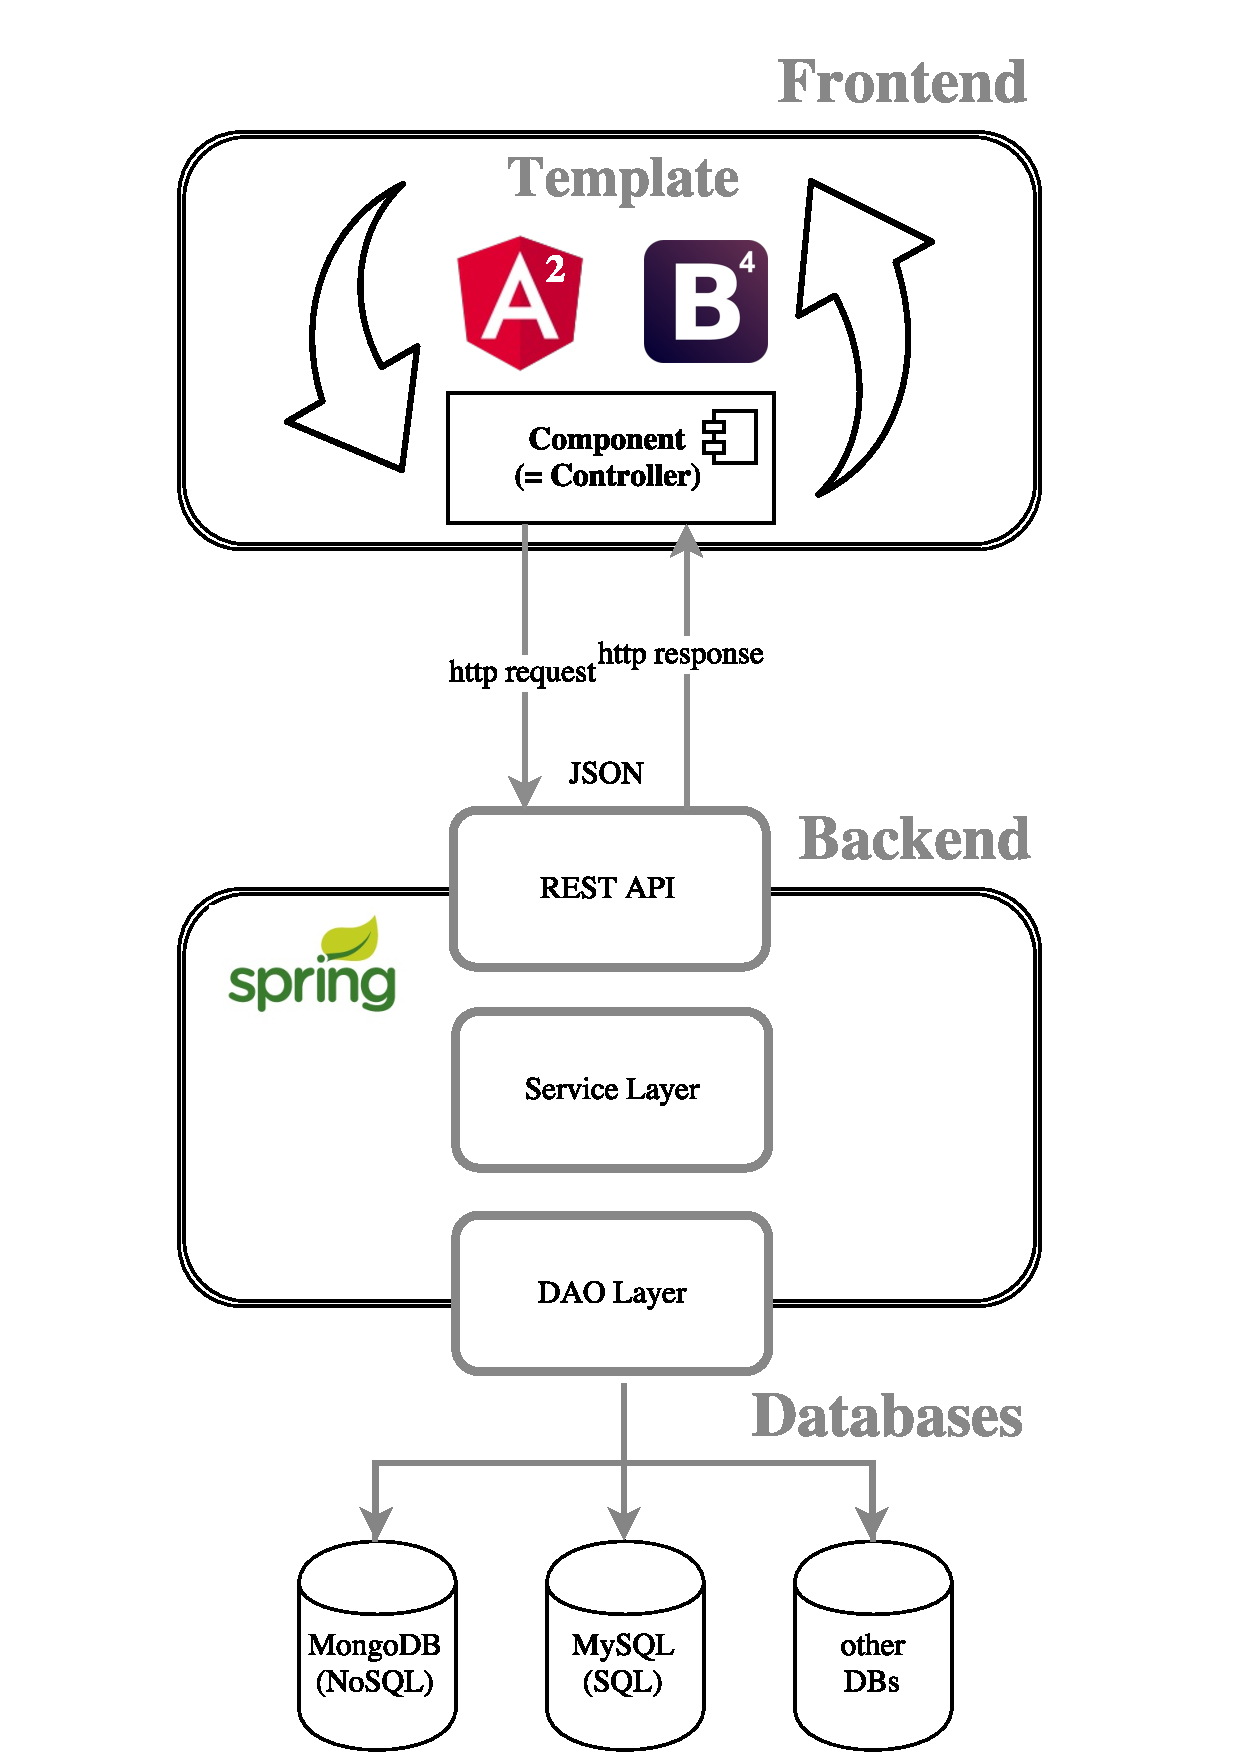
\includegraphics[trim = 20mm 0mm 30mm 9mm, clip, width=0.4\textwidth]{resources/architectureMyApp}
%\caption[Architektur-Prototyp]{\label{img:myArchitecture}Architektur-Prototyp}
%\end{wrapfigure}

%\section{Datenhaltungsschicht (Databases)}
\section{Umsetzung}




 \clearpage
%%\chapter{Zu empfehlende Architektur}
%\chapter{Empfohlene Architektur}
\chapter{Implementierung}\label{implement}

\section{Fachliche Spezifikation}

\section{3-Schichten-Architektur}

\subsection{Präsentationsschicht (Frontend)}

Vorhanden ist, dass Frontend die Liste von Photos, dargestellt als List von bytesArrays (jeweils ein byteArray stellt ein Photo dar) bekommt und diese im Frontend anzeigt. Besser ist, nur die LIste von Photos-Ids zu bekommen und  Session in Frontend einschalten. Der User erhält dann nur einen Teil von Photos, falls gewünscht den weiteren Teil etc.

\subsection{Logikschicht (Backend)}

\subsection{Datenhaltungsschicht (Datenbank)}
%\subsection{MongoDB mit Java}
%\subsubsection{\colorbox{red}{MongoDB mit Java}}
%
%\begin{listingsboxJava}[label={lst:conn}]{myJava}{Verbindungsaufbau}
%public static void main(String[] args) {
%
%	MongoClient mongoClient = new MongoClient("localhost", 27017);
%        MongoDatabase db = mongoClient.getDatabase("test");
%        MongoCollection<Document> collectionOfZips = db.getCollection("zips");
%        
%        // weitere CRUD-Operationen mit der ausgewählten Kollektion
%}
%\end{listingsboxJava}
%
%\begin{listingsboxJava}[label={lst:X}]{myJava}{Skript zur Initialisierung der Replikationsgruppe}
%public static void main (String[] args) throws InterruptedException {
%        MongoClient client = new MongoClient(asList(
%                new ServerAddress("localhost", 27017),
%                new ServerAddress("localhost", 27018),
%                new ServerAddress("localhost", 27019)));
%                
%                // weitere CRUD-Operationen
%}
%\end{listingsboxJava}
%
%\begin{listingsboxShell}[label={lst:X}]{myshell}{Simulation des Server-Ausfalls 'PRIMARY'}
%m101:PRIMARY> rs.stepDown()
%
%Result:
%
%2016-12-19T21:24:12.739+0100 I NETWORK  [thread1]
%trying reconnect to 127.0.0.1:27018 (127.0.0.1) failed
%2016-12-19T21:24:12.760+0100 I NETWORK  [thread1]
%reconnect 127.0.0.1:27018 (127.0.0.1) ok
%m101:SECONDARY> 
%\end{listingsboxShell}
%
%Der aktuelle MongoDB Java Treiber ist in Version 3.4.0 verfügbar und kann bequem als Maven Dependency geladen werden.
% 
%\begin{listingsboxJava}[label={lst:mongoJDriver}]{myxml}{MongoDB Java Treiber als Maven Dependency, Version 3.4.0}
%<dependency>
%        <groupId>org.mongodb</groupId>
%        <artifactId>mongo-java-driver</artifactId>
%        <version>3.4.0</version>
%</dependency>
%\end{listingsboxJava}
%
%Um die Sicherung der Zugehörigkeit der Mitglieder zu konkreter Replikationsgruppe festzustellen, Zeilen 6-8...
%\begin{listingsboxJava}[label={lst:guarantee}]{myJava}{Sicherung der Zugehörigkeit zu konkreter Replikationsgruppe}
% public static void main (String[] args) throws InterruptedException {
%        MongoClient client = new MongoClient(asList(
%                new ServerAddress("localhost", 27017),
%                new ServerAddress("localhost", 27018),
%                new ServerAddress("localhost", 27019)), 
%                MongoClientOptions.builder()
%                        .requiredReplicaSetName("m101")
%                        .build());
%\end{listingsboxJava}



 \clearpage
%\chapter{Prototyp: Testen auf Cluster (optional)}
\section{}

 \clearpage
\addchap{Fazit}

Im Rahmen dieser Abschlussarbeit wurde eine Architektur aufgestellt, die die Entwicklung von gut skalierbaren, wartungs- und erweiterungsfähigen Webanwendungen ermöglicht.

Es wird die horizontale Skalierung ausgewählt, weil die vertikale Skalierung nur auf einen Rechner beschränkt ist. Zwei kritische Komponenten einer klassischen Webanwendung werden identifiziert und in der vorliegenden Architektur ein Skalierungskonzept für beide Komponenten, Serviceschicht oder Backendsserver sowie die Datenbank vorgesehen. Die Serviceschicht bearbeitet die Anfragen \textit{stateless}, bei denen kein Status gespeichert wird. Die Anfragen können deswegen unabhängig voneinander bearbeitet und die Services können unabhängig, auch mehrmals auf verschiedenen Knoten angeboten werden. Das Skalierungskonzept der Datenbankkomponente basiert auf der Annahme, dass die Daten aufgeteilt werden können und für die Bearbeitung eines \textit{Requests} nur die Daten aus einem Teil notwendig sind. Damit können die Daten auf verschiedenen Knoten verteilt werden.

Des Weiteren wird ein Software- und Framework Stack zusammengesetzt, das folgende Architektur abdeckt. Die einzelnen Komponenten werden so ausgesucht, dass es Unterstützung für die Einhaltung der wichtigen objektorientierten Designprinzipien gibt. Als Orientierung sollten \textit{SOLID}-Prinzipien zusammen mit \textit{Dependency Injection} gelten. Für die Datenhaltung wird die \textit{Mongo}-Datenbank ausgewählt, weil diese die hier notwendigen Anforderungen an Datenbankkomponente abdeckt. Die Funktionen der \textit{Mongo}-Datenbank werden in dieser Arbeit auch ausführlich behandelt. 

Im Ergebnis der erfolgten Konzeption, die auf aufgestellter Architektur basiert ist und die vorgeschlagenen Frameworks nutzt, konnte die Anwendung erfolgreich implementiert werden.

Der nächste Schritt, der in dieser Arbeit nicht behandelt wird, wäre das Skalierungsverhalten der Webanwendung in der Praxis zu evaluieren. Interessant wäre außerdem, die Performance verschiedener \textit{NoSQL}-Datenbanken zu vergleichen. 

%
%Im Rahmen dieser Abschlussarbeit wurde eine Architektur aufgestellt, die Entwicklung von gut skalierbaren, wartungs- und erweiterungsfähigen Webanwendungen ermöglicht. Des Weiteren wurde ein Software- und Framework Stack zusammengesetzt, das folgende Architektur abdeckt. Unter Anderem wurde ein Prototyp implementiert, der nach der aufgestellten Architektur aufgebaut ist.
%
%Die wesentliche Erkenntnis der folgenden Arbeit ist das Verständnis, dass die Entwicklung von möglichst gut skalierbaren, wartungs- und erweiterungsfähigen Webanwendungen gute Kenntnisse voraussetzt. Unter Anderem sind es verschiedene Konzepte, Programmiersprachen, Frameworks.
%
%Die im Laufe gesammelten Kenntnisse ermöglichten, eine Architektur für gut skalierbare, wartungs- und erweiterungsfähige Webanwendungen aufzustellen. Bei der Umsetzung stellte sich heraus, dass es zwei kritische Punkte gibt, sowohl auf der Logikschicht als auch auf der Datenbankschicht, die für ein möglichst gutes Skalierungsverhalten berücksichtigt werden müssen.
%Durch den Einsatz der horizontalen Skalierung konnte auf beiden Schichten das gute Skalierungsverhalten erreicht werden.
%
%Die Umsetzung der horizontalen Skalierung auf der Logikschicht führte dazu, dass die von Web-Clients kommenden Anfragen unabhängig voneinander auf verschieden Servern bearbeitet werden konnten. Die Antwortzeit durch Server blieb auch im Fall der rasant steigender Anzahl von Anfragen konstant, weil die Web-Client Anfragen auf verschiedenen Web-Servern verteilt werden.
%
%Die Realisierung der horizontalen Skalierung auf Datenbankschicht führte dazu, dass jeder Nutzer seine Daten unabhängig von den anderen Nutzern verwaltet konnte, wenn seine Daten auf eigenem Server abgelegt wurden. Dadurch konnte erreicht werden, dass die Schreib- und Lesezugriffe durch Nutzer nicht beeinträchtigt waren, weil jeder Nutzer unabhängig von den anderen Nutzern mit seinem eigenen Server kommunizierte.
%
%Des Weiteren ließ die Einhaltung des \textit{Dependency Inversion} Prinzips zusammen mit der Anwendung des \textit{Dependency Injection} Pattern Wartungs- und Erweiterungsfähigkeit des Prototyps zu erwerben. 

%\addsec{Ausblick}
%
%Auf der Grundlage der vorgestellten Architektur ließe sich klären, blabla
%
%Die vorgestellte Architektur wirft weiterführende Fragen auf ...
%
%es wäre in diesem Zusammenhang lohnenswert zu untersuchen
%
%Die vorgestellte Architektur wäre 





 \clearpage
%\chapter{Software-Architektur}
Drei-Schichten-Modell als Software-Architektur blabla
\colorbox{red}{BILD nur zum Testennnnnnn}
\begin{figure}
\centering
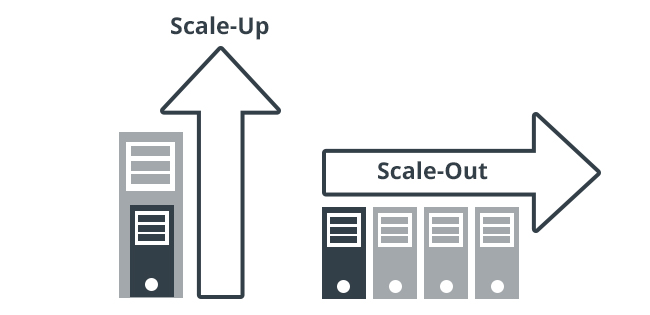
\includegraphics[width=0.7\textwidth]{resources/scales}
\caption[TEST]{TEST\protect\footnotemark}
\label{img:scales}
\end{figure}
\footnotetext{TEST: \url{https://magazin.kapilendo.de/den-supergau-verhindern-so-bereiten-sie-ihre-website-auf-einen-besucheransturm-vor/}, zugegriffen am 15. Januar 2017}

\section{Allgemein} \clearpage
%\chapter{NoSQL-Systemen}
%\begin{tikzpicture}[remember picture,overlay]
%\node[anchor=east,inner sep=0pt] at (current page text area.east|-0,6cm) %{
\includegraphics[height=4cm]{resources/mongoDBlogo}};
%\end{tikzpicture}
\section{Definition}
Im Vergleich zu den relationalen Datenbanken, die sich als eine strukturierte Sammlung von Tabellen (den Relationen) vorstellen, in welchen Datensätze abgespeichert sind, eignen sich NoSQL Datenbanken zur unstrukturierter Daten, die einen nicht-relationalen Ansatz verfolgen. Typische Beispiele für unstrukturierte Daten sind: Benutzer- und Sitzungsdaten, Chat-, Messaging- und Protokolldaten, Zeitreihendaten wie IoT- und Gerätedaten sowie große Objekte wie Videos und Bilder.\footnote{NSQL-Datenbanken: \url{http://de.basho.com/resources/nosql-databases/}, zugegriffen am 20. Dezember 2016}

Der Begriff NoSQL steht nicht für 'kein SQL', sondern für 'nicht nur SQL' (Not only SQL). Das Ziel von NoSQL ist, relationale Datenbanken sinnvoll zu ergänzen, wo sie Defizite aufzeigen. Entstanden ist dieses Konzept in erster Linie als Antwort zur Unflexibilität, sowie zur relativ schwierigen Skalierbarkeit von klassischen Datenbanksystemen, bei denen die Daten nach einem stark strukturierten Modell gespeichert werden müssen.\footnote{MySQL vs. MongoDB: \url{http://www.computerwoche.de/a/datenbanksysteme-fuer-web-anwendungen-im-vergleich,2496589}, zugegriffen am 22. Dezember 2016} Dokumentdatenbanken gruppieren die Daten in einem strukturierten Dokument, typischerweise in einer JSON-Datenstruktur. Auch MongoDB, siehe dazu Kapitel \ref{mongo} verfolgt diesen Ansatz und bietet darauf aufbauend eine reichhaltige Abfragesprache und Indexe auf einzelne Datenfelder. Die Möglichkeiten der Replikation und des Shardings zur stufenlosen und unkomplizierten Skalierung der Daten und Zugriffe macht MongoDB auch für stark frequentierte Websites äußerst interessant.(\cite{Hollosi.2012}, Kapitel 14, Seite 435)
\subsection{Kategorisierung von NoSQL-Systemen}
Der Abschnitt stellt verschiedene NoSQL-Systemen mit ihren Vor- und Nachteilen vor.
\subsubsection{Dokumentenorientierte Datenbanken}

Siehe Artikel \url{http://pi.informatik.uni-siegen.de/Mitarbeiter/mrindt/Lehre/Seminare/NoSQL/einreichungen/NOSQLTEC-2015_paper_9.pdf}

siehe \cite[S. 5-8]{Edlich.2011}
\subsubsection{Key-Value-Datenbanken}
\subsubsection{Spaltenorientierte Datenbanken}
\subsubsection{Objektdatenbanken}
\subsubsection{Graphdatenbanken}

\section{ACID}
bla

\section{Das CAP-Theorem}


Im Jahr 2000 hielt Brewer\footnote{Eric A. Brewer ist ein Informatik-Professor an der University of California, Berkeley und einer der Erfinder der Suchmaschine Inktomi} die Keynote auf dem ACM Symposium on Principles of Distributed Computing (PODC)\footnote{PODC2000: \url{http://www.podc.org/podc2000/}, zugegriffen am 02.01.2017}, einer Konferenz über die Grundlagen der Datenverarbeitung in verteilten Systemen\footnote{In einem verteilten System im Bereich Datenverarbeitung werden gespeicherte Daten mehrfach über mindestens zwei verschiedene Server repliziert und miteinander synchronisiert, um die Verfügbarkeit der Daten zu erhöhen und die Zugriffszeiten der User zu verringern.} (Principles of Distributed Computing).  In seiner Keynote stellte Brewer sein \textbf{CAP}-Theorem vor, ein Ergebnis seiner Forschungen zu verteilten Systemen an der University of California \cite[S. 13]{Kurowski.2012}. Brewer's Theorem wurde im Jahr 2002 von Seth Gilbert und Nancy Lynch formal bewiesen.

Das Akronym \textbf{CAP} steht für die englischsprachigen Begriffe  \Cap, \cAp\ und \caP\ und beschreiben die Anforderungen für die Skalierung an verteilte Systeme, die es zunächst näher zu erläutern gilt.

Was besagt eigentlich dieses \textbf{CAP}-Theorem? Das \textbf{CAP}-Theorem besagt, dass die verteilten Systeme, die mit großen Datenmengen zu tun haben, gleichzeitig die folgenden Anforderungen wie \Cap, \cAp\ und \caP\ nicht erfüllen können.
%\begin{figure}
%\centering
%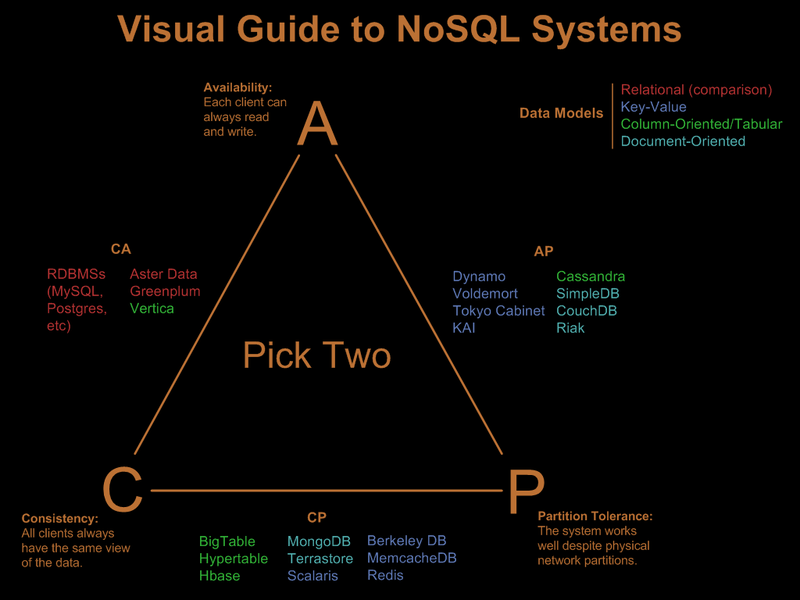
\includegraphics[width=1.0\textwidth]{resources/pickTwoCAP}
%\caption[bla]{CAP Theorem\protect\footnotemark}
%\label{img:cap}
%\end{figure}
%\footnotetext{Visual Guide to NoSQL Systems: \url{http://blog.nahurst.com/visual-guide-to-nosql-systems}, zugegriffen am 27. Dezember 2016}
%\begin{figure}
%\centering
%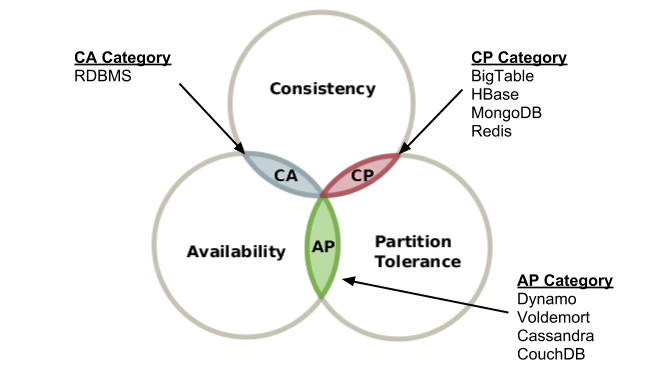
\includegraphics[width=0.8\textwidth]{resources/captheorem2}
%\caption[\capTheorem]{Anforderungen an verteilte Systeme gemäß dem Professor Eric A. Brewer's \capTheorem\protect\footnotemark}
%\label{img:cap}
%\end{figure}
%\footnotetext{CAP Theorem: \url{https://datawarehouseview.wordpress.com/tag/cap-theorem/}, zugegriffen am 23. Dezember 2016}
%

\begin{figure}
\centering
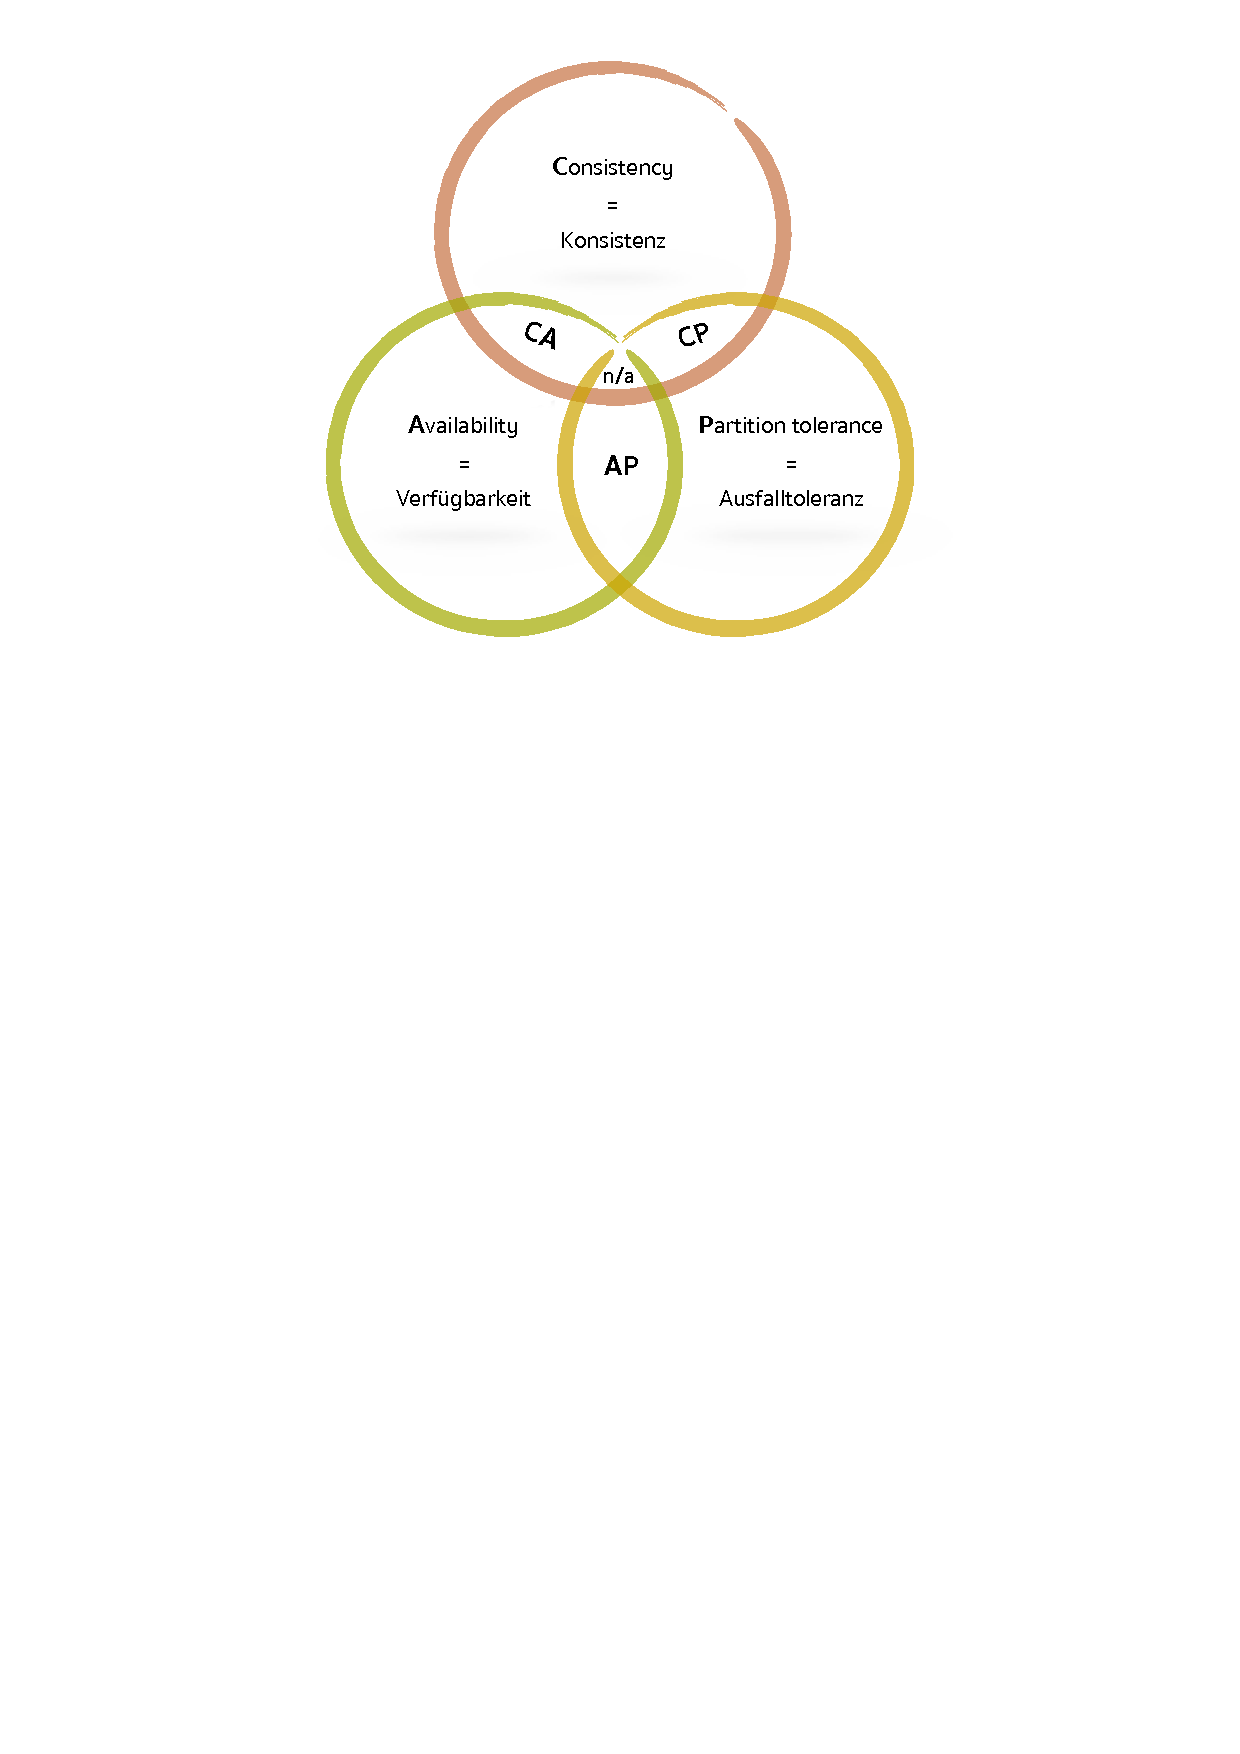
\includegraphics[trim = 0mm 189mm 0mm 9mm, clip, width=1.0\textwidth]{resources/myPictureForCAP}
\caption[\textbf{CAP}-Theorem]{Anforderungen an verteilte Systeme gemäß dem \textbf{CAP}-Theorem}
\label{img:cap}
\end{figure}

%\begin{figure}
%\centering
%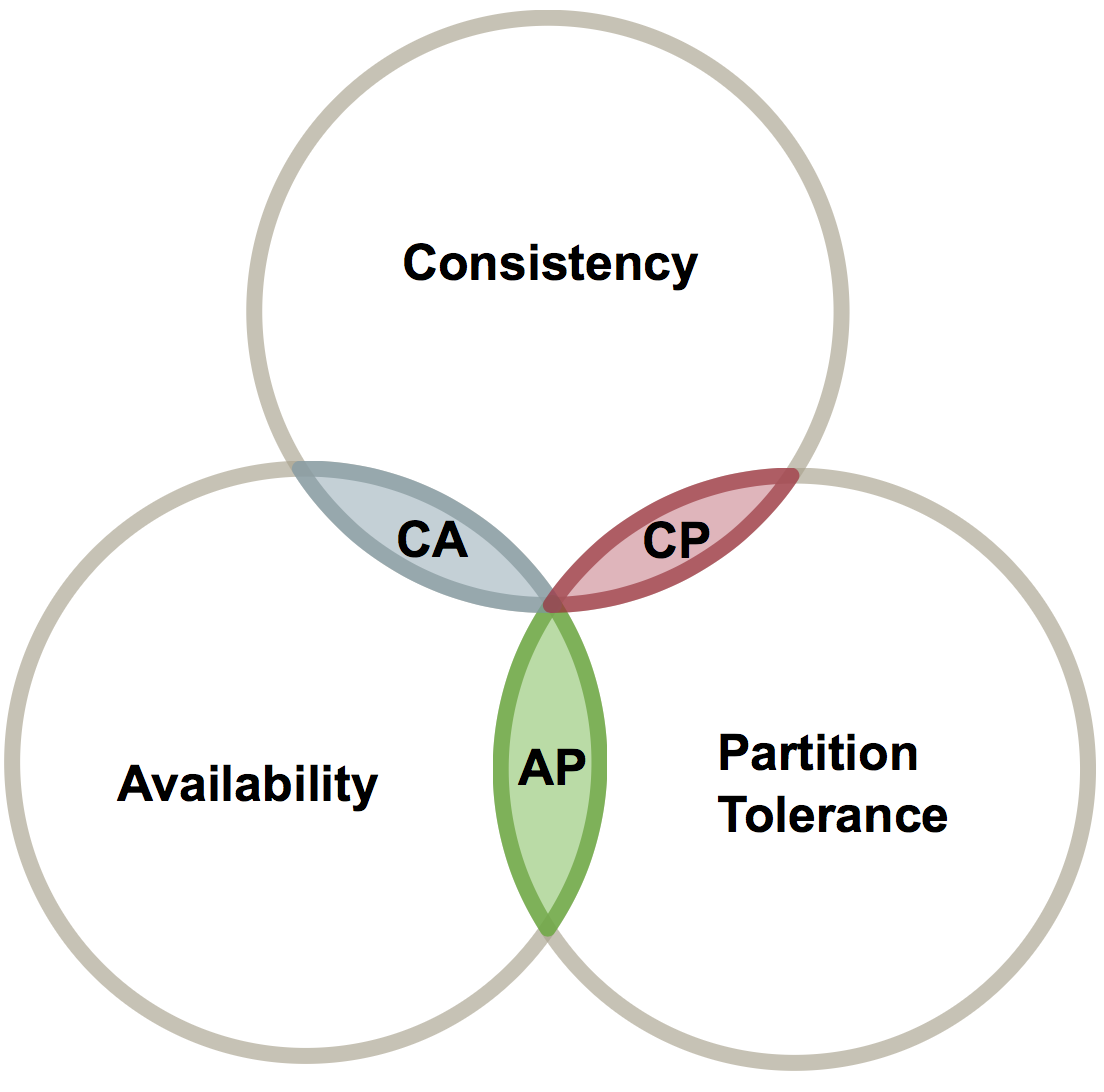
\includegraphics[width=0.5\textwidth]{resources/cap}
%\caption[bla]{CAP Theorem \protect\cite{Brewer.}}
%\label{img:cap}
%\end{figure}

\begin{itemize}
\item \Cap: Die \textit{Konsistenz} der Daten in einem verteilten System bedeutet, dass alle replizierenden Knoten aus einem großen Cluster über die gleiche Datenstruktur verfügen. Falls ein Wert auf einem Knoten durch eine Transaktion per Schreiboperation geändert ist, muss der aktualisierte Wert auf Anfrage mit der Leseoperation von anderen Knoten zurückgeliefert werden können. Die Transaktion selbst ist eine atomare\footnote{Eine atomare Transaktion bedeutet, dass sie entweder ganz oder gar nicht ausgeführt wird. Falls eine atomare Transaktion abgebrochen wird, werden alle im Laufe der Transaktion schon durchgeführte Änderungen rückgängig gemacht.} Einheit in der Datenbank.
%
%\item \Cap: Die \textit{Konsistenz} der gespeicherten Daten beschreibt in einem verteilten Datenbanksystem so einen Datenstand auf den Servern, in dem nach dem Abschluss einer Transaktion alle replizierenden Knoten aus einem großen Cluster über die gleiche Datenstruktur verfügen. Die Transaktion selbst ist eine atomare Einheit in der Datenbank, die entweder als Ganzes erfolgreich verläuft \textbf{(=Commit)} oder durch einen \textbf{Rollback} rückgängig gemacht werden kann.
%
%\textbf{Beispiel für einen konsistenten Zustand der gespeicherten Daten:} In einem verteilten Datenbanksystem mit mehreren replizierenden Knoten sind die Daten nur dann konsistent, wenn auf einem Knoten geänderte Eintrag die alle darauf folgenden Lesezugriffe über andere Cluster den geänderten Wert zurückliefert.
%
%ändert sich nach einer Transaktion auf einem Knoten ein Eintrag in einem Dokument. Um alle folgenden Lesezugriffe, die beispielsweise über andere Knoten aus demselben Cluster ausgeführt w
%
%für einen konsistenten Zustand ändert eine Transaktion in einem Knoten einen Datensatz. Bei erfolgreichem Abschluss der Transaktion muss der geänderte Wert in einem verteilten Datenbanksystem mit mehreren replizierenden Knoten bei der Anfrage von jedem Knoten zurückgeliefert werden können.
%
\item \cAp: Die \textit{Hochverfügbarkeit} ist die weitere Anforderung, die besagt, dass immer alle gesendeten Anfragen durch User ans System beantwortet werden müssen und mit einer akzeptablen Reaktionszeit.
\item \caP: Die \textit{Partitions- oder Ausfalltoleranz} bedeutet, dass der Ausfall eines Knoten bzw. eines Servers aus einem Cluster das verteilte System nicht beeinträchtigt und es fehlerfrei weiter funktioniert. Falls einzelne Knoten in so einem System ausfallen, wird deren Ausfall von den verbleibenden Knoten aus dem Cluster kompensiert, um die Funktionsfähigkeit des Gesamtsystems aufrecht zu halten.

\end{itemize}

Die graphische Darstellung für das Brewer's \textbf{CAP}-Theorem ist aus der Abbildung \ref{img:cap} zu entnehmen. Wie die Abbildung \ref{img:cap} erkennen lässt, können in einem verteilten System gleichzeitig und vollständig nur zwei dieser drei Anforderungen  \Cap, \cAp, \caP\ erfüllt sein. Konkret aus der Praxis bedeutet das, dass es für eine hohe Verfügbarkeit und Partitions- oder Ausfalltoleranz notwendig ist, die Anforderungen an die Konsistenz zu lockern \cite[S. 31]{Edlich.2011}.

Die Anforderungen in Paaren klassifizieren gemäß dem \textbf{CAP}-Theorem bestimmte Datenbanktechnologien. Für jede Anwendung muss daher individuell entschieden werden, ob sie als ein \textbf{CA-}, \textbf{CP-} oder \textbf{AP-}System zu realisieren ist.
\begin{itemize}
\item \textbf{CA} (\textbf{C}onsistency und \textbf{A}vailability): Die klassischen relationalen Datenbankmanagementsysteme (RDBMS) wie Oracle, DB2 etc. fallen in \textbf{CA}-Kategorie, die vor allem \Cap\ und \cAp\ aller Knoten in einem Cluster hinzielt. Hierbei werden die Daten nach dem \textbf{ACID}-Prinzip verwaltet. Die relationalen Datenbanken sind für Ein-Server-Hardware konzipiert und vertikal skalierbar. Das bedeutet, dass solche Systeme mit hochverfügbaren Servern betrieben werden und \caP\  nicht unbedingt in Frage kommt.

\item \textbf{CP} (\textbf{C}onsistency und \textbf{P}artition tolerance): Ein gutes Beispiel für die Anwendungen, die zu der \textbf{CP-}Kategorie zu zuordnen sind, sind Banking-Anwendungen. Für solche Anwendungen ist es wichtig, dass die Transaktionen zuverlässig durchgeführt werden und der mögliche Ausfall eines Knotens sichergestellt wird.

\item \textbf{AP} (\textbf{A}vailability und \textbf{P}artition tolerance): Für die Anwendungen, die in die \textbf{AP-}Kategorie fallen, rückt die Anforderung \Cap\ in den Hintergrund. Beispiele für solche Anwendungen sind die Social-Media-Sites wie Twitter\footnote{Twitter: \url{https://twitter.com/}} oder Facebook\footnote{Facebook: \url{https://www.facebook.com/}}, da die Hauptidee der Anwendung dadurch nicht verfällt, wenn zum gleichen Zeitpunkt die replizierten Knoten nicht über die gleiche Datenstruktur verfügen. 
\end{itemize}

\section{BASE}

\begin{itemize}
\item \textbf{B}asically \textbf{A}vailable: bla

\item \textbf{S}oft State: bla

\item \textbf{E}ventual consistency: bla
\end{itemize}

\section{MongoDB}\label{mongo}
Die nicht-relationale Datenbank 'MongoDB' macht mit einem effizienten Dokument-orientierten Ansatz, einfacher Skalierbarkeit und hoher Flexibilität dem bewährten MySQL\footnote{MySQL: \url{https://www.mysql.com}}-System zunehmend Konkurrenz.\footnote{MySQL vs. MongoDB: \url{http://www.computerwoche.de/a/datenbanksysteme-fuer-web-anwendungen-im-vergleich,2496589}, zugegriffen am 19. Dezember 2016}

\subsection{Einleitung}
Das System 'MongoDB' wurde 2009 vom amerikanischen Startup 10gen nach rund zwei Jahren Entwicklung der Öffentlichkeit als Open-Source-Lösung vorgestellt. Der etwas gewöhnungsbedürftige Name stammt von dem englischen Begriff "humongous", der sich ins Deutsche mit 'gigantisch'  beziehungsweise "riesig" übersetzen lässt. Die Lösung basiert auf der Programmiersprache C++ und ist für die Betriebssysteme Windows, Mac OS X und Linux erhältlich. Sowohl 32-Bit- als auch 64-Bit-Systeme werden unterstützt. Wie der Hersteller erklärt, ist die Lösung auf starke Leistung, große Datenmengen, hohe Flexibilität sowie einfache Skalierbarkeit ausgelegt.\footnote{MySQL vs. MongoDB: \url{http://www.computerwoche.de/a/mysql-vs-mongodb-datenbanksysteme-im-vergleich,1233517}, zugegriffen am 22. Dezember 2016}

Die MongoDB ist eine Open-Source Software, die unter einer Apache Lizenz veröffentlicht wird. 

\subsection{Tabellen haben ausgedient - Dokumente als Datensätze}
\textbf{ Dokumentenorientierte Datenbanken speichern Daten nicht in Form von Tabellen, sondern in Form von Dokumenten. Im Fall der MongoDB handelt es sich um Dokumente im JSON-ähnlichen Format Binary JSON oder BSON.}
Die nicht-relationale Datenbank MongoDB speichert Datensätze in Form von Dokumenten im BJSON\footnote{BJSON: \url{http://www.bjson.org}}-Format. Statt von Tabellen spricht man bei MongoDB von Kollektionen (Collections). Jede Kollektion kann Dokumente beinhalten analog zu Zeilen beziehungsweise Datensätzen in einer MySQL-Tabelle. Dokumente werden im so genannten BSON-Format gespeichert und ausgegeben. Sie sind dann Javascript-Objekten sehr ähnlich. Das Format stammt von dem kompakten JSON-Format (Javascript Object Notation) ab und ist, wie das Präfix 'Binary' (Binary JSON = BSON) andeutet, für eine Overhead-arme Darstellung von binären Datenobjekten ausgelegt. Jedes Dokument kann dabei eine beliebige Anzahl an Feldern besitzen, während eine verschachtelte Array-Struktur ebenfalls möglich ist. Zudem dürfen Dokumente auch innerhalb eines Dokuments gespeichert werden.\footnote{Siehe in Deutsch: \url{https://www.iks-gmbh.com/assets/downloads/Einfuehrung-in-MongoDB-iks.pdf}, zugegriffen am 19. Dezember 2016}

Der entscheidende Unterschied zu relationalen Datenbanken besteht darin, dass MongoDB als NoSQL-Datenbank dokumentenorientiert arbeitet. Dokumentenbasierende Datenbanken sind auf eine schemafreie Struktur ausgelegt. Bei MongoDB gibt es also kein festes Tabellenschema und dadurch beispielsweise auch keine zwingenden Relationstabellen und "Joins", die mit der Weiterentwicklung und dem Ausbau der Datenbank immer komplexer werden. Stattdessen lassen sich Relationen entweder direkt im Datensatz speichern oder bei Bedarf individuell bei der Datenabfrage erstellen. Dadurch ist die Datenstruktur wesentlich flexibler als bei MySQL und lässt sich einfach horizontal skalieren.

\subsection{Architektur}
Zu den wichtigsten Eigenschaften, die für einen Einsatz von MongoDB sprechen, gehören:
\begin{itemize}
\item Hochverfügbarkeit: Auch bei Ausfall einer Datenbankinstanz soll die Applikation weiterhin verfügbar bleiben, d. h. nahtlos – ohne manuellen Eingriff – müssen redundante Instanzen bei einem Ausfall einspringen
\item Skalierbarkeit: Mit transparentem Sharding, siehe Kapitel \ref{sharding} – einem Verfahren zur horizontalen Skalierung – kann die Infrastruktur vergleichsweise einfach wachsenden Anforderungen angepasst werden
\item Performanz: Vom Ansatz her haben dokumentenorientierte DBMS hier einen Vorteil, weil die Daten nicht erst aus mehreren Tabellen zusammengeführt werden\footnote{MongoDB Eigenschaften: \url{https://entwickler.de/online/datenbanken/mongodb-erfolgreich-ein-dokumentenorientiertes-datenbanksystem-einfuehren-115079.html}, zugegriffen am 12. Dezember 2016}
\end{itemize}

Die Vorteile relationaler und NoSQL-Datenbanken sind aus der Abbildung \ref{img:architektur} zu entnehmen.
\begin{figure}
\centering
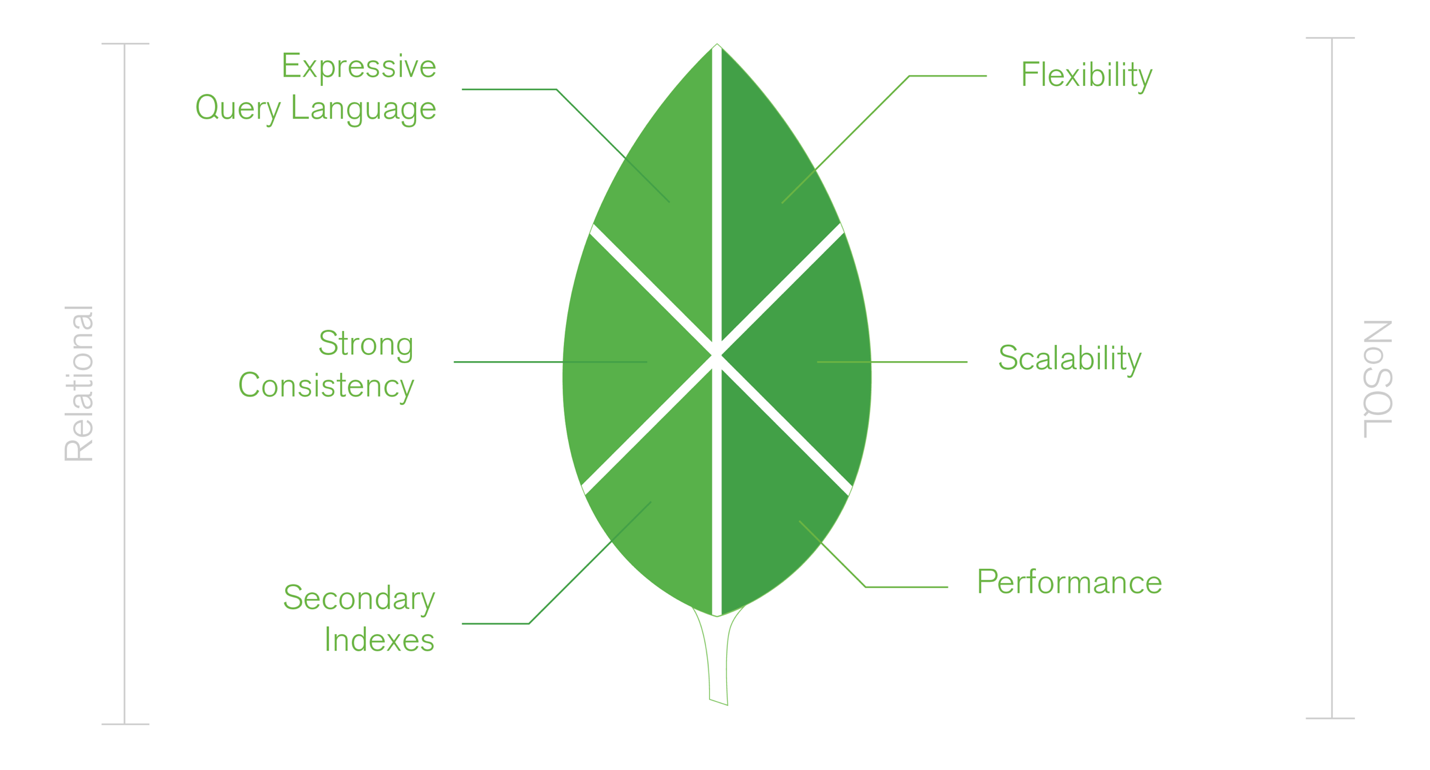
\includegraphics[width=0.9\textwidth]{resources/architectureNoSQLVSRelational}
\caption[MongoDB Architektur]{MongoDB Architektur\protect\footnotemark}
\label{img:architektur}
\end{figure}
\footnotetext{MongoDB Architektur: \url{http://www.moretechnology.de/mongodb-eine-dokumentenorientierte-datenbank/}, zugegriffen am 23. Dezember 2016}

\subsection{CRUD/IFUR}
\subsubsection{Create/Insert}
\begin{listingsboxShell}[label={lst:insert}]{myshell}{Dokument speichern}
> db.collection.insert(..)
\end{listingsboxShell}
\subsubsection{Read/Find}
\begin{listingsboxShell}[label={lst:find}]{myshell}{Dokument finden}
> db.collection.find(..)
> db.collection.findOne(..)
\end{listingsboxShell}
\subsubsection{Update/Update}
\begin{listingsboxShell}[label={lst:update}]{myshell}{Dokument aktualisieren}
> db.collection.update(..)
\end{listingsboxShell}
\subsubsection{Delete/Remove}
\begin{listingsboxShell}[label={lst:remove}]{myshell}{Dokument löschen}
> db.collection.remove(..)
\end{listingsboxShell}
\subsection{Schema Design}
\subsection{Performance}
Siehe in Deutsch über Indexes: \url{https://books.google.de/books?id=kRUbDAAAQBAJ&pg=PA53&lpg=PA53&dq=index+in+mongodb+was+ist+da&source=bl&ots=80Kgw664kZ&sig=rEhHo3g4JRVAVXwUr_In5xzWB8c&hl=en&sa=X&ved=0ahUKEwiBvd_VsbfQAhVDtBQKHX4_ASAQ6AEINjAC#v=onepage&q=index%20in%20mongodb%20was%20ist%20da&f=false}\newline

\subsection{Aggregation Framework}

\subsection{Sharding}\label{sharding}
MongoDB bietet mit AutoSharding ein Feature, das es ermöglicht, einen Datenbankserver automatisch auf verschiedene physikalische Maschinen aufzuteilen und somit die Datenbank horizontal zu skalieren. Um das Sharding bei MongoDB zu konfigurieren, werden drei Komponenten benötigt...., siehe Sharding \url{https://www.iks-gmbh.com/assets/downloads/Einfuehrung-in-MongoDB-iks.pdf
}

\subsection{ODMs für MongoDB}

ODM ist Object-Document Mapper für nichtrelationale Datenbanken wie MongoDB, Apache Cassandra etc.

\subsubsection{Morphia}
Morphia is the Java Object Document Mapper for MongoDB \url{http://mongodb.github.io/morphia/}

\subsubsection{Doctrine}
The Doctrine MongoDB ODM project is a library that provides a PHP object mapping functionality for MongoDB. \url{https://github.com/doctrine/mongodb-odm}

\subsection{Beziehungen}
Folgenden Relationen wie One-to-One \textbf{Teilabschnitt \ref{1:1}}, One-to-Many \textbf{Teilabschnitt \ref{1:n}} und Many-to-Many \textbf{Teilabschnitt \ref{n:m}} blabla

\subsubsection{One-to-One}\label{1:1}
bla

\subsubsection{One-to-Many}\label{1:n}
bla

\subsubsection{Many-to-Many}\label{n:m}
bla

\subsection{Storage Engines}

\subsubsection{MMAPv1}
MMAPv1 is default a storage engine.
MMAPv1 automatically allocates power-of-two-sized documents when new documents are inserted
This is handled by the storage engine.
MMAPv1 is built on top of the mmap system call that maps files into memory
This is the basic idea behind why we call it MMAPv1.

\subsubsection{WiredTiger}

\begin{listingsboxShell}[label={lst:X}]{myshell}{Alle mongod-Prozesse zwingend stoppen}
> killall mongod
\end{listingsboxShell}

Für den Wahl des Storage-Engines \textbf{Wired Tiger} muss man im Terminal den Befehl aus Listing \ref{lst:wiredTiger} ausführen.

\begin{listingsboxShell}[label={lst:wiredTiger}]{myshell}{Something else}
> mongod -dbpath WT --storageEngine wiredTiger
\end{listingsboxShell}

Dann mongo starten mit 'mongo', dann:

\begin{listingsboxShell}[label={lst:X}]{myshell}{Something else}
> db.foo.insert({'name':'andrew'})
\end{listingsboxShell}

\begin{listingsboxShell}[label={lst:X}]{myshell}{Something else}
> db.foo.stats()
\end{listingsboxShell}

\subsection{Indizes}
Indizes in MongoDB werden als Binär-Baum\footnote{Binär-Baum: \url{http://www.hs-augsburg.de/mebib/emiel/entw_inf/lernprogramme/baeume/gdi_kap_4_1.html}, zugegriffen am 23. Dezember 2016} in einer vordefinierten Sortierreihenfolge abgelegt, siehe Abbildung \ref{img:IndexesInMongoDBAreB-Trees}

Der Index wird beim Erstellen, Updaten und Löschen eines Dokumentes auch aktualisiert. Zu viele Indizes machen schreib Operationen langsam und die Größe der Indizes steigt an, deswegen sollte ein Index nur auf Felder zeigen, auf die auch Query-Operationen angewendet werden. Beim Anlegen der Indizes ist die Sortierreihenfolge zu gunsten einer schnelleren Suche wichtig, da sie schon vorsortiert vorliegen und nicht erst bei der Liveabfrage sortiert werden müssen.\footnote{Indizes: \url{http://wikis.gm.fh-koeln.de/wiki_db/MongoDB/Indizes}, aufgerufen am 24. Dezember 2016}

Es gibt drei Möglichkeiten der Sortierung:

\begin{itemize}
\item Aufsteigend(1),
\item Absteigend (-1),
\item geospatial (2d).
\end{itemize}

Index hilft, Datenbanken zu optimieren. Die nachfolgende \autoref{img:EfficiencyofIndexUse} demonstriert

\begin{figure}
\centering
	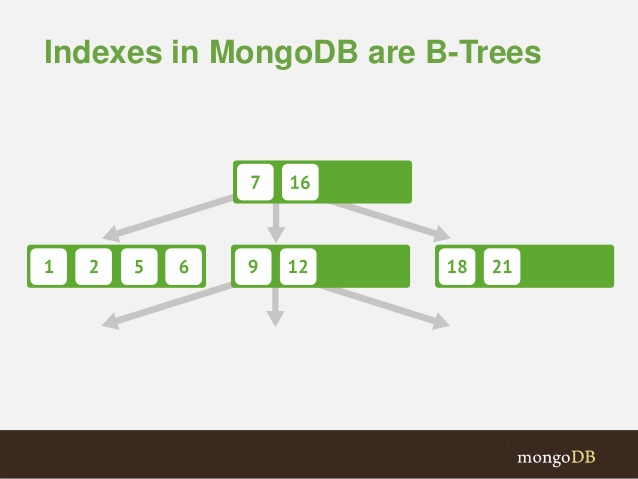
\includegraphics[width=0.7\textwidth]{resources/indexingBtree}
\caption[Indizes in MongoDB als Binär-Baum]{Indizes in MongoDB als Binär-Baum\protect\footnotemark}
\label{img:IndexesInMongoDBAreB-Trees}
\end{figure}
\footnotetext{Indizes in MongoDB als Binä
r-Baum: \url{http://www.slideshare.net/mongodb/indexing-strategies-to-help-you-scale}, zugegriffen am 23. Dezember 2016}

blabla

\begin{figure}
\centering
	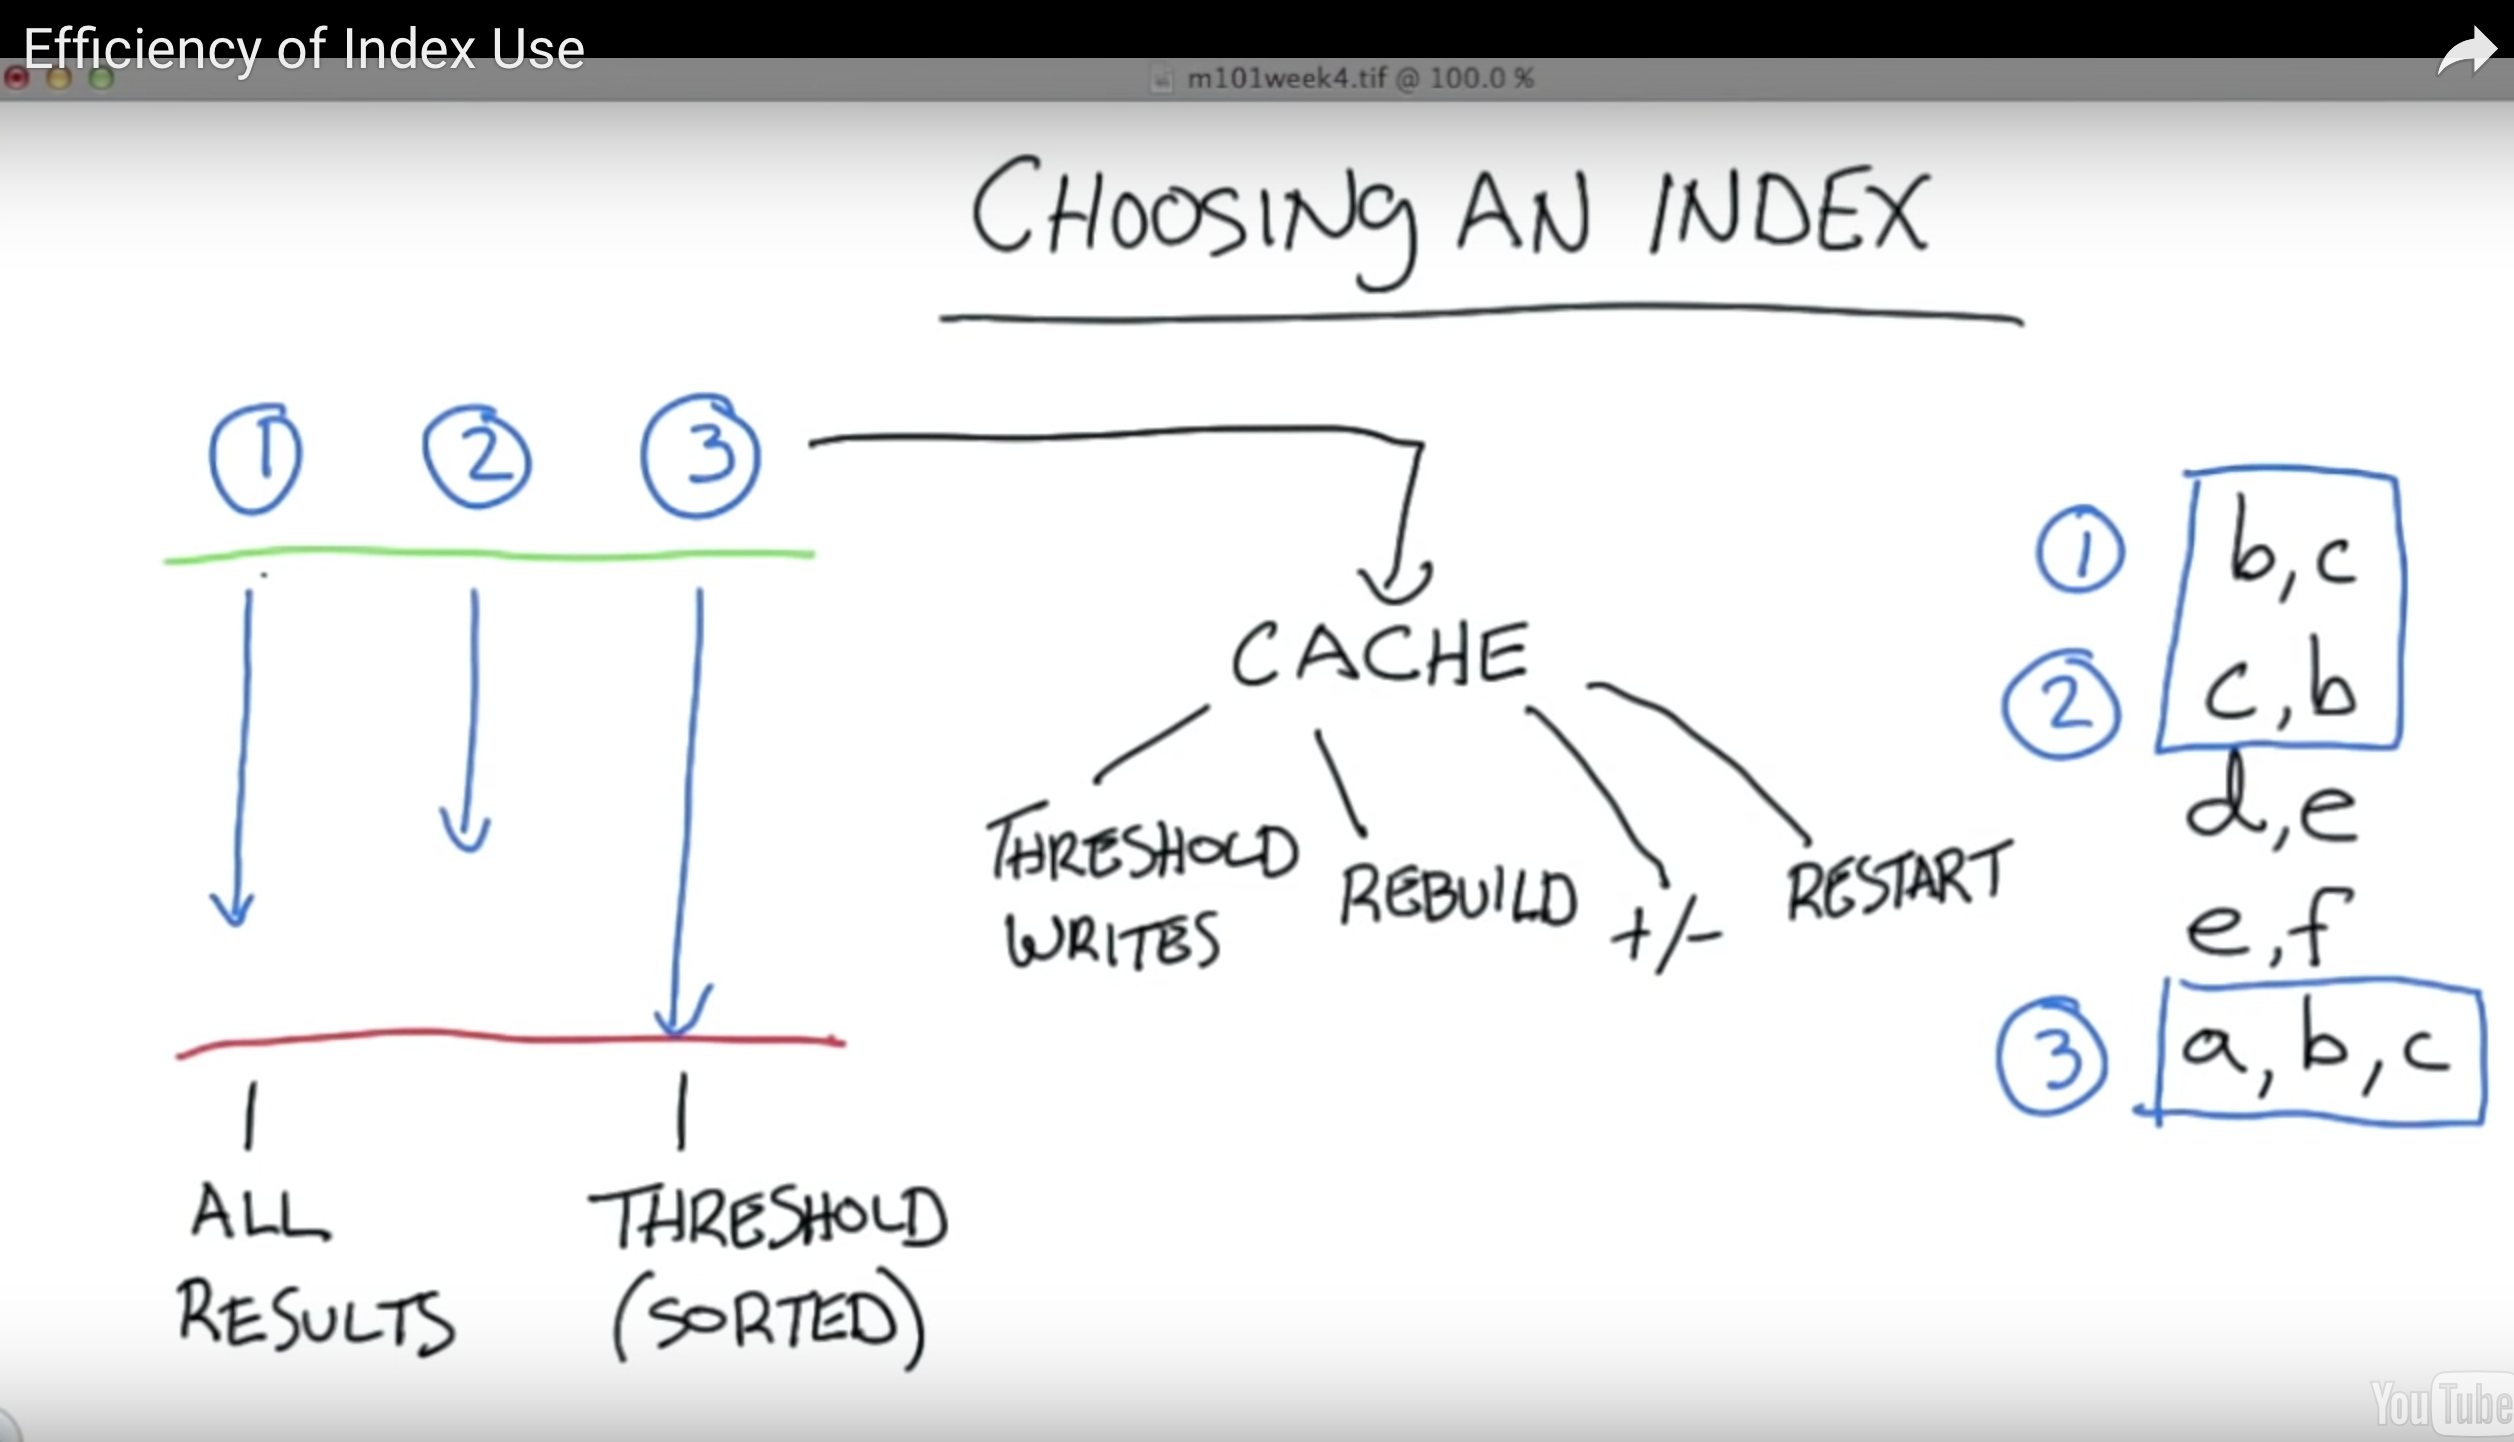
\includegraphics[width=0.7\textwidth]{resources/efficiencyOfIndexUse}
\caption[Efficiency of Index Use]{Efficiency of Index Use\protect\footnotemark}
\label{img:EfficiencyofIndexUse}
\end{figure}
\footnotetext{Efficiency of Index Use: \url{https://docs.mongodb.com/manual/indexes/}, zugegriffen am 12. Dezember 2016}


Neben dem obligatorischen Primär-Index auf dem Feld \_id, das in jedem Dokument existieren und pro Collection eindeutig sein muss, können Sie in MongoDB bis zu 63 weitere Sekundär-Indizes pro Collection anlegen, um Suchanfragen zu beschleunigen. Ein Sekundär-Index kann auf einem einzelnen Feld oder einer Gruppe von Feldern angelegt werden.%\footnote{Indizes: \url{https://www.informatik-aktuell.de/betrieb/datenbanken/mongodb-fuer-software-entwickler.html}}

Which optimization will typically have the greatest impact on the performance of a database?\newline
Adding appropriate indexes on large collections so that only a small percentage of queries need to scan the collection.

\subsection{Creating Indexes}
blabla

\begin{listingsboxShell}[label={lst:X}]{myshell}{Mongo-Shell: Something else}
> db.students.createIndex();
\end{listingsboxShell}

blabla

\begin{listingsboxShell}[label={lst:X}]{myshell}{Mongo-Shell: Something else}
> db.students.explain().find();
\end{listingsboxShell}

Quiz: Please provide the mongo shell command to add an index to a collection named students, having the index key be class, student\_name.
Neither will go in the "-1" direction..

\begin{listingsboxShell}[label={lst:X}]{myshell}{Something else}
> db.students.createIndex({student\_name:1, class:1});
\end{listingsboxShell}

\begin{listingsboxShell}[label={lst:X}]{myshell}{Mongo-Shell: Something else}
> db.students.dropIndex({student_name:1});
\end{listingsboxShell}

\subsubsection{Multikey Indexes}
blabla
\subsubsection{Index Creation Option, Unique}
für jedes attribut kann man Unique definieren, d.h. doppelte Werte dürfen nicht vorkommen\newline\newline

\begin{listingsboxShell}[label={lst:X}]{myshell}{Mongo-Shell: Something else}
> db.students.createIndex({student_id : test}, {unique:true});
\end{listingsboxShell}

Please provide the mongo shell command to create a unique index on student\_id, class\_id, ascending for the collection students.

\begin{listingsboxShell}[label={lst:X}]{myshell}{Mongo-Shell: Something else}
> db.students.createIndex({student_id:1, class_id:1}, {unique:true});
\end{listingsboxShell}

\subsubsection{Index Creation, Sparse}

Im Fall, wenn ein Attribut nicht in allen Dokumenten vorkommt, aber für dieses ein Unique Index definiert werden soll, muss Folgendes verwendet werden:

\begin{listingsboxShell}[label={lst:X}]{myshell}{Something else}
> db.students.createIndex({cell:1}, {unique:true, sparse:true});
\end{listingsboxShell}

blabla, siehe den Shellbefehl, blabla

\begin{listingsboxShell}[label={lst:X}]{myshell}{Something else}
> db.students.createIndex({student_id:1, class_id:1}, {unique:true});
\end{listingsboxShell}
siehe Codeauszug 

\section{Prototyp}
Kommentare zu den Fotos hinzufügen, Eingebettete Kommentare, siehe \url{http://ezproxy.bib.fh-muenchen.de:2125/doi/pdf/10.3139/9783446431225.014}

\section{Aggregation Framework}
How good is it? Mapping between SQL and Aggregation
Um die Nutzung der Aggregation Framework in MongoDB zu ermöglichen, stellt MongoDB Java Driver zur Verfügung. 

\section{Replikation und Verfügbarkeit}
MongoDB kann Server in Replikationsgruppen anordnen, damit bei Ausfall eines Servers die Verfügbarkeit der Datenbank trotzdem gewährleistet ist. In diesem Kapitel werden die Konfigurationsmöglichkeiten für Replikation und Verfügbarkeit der Daten veranschaulicht und zwar wie man Replikation und Verfügbarkeit in MongoDB konfiguriert.
\subsection{Replikation (=Replication)}
blabla

\begin{figure}
\centering
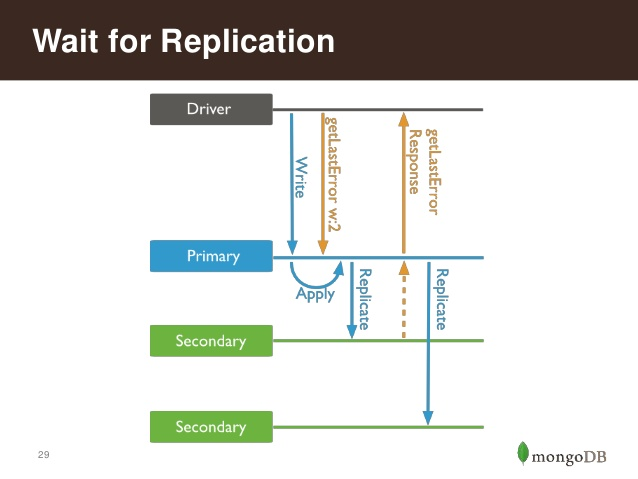
\includegraphics[width=0.7\textwidth]{resources/replication}
\caption[Replikation]{Replikation\protect\footnotemark}
\label{img:Replikation}
\end{figure}
\footnotetext{Replikation: \url{http://www.slideshare.net/mongodb/webinarserie-einfhrung-in-mongodb-back-to-basics-teil-3-interaktion-mit-der-datenbank}, zugegriffen am 18. Dezember 2016}

blabla
\begin{figure}
\centering
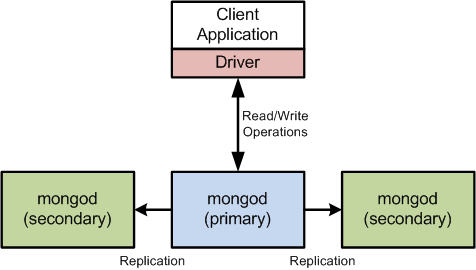
\includegraphics[width=0.7\textwidth]{resources/mongo_replication}
\caption[Master-slave replication in MongoDB]{Master-slave replication in MongoDB\protect\footnotemark}
\label{img:mongo_replication}
\end{figure}
\footnotetext{Master-slave replication in MongoDB: \url{http://spichale.blogspot.de/2013/08/replication-in-mongodb-concepts-and.html}, zugegriffen am 29. Dezember 2016}



Typen von Replikationsgruppen:
\begin{itemize}
\item Regular
\item Arbiter
\item Delayed/Regular
\item Hidden
\end{itemize}
\subsection{Erstellen von Replikationsgruppen}

\begin{listingsboxShell}[label={lst:scriptForCreateOfRep}]{myshell}{Skript fürs Erstellen einer Replikationsgruppe}
#!/usr/bin/env bash

mkdir -p /data/rs1 /data/rs2 /data/rs3

// Start von drei lokalen mongod-Instanzen als Replikationsgruppe

mongod --replSet m101 --logpath "1.log" --dbpath /data/rs1 --port 27017
--oplogSize 64 --fork --smallfiles
mongod --replSet m101 --logpath "2.log" --dbpath /data/rs2 --port 27018
--oplogSize 64 --smallfiles --fork
mongod --replSet m101 --logpath "3.log" --dbpath /data/rs3 --port 27019
--oplogSize 64 --smallfiles --fork
\end{listingsboxShell}

Das Skript mit dem Inhalt aus Listing \ref{lst:scriptForCreateOfRep} ist mit dem aus Listing \ref{lst:runOfscriptForCreateOfRep} auszuführen:

\begin{listingsboxShell}[label={lst:runOfscriptForCreateOfRep}]{myshell}{Erstellen einer Replikationsgruppe anhand eines Skriptes}
vlfa:scripts vlfa$ bash < create_replica_set.sh
\end{listingsboxShell}

Bei der Ausführung des Skriptes kann zu den Problemen führen. Um aktuelle Prozesse mit mongo anschauen und stoppen zu können, muss man folgenden Befehl angeben. The problem was that I have runned mongod without any parameters before I started launching the nodes. First kill all the mongo, mongod and mongos instances to guarantee the environment is clear.\url{http://stackoverflow.com/questions/25839559/mongodb-server-is-not-running-with-replset}

\begin{listingsboxShell}[label={lst:listOfPIDs}]{myshell}{Auflistung aktueller mongo(s,d)-Prozesse}
vlfa:scripts vlfa$ ps -ef | grep 'mongo'
\end{listingsboxShell}

Danach ist wichtig, Prozesse zu stoppen. Dafür muss man nach dem Befehl kill die ProzessID eingeben, siehe Listing \ref{lst:killPID}. Dann wird die Möglichkeit fürs Erstellen eigener Replikationsgruppe ermöglicht, siehe dazu Listings \ref{lst:scriptForCreateOfRep} und \ref{lst:runOfscriptForCreateOfRep}.

\begin{listingsboxShell}[label={lst:killPID}]{myshell}{mongo(s,d)-Server zwingend stoppen}
// konkreten mongo(s,d)-Server zwingend stoppen
vlfa:scripts vlfa$ kill 'PID'

// alle mongo(s,d)-Server zwingend stoppen
vlfa:scripts vlfa$ killall mongo(s,d)
\end{listingsboxShell}

Damit ist die Konfigurationsgruppe mit 3 Servern angelegt. Zum Anschauen einer log-Datei;

\begin{listingsboxShell}[label={lst:X}]{myshell}{1.log-Inhalt}
2016-12-19T14:58:11.637+0100 I CONTROL  [initandlisten] MongoDB starting :
pid=25626 port=27017 dbpath=/data/rs1 64-bit host=vlfa.fritz.box
// irrelevant
2016-12-19T14:58:11.639+0100 I CONTROL  [initandlisten] options:
{ net: { port: 27017 }, processManagement: { fork: true }, replication:
{ oplogSizeMB: 64, replSet: "m101" }, storage: { dbPath: "/data/rs1",
mmapv1: {smallFiles: true}}, systemLog: {destination: "file", path: "1.log"}}
// irrelevant
\end{listingsboxShell}
Die Replikationsgruppe starten.......blabla
\begin{listingsboxJavaScript}[label={lst:initReplica}]{myJS}{Skript zum Start der Replikationsgruppe}
config = { _id: "m101", members:[
          { _id : 0, host : "localhost:27017", priority:0, slaveDelay:5},
          { _id : 1, host : "localhost:27018"},
          { _id : 2, host : "localhost:27019"} ]
};

rs.initiate(config);
rs.status();
\end{listingsboxJavaScript}

Die Server aus Listing \ref{lst:initReplica} nehmen nun Kontakt miteinander auf, gründen die Gruppe und wählen den Primary-Server aus. Wie im Skript aus Listing 	\ref{lst:initReplica} zu entnehmen ist, kann der Zustand der Replikationsgruppe mit \texttt{rs.status()} geprüft werden. Bei Ausfall des Primary-Servers wählen die Secondaries untereinander entsprechend einen neuen Primary-Server. Damit wird die Ausfallsicherheit des Servers erreicht. Die Mindestanzahl an Server in einer Replikationsgruppe liegt bei drei. 

\begin{listingsboxShell}[label={lst:runOfInitReplica}]{myshell}{Skript ausführen}
vlfa:scripts vlfa$ mongo --port 27018 < init_replica.js
\end{listingsboxShell}

Die Priorität '0' teilt mit, wer Primary Member in der Replikationsgruppe ist. Korrigieren, Stimmt nicht....\url{https://docs.mongodb.com/v3.2/core/replica-set-priority-0-member/}

\begin{listingsboxJava}[label={lst:X}]{myJava}{Skript zur Initialisierung der Replikationsgruppe}
public static void main (String[] args) throws InterruptedException {
        MongoClient client = new MongoClient(asList(
                new ServerAddress("localhost", 27017),
                new ServerAddress("localhost", 27018),
                new ServerAddress("localhost", 27019)));
                
                // weitere Operationen
}
\end{listingsboxJava}

\begin{listingsboxShell}[label={lst:X}]{myshell}{Simulation des Server-Ausfalls 'PRIMARY'}
m101:PRIMARY> rs.stepDown()

Result:

2016-12-19T21:24:12.739+0100 I NETWORK  [thread1]
trying reconnect to 127.0.0.1:27018 (127.0.0.1) failed
2016-12-19T21:24:12.760+0100 I NETWORK  [thread1]
reconnect 127.0.0.1:27018 (127.0.0.1) ok
m101:SECONDARY> 
\end{listingsboxShell}

Der aktuelle MongoDB Java Treiber ist in Version 3.4.0 verfügbar und kann bequem als Maven Dependency geladen werden, siehe Listing  \ref{lst:mongoJDriver}.
 
\begin{listingsboxJava}[label={lst:mongoJDriver}]{myxml}{MongoDB Java Treiber in Version 3.4.0 als Maven Dependency}
<dependency>
        <groupId>org.mongodb</groupId>
        <artifactId>mongo-java-driver</artifactId>
        <version>3.4.0</version>
</dependency>
\end{listingsboxJava}




Um die Sicherung der Zugehörigkeit der Mitglieder zu konkreter Replikationsgruppe festzustellen, siehe Listing \ref{lst:guarantee}, Zeilen 6-8...
\begin{listingsboxJava}[label={lst:guarantee}]{myJava}{Sicherung der Zugehörigkeit zu konkreter Replikationsgruppe}
 public static void main (String[] args) throws InterruptedException {
        MongoClient client = new MongoClient(asList(
                new ServerAddress("localhost", 27017),
                new ServerAddress("localhost", 27018),
                new ServerAddress("localhost", 27019)), 
                MongoClientOptions.builder()
                        .requiredReplicaSetName("m101")
                        .build());
\end{listingsboxJava}



\section{Fazit}
Siehe Listing \ref{lst:X} \newline 
Doch wie der Begriff Not only SQL (NoSQL) andeutet, stehen beide Datenbanksysteme nicht unbedingt in direkter Konkurrenz zueinander, sondern können sich gegenseitig ergänzen. Dennoch, wenn es um die persistente Datenspeicherung bei Web-Anwendungen geht, stellen relationale Datenbanken nicht mehr die einzige Alternative dar. Bei eigenen Projekten wären Entwickler heute also gut beraten, die Vor- und Nachteile der beiden Systeme gegenüberzustellen und entsprechend den eigenen Anforderungen und Prioritäten zu bewerten. Muss das System mit großen Datenmengen effizient umgehen können? Werden hohe Anforderungen an Skalierbarkeit und Flexibilität der Datenbank gestellt? Sollen sich die Daten über mehrere Server verteilen lassen? Sind häufige Änderungen an der Datenstruktur in Zukunft zu erwarten? Wenn Sie die meisten dieser Fragen mit "Ja" beantworten, dann sollten Sie sich MongoDB zumindest näher anschauen.\newline\newline

Daten in MongoDB verfügen über ein flexibles Schema. Kollektionen (=Collections) erzwingt keine Struktur.

\begin{listingsboxJava}[label={lst:conn}]{myJava}{Verbindungsaufbau}
public static void main(String[] args) {

	MongoClient mongoClient = new MongoClient("localhost", 27017);
        MongoDatabase db = mongoClient.getDatabase("test");
        MongoCollection<Document> collectionOfZips = db.getCollection("zips");
        
        // weitere CRUD-Operationen mit der ausgewählten Kollektion
}
\end{listingsboxJava}
\subsection{Sharding und Verfügbarkeit}
Die Datenmengen in Form von Blöcken (=Chunks) wird auf \texttt{n-}Knoten verteilt. Jedes Dokument landet auf genau einem Knoten. Auf jedes Dokument wird über sog. ShardKey zugegriffen. ShardKey muss bei der Erstellung des Sharding-Systems angegeben werden. Bei der Angabe des Shard-Keys muss Folgendes ...???? berücksichtigt werden. Das Ziel des Ganzen ist die horizontale Skalierbarkeit an Datenmengen.



Test \ref{lst:conn}
\section{Apache Cassandra}
Cassandra\footnote{Apache Cassandra: \url{http://cassandra.apache.org}, zugegriffen am 16. Dezember 2016} zählt, neben MongoDB\footnote{MongoDB: \url{https://www.mongodb.com}, zugegriffen am 16. Dezember 2016}, zu den derzeit populärsten NoSQL-Datenbanken. Cassandra war ursprünglich eine proprietäre Datenbank von Facebook und wurde 2008 als Open-Source-Datenbank veröffentlicht. Beispiele für weitere NoSQL-Datenbanken sind SimpleDB\footnote{SimpleDB: \url{https://aws.amazon.com/de/simpledb/}, zugegriffen am 16. Dezember 2016}, Google Big Table\footnote{Google Big Table: \url{https://research.google.com/archive/bigtable.html}, zugegriffen am 16. Dezember 2016}, Apache Hadoop\footnote{Apache Hadoop: \url{http://hadoop.apache.org}, zugegriffen am 16. Dezember 2016}, MapReduce\footnote{MapReduce: \url{http://hortonworks.com/apache/mapreduce/}, zugegriffen am 16. Dezember 2016}, MemcacheDB\footnote{MemcacheDB: \url{http://memcachedb.org}, zugegriffen am 16. Dezember 2016} und Voldemort\footnote{Voldemort: \url{http://www.project-voldemort.com/voldemort/}, zugegriffen am 16. Dezember 2016}. Unternehmen, die auf NoSQL setzen, sind unter anderem NetFlix\footnote{NetFlix: \url{https://www.netflix.com/de-en/}}, LinkedIn\footnote{LinkedIn: \url{https://www.linkedin.com/feed/}} und Twitter\footnote{Twitter: \url{https://twitter.com/?lang=en}}.\footnote{NoSQL: \url{http://www.searchenterprisesoftware.de/definition/NoSQL}, zugegriffen am 16. Dezember 2016}\newline

Cassandra ist als skalierbares, ausfallsicheres System für den Umgang mit großen Datenmengen auf verteilten Systemen (Clustern) konzipiert. Sie ist die beliebteste spaltenorientierte NoSQL-Datenbank und im Gegensatz zu MongoDB (C++) in Java geschrieben. Aufgrund ihrer architektonischen Eigenschaften wird Cassandra häufig in Big-Data-Projekten eingesetzt, kann in Zusammenarbeit mit einem Applikations-Server/Framework aber auch gut für komplexe Webanwendungen verwendet werden.
 \clearpage
%\chapter{Prototyp}

\begin{listingsboxShell}[label={lst:X}]{myshell}{Alle mongod-Prozesse zwingend stoppen}
> killall mongod
\end{listingsboxShell}


\section{Prototyp}
Kommentare zu den Fotos hinzufügen, Eingebettete Kommentare, siehe \url{http://ezproxy.bib.fh-muenchen.de:2125/doi/pdf/10.3139/9783446431225.014}



\section{Fazit}
Siehe Listing \ref{lst:X} \newline 
Doch wie der Begriff Not only SQL (NoSQL) andeutet, stehen beide Datenbanksysteme nicht unbedingt in direkter Konkurrenz zueinander, sondern können sich gegenseitig ergänzen. Dennoch, wenn es um die persistente Datenspeicherung bei Web-Anwendungen geht, stellen relationale Datenbanken nicht mehr die einzige Alternative dar. Bei eigenen Projekten wären Entwickler heute also gut beraten, die Vor- und Nachteile der beiden Systeme gegenüberzustellen und entsprechend den eigenen Anforderungen und Prioritäten zu bewerten. Muss das System mit großen Datenmengen effizient umgehen können? Werden hohe Anforderungen an Skalierbarkeit und Flexibilität der Datenbank gestellt? Sollen sich die Daten über mehrere Server verteilen lassen? Sind häufige Änderungen an der Datenstruktur in Zukunft zu erwarten? Wenn Sie die meisten dieser Fragen mit "Ja" beantworten, dann sollten Sie sich MongoDB zumindest näher anschauen.\newline\newline

Daten in MongoDB verfügen über ein flexibles Schema. Kollektionen (=Collections) erzwingt keine Struktur.



\section{Apache Cassandra}
Cassandra\footnote{Apache Cassandra: \url{http://cassandra.apache.org}, zugegriffen am 16. Dezember 2016} zählt, neben MongoDB\footnote{MongoDB: \url{https://www.mongodb.com}, zugegriffen am 16. Dezember 2016}, zu den derzeit populärsten NoSQL-Datenbanken. Cassandra war ursprünglich eine proprietäre Datenbank von Facebook und wurde 2008 als Open-Source-Datenbank veröffentlicht. Beispiele für weitere NoSQL-Datenbanken sind SimpleDB\footnote{SimpleDB: \url{https://aws.amazon.com/de/simpledb/}, zugegriffen am 16. Dezember 2016}, Google Big Table\footnote{Google Big Table: \url{https://research.google.com/archive/bigtable.html}, zugegriffen am 16. Dezember 2016}, Apache Hadoop\footnote{Apache Hadoop: \url{http://hadoop.apache.org}, zugegriffen am 16. Dezember 2016}, MapReduce\footnote{MapReduce: \url{http://hortonworks.com/apache/mapreduce/}, zugegriffen am 16. Dezember 2016}, MemcacheDB\footnote{MemcacheDB: \url{http://memcachedb.org}, zugegriffen am 16. Dezember 2016} und Voldemort\footnote{Voldemort: \url{http://www.project-voldemort.com/voldemort/}, zugegriffen am 16. Dezember 2016}. Unternehmen, die auf NoSQL setzen, sind unter anderem NetFlix\footnote{NetFlix: \url{https://www.netflix.com/de-en/}}, LinkedIn\footnote{LinkedIn: \url{https://www.linkedin.com/feed/}} und Twitter\footnote{Twitter: \url{https://twitter.com/?lang=en}}.\footnote{NoSQL: \url{http://www.searchenterprisesoftware.de/definition/NoSQL}, zugegriffen am 16. Dezember 2016}\newline

Cassandra ist als skalierbares, ausfallsicheres System für den Umgang mit großen Datenmengen auf verteilten Systemen (Clustern) konzipiert. Sie ist die beliebteste spaltenorientierte NoSQL-Datenbank und im Gegensatz zu MongoDB (C++) in Java geschrieben. Aufgrund ihrer architektonischen Eigenschaften wird Cassandra häufig in Big-Data-Projekten eingesetzt, kann in Zusammenarbeit mit einem Applikations-Server/Framework aber auch gut für komplexe Webanwendungen verwendet werden.
 \clearpage
%\chapter{Fachkonzeptschicht}
blabla
\colorbox{red}{BILD nur zum Testennnnnnn}
\begin{figure}
\centering
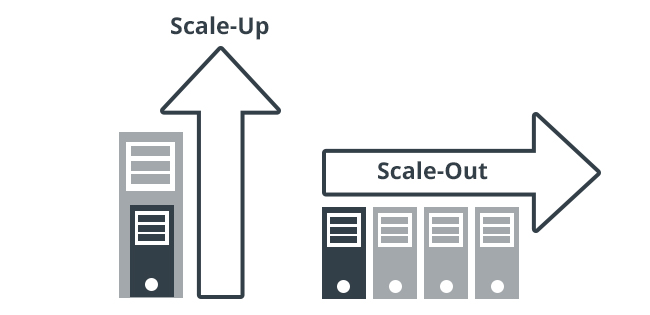
\includegraphics[width=0.7\textwidth]{resources/scales}
\caption[TEST]{TEST\protect\footnotemark}
\label{img:scales}
\end{figure}
\footnotetext{TEST: \url{https://magazin.kapilendo.de/den-supergau-verhindern-so-bereiten-sie-ihre-website-auf-einen-besucheransturm-vor/}, zugegriffen am 15. Januar 2017}
\section{Allgemein}

\begin{listingsboxJava}[label={lst:X}]{myJava}{Skript zur Initialisierung der Replikationsgruppe}
bla
\end{listingsboxJava} \clearpage
%\chapter{GUI-Schicht}
blabla
\section{Allgemein} \clearpage
%\chapter{Eine Cloud-Fotoalben-Verwaltung}
\section{Fachliche Spezifikation für die Endbenutzer}
Die folgende Spezifikation hat das Ziel, dem Endbenutzer die Grundprinzipien der geplanten webbasierten skalierbaren Anwendung für Fotoalben-Verwaltung zu präsentieren.
Die skalierbare Software für die webbasierte Fotoalben-Verwaltung ist geplant so zu implementieren, dass jeder sie als eigene Fotoalben-Verwaltung nutzen kann, unabhängig von wachsenden Ansprüchen an die Leistungsfähigkeit. 

\section{Anwendungsfälle}
Im Folgenden sind alle möglichen Szenarien dargestellt, die bei der Interaktion zwischen dem Besucher/Benutzer und des betrachteten Systems vorkommen können.

\subsection{Vorschau aller öffentlichen Fotoalben}
\begin{usecase}
\addtitle{Vorschau aller öffentlichen Fotoalben (=Preview of all public photo albums)}{}

\addfield{Kurzbeschreibung:}{Jeder Besucher kann alle vorhandenen öffentlichen Fotoalben sehen}
\addfield{Auslöser:}{Der Besucher verwendet den ihm bekannten Link für die Cloud-Fotoalben-Verwaltung}
\addfield{Eingabe:}{Den funktionierenden Link für die Cloud-Fotoalben-Verwaltung im Browser}
\addfield{Vorbedingung:}{Das System ist deployed}
\addfield{Ergebnis:}{Der Besucher landet auf die webbasierte Cloud-Fotoalben-Verwaltung und kann alle vorhandenen öffentlichen Fotoalben sehen}

\end{usecase}

\subsection{Fotoalbum ansehen}
\begin{usecase}
\addtitle{Ein Fotoalbum auswählen (= Show a photo album)}{}

\addfield{Kurzbeschreibung:}{Jeder Besucher kann den Inhalt jedes öffentlichen Fotoalbums ansehen}
\addfield{Auslöser:}{Der Besucher klickt auf das entsprechende Fotoalbum an, um seinen Inhalt ansehen zu können}
\addfield{Eingabe:}{\textbf{keine}}
\addfield{Vorbedingung:}{mind. ein Fotoalbum existiert}
\addfield{Ergebnis:}{Der Besucher kann den Inhalt des Fotoalbums sehen}

\end{usecase}

\subsection{Foto im Vollformat ansehen}
\begin{usecase}
\addtitle{Ein Foto im Vollformat ansehen (Show a photo in the full format)}{}

\addfield{Kurzbeschreibung:}{Jeder Besucher kann jedes Foto im Vollformat sehen}
\addfield{Auslöser:}{Der Besucher klickt auf das entsprechende Foto an, um es im Vollformat ansehen zu können}
\addfield{Eingabe:}{\textbf{keine}}
\addfield{Vorbedingung:}{mind. ein Foto existiert}
\addfield{Ergebnis:}{Der Besucher kann im Vollformat das Foto ansehen}

\end{usecase}

\subsection{Benutzerregistrierung}
\begin{usecase}
\addtitle{Registrierung (=Register)}{}

\addfield{Kurzbeschreibung:}{Ein Besucher registriert sich als neuer Benutzer }
\addfield{Auslöser:}{Der potentielle Benutzer klickt auf den Button \textbf{'Register'} und legt ein neues Benutzerkonto selbst an}
\addfield{Eingabe:}{Benutzername, Passwort und E-Mail sind für die Registrierung unbedingt einzugeben}
\addfield{Vorbedingung:}{Der potentielle Benutzer ist unter dem eingegebenen Benutzername im System noch nicht registriert}
\addfield{Ergebnis:}{Das Benutzerkonto für den neuen Benutzer wird im System angelegt. Der Benutzer wird nach der \textbf{'Registrierung'} an die Startseite weitergeleitet}

\end{usecase}

\subsection{Benutzeranmeldung}
\begin{usecase}
\addtitle{Anmeldung (=Login)}{}

\addfield{Kurzbeschreibung:}{Der registrierte Benutzer meldet sich im System an}
\addfield{Auslöser:}{Für die Anmeldung klickt der Benutzer auf den Button \textbf{'Please login'} und meldet sich mit seinem Benutzername und Passwort im System an}
\addfield{Eingabe:}{Benutzername und Passwort}
\addfield{Vorbedingung:}{Der Benutzer ist im System schon registriert}
\addfield{Ergebnis:}{Der Benutzer wird nach der erfolgreichen Anmeldung an eigene Startseite weitergeleitet}

\end{usecase}

\subsection{Fotoalbum anlegen}
\begin{usecase}
\addtitle{Fotoalbum anlegen (=Create a new photo album)}{}

\addfield{Kurzbeschreibung:}{Der angemeldete Benutzer legt sein neues Fotoalbum an}
\addfield{Auslöser:}{Für die Erzeugung eines neuen Fotoalbums klickt der Benutzer auf den Button \textbf{'Create a new photo album'}}
\addfield{Eingabe:}{Bezeichnung, Beschreibung und Abgrenzungsoption (= privat oder öffentlich) für sein zukünftiges Fotoalbum}
\addfield{Vorbedingung:}{Das Fotoalbum mit so einem Namen existiert bei dem angemeldeten Benutzer \textbf{nicht}}
\addfield{Ergebnis:}{Das Fotoalbum wird erzeugt und die Möglichkeit für das \textbf{'Select a photo for upload'} wird gleich freigeschaltet}

\end{usecase}

\subsection{Foto hochladen}
\begin{usecase}
\addtitle{Foto hochladen (=Upload a photo)}{}

\addfield{Kurzbeschreibung:}{Ein Benutzer lädt Fotos in ein existierendes Fotoalbum hoch}
\addfield{Auslöser:}{Für das Hochladen von Fotos in ein Fotoalbum klickt der Benutzer auf den Button \textbf{'Select a photo for upload'} und wählt ein Foto zum Hochladen aus}
\addfield{Eingabe:}{Gewünschtes Foto zum Hochladen auswählen}
\addfield{Vorbedingung:}{mind. ein Fotoalbum existiert}
\addfield{Ergebnis:}{Das ausgewählte Foto wird hochgeladen und die Möglichkeit für das \textbf{'Play a slideshow'} wird mit dem 1. hochgeladenen Foto gleich freigeschaltet}

\end{usecase}

\subsection{Foto löschen}
\begin{usecase}
\addtitle{Foto löschen (=Delete a photo)}{}

\addfield{Kurzbeschreibung:}{Nur ein registrierter Benutzer kann die eigenen Fotos aus den Fotoalben löschen}
\addfield{Auslöser:}{Für das Löschen von Fotos in einem Fotoalbum wählt der Benutzer bestimmte Fotos aus einem Fotoalbum aus und klickt auf den Button \textbf{'Delete n photos'}. \textbf{n} steht für die Anzahl von Fotos}
\addfield{Eingabe:}{\textbf{keine}}
\addfield{Vorbedingung:}{Die löschenden Fotos existieren}
\addfield{Ergebnis:}{Die markierten Fotos sind gelöscht und sind in dem Fotoalbum nicht mehr vorhanden}

\end{usecase}

\subsection{Fotoalbum löschen}
\begin{usecase}
\addtitle{Fotoalbum löschen (=Delete a photo album)}{}

\addfield{Kurzbeschreibung:}{Nur ein registrierter Benutzer kann die eigenen oder für ihn sichtbaren Fotoalben mit dem ganzen Inhalt löschen}
\addfield{Auslöser:}{Für das Löschen von Fotoalben klickt der Benutzer auf den Button \textbf{'Delete a photo album'}}
\addfield{Eingabe:}{\textbf{keine}}
\addfield{Vorbedingung:}{Das löschende Fotoalbum existiert}
\addfield{Ergebnis:}{Das Fotoalbum ist gelöscht und ist im System nicht mehr vorhanden}

\end{usecase}

\subsection{Foto-Diashow abspielen - \textbf{optional}}
\begin{usecase}
\addtitle{Foto-Diashow abspielen (=Play a slideshow)}{}

\addfield{Kurzbeschreibung:}{Ein Benutzer spielt Foto-Diashow ab}
\addfield{Auslöser:}{Für das Abspielen von Foto-Diashow klickt der Benutzer auf den Button \textbf{'Play a slideshow'}}
\addfield{Eingabe:}{\textbf{keine}}
\addfield{Vorbedingung:}{mind. ein Foto ist in einem Fotoalbum vorhanden}
\addfield{Ergebnis:}{Der Benutzer kann Foto-Diashow abspielen}

\end{usecase}

\subsection{Fotoalbum freigeben - \textbf{optional}}
\begin{usecase}
\addtitle{Fotoalbum freigeben (=Share a photo album)}{}

\addfield{Kurzbeschreibung:}{Ein Benutzer lädt seine Bekannte/Freunde/Verwandte zum einem bestimmten Fotoalbum per E-Mail ein, um dieses verwalten zu können}
\addfield{Auslöser:}{Für die Freigabe eines Fotoalbums klickt der Benutzer auf den Button \textbf{'Share a photo album'} und teilt per E-Mail über die Freigabe des Fotoalbums an die Gewünschten mit}
\addfield{Eingabe:}{Die E-Mail-Adressen von Bekannten/Freunden/Verwandten für die Freigabe}
\addfield{Vorbedingung:}{Der Eingeladene befindet sich nicht in der Liste der Freigegebenen}
\addfield{Ergebnis:}{Der Eingeladene kann ein freigegebenes Fotoalbum verwalten}

\end{usecase}

\subsection{Fotoalbum als Gast verwalten - \textbf{optional}}
\begin{usecase}
\addtitle{Fotoalbum als Gast verwalten (=Manage a photo album as guest)}{}

\addfield{Kurzbeschreibung:}{Ein Gast kann die für ihn freigegebenen Fotoalben verwalten}
\addfield{Auslöser:}{Eine Einladung per E-Mail, die eine Freigabe in Form eines Links verfügt}
\addfield{Eingabe:}{\textbf{keine}}
\addfield{Vorbedingung:}{Eine Freigabe per E-Mail}
\addfield{Ergebnis:}{Der eingeladene Gast kann das für ihn freigegebene Fotoalbum verwalten}

\end{usecase}

\subsection{Foto kommentieren - \textbf{optional}}
\begin{usecase}
\addtitle{Foto kommentieren (=Comment on a photo)}{}

\addfield{Kurzbeschreibung:}{Nur ein autorisierter Benutzer kann Fotos kommentieren}
\addfield{Auslöser:}{Für das Kommentieren von Fotos gibt der autorisierter Benutzer auf den Button \textbf{'Comment'} und gibt seinen Kommentar ein}
\addfield{Eingabe:}{Seine Meinung zu dem gewählten Foto}
\addfield{Vorbedingung:}{mind. ein Foto ist in einem Fotoalbum vorhanden und der Benutzer darf nicht unauthentifiziert sein}
\addfield{Ergebnis:}{Das Foto verfügt über einen \textbf{neuen} Kommentar}

\end{usecase}

%\subsection{}
%\begin{usecase}
%\addtitle{}{}
%
%\addfield{Kurzbeschreibung:}{}
%\addfield{Auslöser:}{}
%\addfield{Eingabe:}{}
%\addfield{Vorbedingung:}{}
%\addfield{Ergebnis:}{}
%
%\end{usecase}

%\section{Technische Spezifikation für die Entwickler}

%Eine technische Spezifikation dient dem Entwickler zur Orientierung, wie die geplante Software strukturiert ist und wie die in der Abbildung XXX dargestellten Module zusammenspielen, welche Frameworks, Programmiersprachen für Frontend und Backend genutzt werden.

 \clearpage

\pagenumbering{Alph}
\printbibliography[heading=bibintoc, keyword={book}, title={Literaturverzeichnis}]
\printbibliography[heading=bibintoc, keyword={online}, title={Verzeichnis der Webadressen}]

\listoffigures \clearpage
\listoftables \clearpage
\printbibliography[heading=bibintoc, keyword={image}, title={Bildquellen}]\clearpage
\tcblistof[\chapter*]{mybox}{Quelltextverzeichnis}

\end{document}